% Generated by Sphinx.
\def\sphinxdocclass{report}
\documentclass[letterpaper,10pt,english]{sphinxmanual}
\usepackage[utf8]{inputenc}
\DeclareUnicodeCharacter{00A0}{\nobreakspace}
\usepackage{cmap}
\usepackage[T1]{fontenc}
\usepackage{babel}
\usepackage{times}
\usepackage[Bjarne]{fncychap}
\usepackage{longtable}
\usepackage{sphinx}
\usepackage{multirow}


\title{Effective Django}
\date{10 March 2015}
\release{}
\author{Nathan Yergler}
\newcommand{\sphinxlogo}{}
\renewcommand{\releasename}{Build 2015.03.10}
\makeindex

\makeatletter
\def\PYG@reset{\let\PYG@it=\relax \let\PYG@bf=\relax%
    \let\PYG@ul=\relax \let\PYG@tc=\relax%
    \let\PYG@bc=\relax \let\PYG@ff=\relax}
\def\PYG@tok#1{\csname PYG@tok@#1\endcsname}
\def\PYG@toks#1+{\ifx\relax#1\empty\else%
    \PYG@tok{#1}\expandafter\PYG@toks\fi}
\def\PYG@do#1{\PYG@bc{\PYG@tc{\PYG@ul{%
    \PYG@it{\PYG@bf{\PYG@ff{#1}}}}}}}
\def\PYG#1#2{\PYG@reset\PYG@toks#1+\relax+\PYG@do{#2}}

\expandafter\def\csname PYG@tok@gd\endcsname{\def\PYG@tc##1{\textcolor[rgb]{0.63,0.00,0.00}{##1}}}
\expandafter\def\csname PYG@tok@gu\endcsname{\let\PYG@bf=\textbf\def\PYG@tc##1{\textcolor[rgb]{0.50,0.00,0.50}{##1}}}
\expandafter\def\csname PYG@tok@gt\endcsname{\def\PYG@tc##1{\textcolor[rgb]{0.00,0.27,0.87}{##1}}}
\expandafter\def\csname PYG@tok@gs\endcsname{\let\PYG@bf=\textbf}
\expandafter\def\csname PYG@tok@gr\endcsname{\def\PYG@tc##1{\textcolor[rgb]{1.00,0.00,0.00}{##1}}}
\expandafter\def\csname PYG@tok@cm\endcsname{\let\PYG@it=\textit\def\PYG@tc##1{\textcolor[rgb]{0.25,0.50,0.56}{##1}}}
\expandafter\def\csname PYG@tok@vg\endcsname{\def\PYG@tc##1{\textcolor[rgb]{0.73,0.38,0.84}{##1}}}
\expandafter\def\csname PYG@tok@m\endcsname{\def\PYG@tc##1{\textcolor[rgb]{0.13,0.50,0.31}{##1}}}
\expandafter\def\csname PYG@tok@mh\endcsname{\def\PYG@tc##1{\textcolor[rgb]{0.13,0.50,0.31}{##1}}}
\expandafter\def\csname PYG@tok@cs\endcsname{\def\PYG@tc##1{\textcolor[rgb]{0.25,0.50,0.56}{##1}}\def\PYG@bc##1{\setlength{\fboxsep}{0pt}\colorbox[rgb]{1.00,0.94,0.94}{\strut ##1}}}
\expandafter\def\csname PYG@tok@ge\endcsname{\let\PYG@it=\textit}
\expandafter\def\csname PYG@tok@vc\endcsname{\def\PYG@tc##1{\textcolor[rgb]{0.73,0.38,0.84}{##1}}}
\expandafter\def\csname PYG@tok@il\endcsname{\def\PYG@tc##1{\textcolor[rgb]{0.13,0.50,0.31}{##1}}}
\expandafter\def\csname PYG@tok@go\endcsname{\def\PYG@tc##1{\textcolor[rgb]{0.20,0.20,0.20}{##1}}}
\expandafter\def\csname PYG@tok@cp\endcsname{\def\PYG@tc##1{\textcolor[rgb]{0.00,0.44,0.13}{##1}}}
\expandafter\def\csname PYG@tok@gi\endcsname{\def\PYG@tc##1{\textcolor[rgb]{0.00,0.63,0.00}{##1}}}
\expandafter\def\csname PYG@tok@gh\endcsname{\let\PYG@bf=\textbf\def\PYG@tc##1{\textcolor[rgb]{0.00,0.00,0.50}{##1}}}
\expandafter\def\csname PYG@tok@ni\endcsname{\let\PYG@bf=\textbf\def\PYG@tc##1{\textcolor[rgb]{0.84,0.33,0.22}{##1}}}
\expandafter\def\csname PYG@tok@nl\endcsname{\let\PYG@bf=\textbf\def\PYG@tc##1{\textcolor[rgb]{0.00,0.13,0.44}{##1}}}
\expandafter\def\csname PYG@tok@nn\endcsname{\let\PYG@bf=\textbf\def\PYG@tc##1{\textcolor[rgb]{0.05,0.52,0.71}{##1}}}
\expandafter\def\csname PYG@tok@no\endcsname{\def\PYG@tc##1{\textcolor[rgb]{0.38,0.68,0.84}{##1}}}
\expandafter\def\csname PYG@tok@na\endcsname{\def\PYG@tc##1{\textcolor[rgb]{0.25,0.44,0.63}{##1}}}
\expandafter\def\csname PYG@tok@nb\endcsname{\def\PYG@tc##1{\textcolor[rgb]{0.00,0.44,0.13}{##1}}}
\expandafter\def\csname PYG@tok@nc\endcsname{\let\PYG@bf=\textbf\def\PYG@tc##1{\textcolor[rgb]{0.05,0.52,0.71}{##1}}}
\expandafter\def\csname PYG@tok@nd\endcsname{\let\PYG@bf=\textbf\def\PYG@tc##1{\textcolor[rgb]{0.33,0.33,0.33}{##1}}}
\expandafter\def\csname PYG@tok@ne\endcsname{\def\PYG@tc##1{\textcolor[rgb]{0.00,0.44,0.13}{##1}}}
\expandafter\def\csname PYG@tok@nf\endcsname{\def\PYG@tc##1{\textcolor[rgb]{0.02,0.16,0.49}{##1}}}
\expandafter\def\csname PYG@tok@si\endcsname{\let\PYG@it=\textit\def\PYG@tc##1{\textcolor[rgb]{0.44,0.63,0.82}{##1}}}
\expandafter\def\csname PYG@tok@s2\endcsname{\def\PYG@tc##1{\textcolor[rgb]{0.25,0.44,0.63}{##1}}}
\expandafter\def\csname PYG@tok@vi\endcsname{\def\PYG@tc##1{\textcolor[rgb]{0.73,0.38,0.84}{##1}}}
\expandafter\def\csname PYG@tok@nt\endcsname{\let\PYG@bf=\textbf\def\PYG@tc##1{\textcolor[rgb]{0.02,0.16,0.45}{##1}}}
\expandafter\def\csname PYG@tok@nv\endcsname{\def\PYG@tc##1{\textcolor[rgb]{0.73,0.38,0.84}{##1}}}
\expandafter\def\csname PYG@tok@s1\endcsname{\def\PYG@tc##1{\textcolor[rgb]{0.25,0.44,0.63}{##1}}}
\expandafter\def\csname PYG@tok@gp\endcsname{\let\PYG@bf=\textbf\def\PYG@tc##1{\textcolor[rgb]{0.78,0.36,0.04}{##1}}}
\expandafter\def\csname PYG@tok@sh\endcsname{\def\PYG@tc##1{\textcolor[rgb]{0.25,0.44,0.63}{##1}}}
\expandafter\def\csname PYG@tok@ow\endcsname{\let\PYG@bf=\textbf\def\PYG@tc##1{\textcolor[rgb]{0.00,0.44,0.13}{##1}}}
\expandafter\def\csname PYG@tok@sx\endcsname{\def\PYG@tc##1{\textcolor[rgb]{0.78,0.36,0.04}{##1}}}
\expandafter\def\csname PYG@tok@bp\endcsname{\def\PYG@tc##1{\textcolor[rgb]{0.00,0.44,0.13}{##1}}}
\expandafter\def\csname PYG@tok@c1\endcsname{\let\PYG@it=\textit\def\PYG@tc##1{\textcolor[rgb]{0.25,0.50,0.56}{##1}}}
\expandafter\def\csname PYG@tok@kc\endcsname{\let\PYG@bf=\textbf\def\PYG@tc##1{\textcolor[rgb]{0.00,0.44,0.13}{##1}}}
\expandafter\def\csname PYG@tok@c\endcsname{\let\PYG@it=\textit\def\PYG@tc##1{\textcolor[rgb]{0.25,0.50,0.56}{##1}}}
\expandafter\def\csname PYG@tok@mf\endcsname{\def\PYG@tc##1{\textcolor[rgb]{0.13,0.50,0.31}{##1}}}
\expandafter\def\csname PYG@tok@err\endcsname{\def\PYG@bc##1{\setlength{\fboxsep}{0pt}\fcolorbox[rgb]{1.00,0.00,0.00}{1,1,1}{\strut ##1}}}
\expandafter\def\csname PYG@tok@mb\endcsname{\def\PYG@tc##1{\textcolor[rgb]{0.13,0.50,0.31}{##1}}}
\expandafter\def\csname PYG@tok@ss\endcsname{\def\PYG@tc##1{\textcolor[rgb]{0.32,0.47,0.09}{##1}}}
\expandafter\def\csname PYG@tok@sr\endcsname{\def\PYG@tc##1{\textcolor[rgb]{0.14,0.33,0.53}{##1}}}
\expandafter\def\csname PYG@tok@mo\endcsname{\def\PYG@tc##1{\textcolor[rgb]{0.13,0.50,0.31}{##1}}}
\expandafter\def\csname PYG@tok@kd\endcsname{\let\PYG@bf=\textbf\def\PYG@tc##1{\textcolor[rgb]{0.00,0.44,0.13}{##1}}}
\expandafter\def\csname PYG@tok@mi\endcsname{\def\PYG@tc##1{\textcolor[rgb]{0.13,0.50,0.31}{##1}}}
\expandafter\def\csname PYG@tok@kn\endcsname{\let\PYG@bf=\textbf\def\PYG@tc##1{\textcolor[rgb]{0.00,0.44,0.13}{##1}}}
\expandafter\def\csname PYG@tok@o\endcsname{\def\PYG@tc##1{\textcolor[rgb]{0.40,0.40,0.40}{##1}}}
\expandafter\def\csname PYG@tok@kr\endcsname{\let\PYG@bf=\textbf\def\PYG@tc##1{\textcolor[rgb]{0.00,0.44,0.13}{##1}}}
\expandafter\def\csname PYG@tok@s\endcsname{\def\PYG@tc##1{\textcolor[rgb]{0.25,0.44,0.63}{##1}}}
\expandafter\def\csname PYG@tok@kp\endcsname{\def\PYG@tc##1{\textcolor[rgb]{0.00,0.44,0.13}{##1}}}
\expandafter\def\csname PYG@tok@w\endcsname{\def\PYG@tc##1{\textcolor[rgb]{0.73,0.73,0.73}{##1}}}
\expandafter\def\csname PYG@tok@kt\endcsname{\def\PYG@tc##1{\textcolor[rgb]{0.56,0.13,0.00}{##1}}}
\expandafter\def\csname PYG@tok@sc\endcsname{\def\PYG@tc##1{\textcolor[rgb]{0.25,0.44,0.63}{##1}}}
\expandafter\def\csname PYG@tok@sb\endcsname{\def\PYG@tc##1{\textcolor[rgb]{0.25,0.44,0.63}{##1}}}
\expandafter\def\csname PYG@tok@k\endcsname{\let\PYG@bf=\textbf\def\PYG@tc##1{\textcolor[rgb]{0.00,0.44,0.13}{##1}}}
\expandafter\def\csname PYG@tok@se\endcsname{\let\PYG@bf=\textbf\def\PYG@tc##1{\textcolor[rgb]{0.25,0.44,0.63}{##1}}}
\expandafter\def\csname PYG@tok@sd\endcsname{\let\PYG@it=\textit\def\PYG@tc##1{\textcolor[rgb]{0.25,0.44,0.63}{##1}}}

\def\PYGZbs{\char`\\}
\def\PYGZus{\char`\_}
\def\PYGZob{\char`\{}
\def\PYGZcb{\char`\}}
\def\PYGZca{\char`\^}
\def\PYGZam{\char`\&}
\def\PYGZlt{\char`\<}
\def\PYGZgt{\char`\>}
\def\PYGZsh{\char`\#}
\def\PYGZpc{\char`\%}
\def\PYGZdl{\char`\$}
\def\PYGZhy{\char`\-}
\def\PYGZsq{\char`\'}
\def\PYGZdq{\char`\"}
\def\PYGZti{\char`\~}
% for compatibility with earlier versions
\def\PYGZat{@}
\def\PYGZlb{[}
\def\PYGZrb{]}
\makeatother

\renewcommand\PYGZsq{\textquotesingle}

\begin{document}

\maketitle
\tableofcontents
\phantomsection\label{tutorial/index::doc}


\begin{notice}{note}{Note:}
\href{https://www.youtube.com/watch?v=NfsJDPm0X54}{Video of this tutorial} (https://www.youtube.com/watch?v=NfsJDPm0X54) from PyCon is available on YouTube.
\end{notice}

Django is a popular, powerful web framework for Python. It has lots of
``batteries'' included, and makes it easy to get up and going. But all
of the power means you can write low quality code that still seems to
work. So what does \emph{Effective Django} mean? It means using Django in a
way that emphasizes writing code that's cohesive, testable, and
scalable. What do each of those words mean?

Well, ``cohesive'' code is code that is focused on doing one thing, and
one thing alone. It means that when you write a function or a method,
that it does one thing and does it well.

This is directly related to writing testable code: code that's doing
too much is often difficult to write tests for. When I find myself
thinking, ``Well, this piece of code is just too complex to write a
test for, it's not really worth all the effort,'' that's a signal that
I need to step back and focus on simplifying it. Testable code is code
that makes it straight-forward to write tests for, and that's easy to
diagnose problems with.

Finally, we want to write scalable code. That doesn't just mean it
scales in terms of performance, but that it also scales in terms of
your team and your team's understanding. Applications that are well
tested are easier for others to understand (and easier for them to
modify), which means you're more able to improve your application by
adding engineers.

My goal is to convince you of the importance of these principles, and
provide examples of how to follow them to build more robust Django
applications. I'm going to walk through building a contact management
application iteratively, talking about the choices and testing
strategy as I go.

The sample code for this tutorial is available in the
\href{https://github.com/nyergler/effective-django-tutorial/}{effective-django-tutorial} (https://github.com/nyergler/effective-django-tutorial/) git repository.

Slides for the tutorial are available at \href{http://effectivedjango.com/slides/tutorial}{http://effectivedjango.com/slides/tutorial}
\DUspan{admonition-effective-django}{}\DUspan{admonition-goals}{}\DUspan{admonition-effective}{}

\chapter{Getting Started}
\label{tutorial/getting-started:getting-started}\label{tutorial/getting-started::doc}\label{tutorial/getting-started:effective-django-tutorial}

\section{Your Development Environment}
\label{tutorial/getting-started:your-development-environment}\DUspan{admonition-the-environment}{}
When thinking about your development environment, there are three
important things to keep in mind: isolation, determinism, and
similarity. They're each important, and they work in concert with one
another.

\textbf{Isolation} means that you're not inadvertently leveraging tools
or packages installed outside the environment. This is particularly
important when it comes to something like Python packages with C
extensions: if you're using something installed at the system level
and don't know it, you can find that when you go to deploy or share
your code that it doesn't operate the way you expect. A tool like
\href{http://www.virtualenv.org/}{virtualenv} (http://www.virtualenv.org/) can help create that sort of environment.

Your environment is \textbf{deterministic} if you're confident about
what versions of your dependencies you're relying on, and can
reproduce that environment reliably.

Finally, \textbf{similarity} to your production or deployment
environment means you're running on the same OS, preferably the
same release, and that you're using the same tools to configure
your development environment that you use to configure your
deployment environment. This is by no means a requirement, but as
you build bigger, more complex software, it's helpful to be
confident that any problem you see in production is reproducable in
your development environment, and limit the scope of investigation
to code you wrote.


\subsection{Isolation}
\label{tutorial/getting-started:virtualenv}\label{tutorial/getting-started:isolation}\begin{itemize}
\item {} 
We want to avoid using unknown dependencies, or unknown versions

\item {} 
\href{http://www.virtualenv.org/}{virtualenv} (http://www.virtualenv.org/) provides an easy way to work on a project without your
system's \code{site-packages}

\end{itemize}


\subsection{Determinism}
\label{tutorial/getting-started:determinism}\begin{itemize}
\item {} 
Determinism is all about dependency management

\item {} 
Choose a tool, use it in development and production
\begin{itemize}
\item {} 
pip, specifically a \href{http://www.pip-installer.org/en/latest/requirements.html}{requirements files} (http://www.pip-installer.org/en/latest/requirements.html)

\item {} 
\href{http://www.buildout.org/}{buildout} (http://www.buildout.org/)

\item {} 
\href{http://pythonhosted.org/distribute/setuptools.html\#declaring-dependencies}{install\_requires} (http://pythonhosted.org/distribute/setuptools.html\#declaring-dependencies) in setup.py

\end{itemize}

\item {} 
Identify specific versions of dependencies

\end{itemize}

You can specify versions either by the version for a package on
PyPI, or a specific revision (SHA in git, revision number in
Subversion, etc). This ensures that you're getting the exact
version you're testing with.


\subsection{Similarity}
\label{tutorial/getting-started:install-requires}\label{tutorial/getting-started:similarity}\begin{itemize}
\item {} 
Working in an environment similar to where you deploy eliminates
variables when trying to diagnose an issue

\item {} 
If you're building something that requires additional services, this
becomes even more important.

\item {} 
\href{http://vagrantup.com/}{Vagrant} (http://vagrantup.com/) is a tool for managing virtual machines, lets you easily
create an environment separate from your day to day work.

\end{itemize}


\section{Setting Up Your Environment}
\label{tutorial/getting-started:setting-up-your-environment}\label{tutorial/getting-started:vagrant}

\subsection{Create a Clean Workspace}
\label{tutorial/getting-started:create-a-clean-workspace}
\begin{Verbatim}[commandchars=\\\{\}]
\PYGZdl{} mkdir tutorial
\PYGZdl{} virtualenv ./tutorial/
New python executable in ./tutorial/bin/python
Installing setuptools............done.
Installing pip...............done.
\PYGZdl{} source ./tutorial/bin/activate
(tutorial)\PYGZdl{}
\end{Verbatim}


\subsection{Start a Requirements File}
\label{tutorial/getting-started:example-repository}\label{tutorial/getting-started:start-a-requirements-file}
Create a \code{requirements.txt} in the \code{tutorial} directory with a
single requirement in it.

\begin{Verbatim}[commandchars=\\\{\}]
Django==1.5.1
\end{Verbatim}


\subsection{Installing Requirements}
\label{tutorial/getting-started:installing-requirements}
And then we can use \href{http://www.pip-installer.org/}{pip} (http://www.pip-installer.org/) to install the dependencies.

\begin{Verbatim}[commandchars=\\\{\}]
(tutorial)\PYGZdl{} pip install \PYGZhy{}U \PYGZhy{}r requirements.txt

Downloading/unpacking Django==1.5.1
  Downloading Django\PYGZhy{}1.5.1.tar.gz (8.0MB): 8.0MB downloaded
  Running setup.py egg\PYGZus{}info for package Django

    warning: no previously\PYGZhy{}included files matching \PYGZsq{}\PYGZus{}\PYGZus{}pycache\PYGZus{}\PYGZus{}\PYGZsq{} found under directory \PYGZsq{}*\PYGZsq{}
    warning: no previously\PYGZhy{}included files matching \PYGZsq{}*.py[co]\PYGZsq{} found under directory \PYGZsq{}*\PYGZsq{}
Installing collected packages: Django
  Running setup.py install for Django
    changing mode of build/scripts\PYGZhy{}2.7/django\PYGZhy{}admin.py from 644 to 755

    warning: no previously\PYGZhy{}included files matching \PYGZsq{}\PYGZus{}\PYGZus{}pycache\PYGZus{}\PYGZus{}\PYGZsq{} found under directory \PYGZsq{}*\PYGZsq{}
    warning: no previously\PYGZhy{}included files matching \PYGZsq{}*.py[co]\PYGZsq{} found under directory \PYGZsq{}*\PYGZsq{}
    changing mode of /home/nathan/p/edt/bin/django\PYGZhy{}admin.py to 755
Successfully installed Django
Cleaning up...
\end{Verbatim}


\section{Beginning a Django Project}
\label{tutorial/getting-started:pip}\label{tutorial/getting-started:beginning-a-django-project}
When a building is under construction, scaffolding is often used to
support the structure before it's complete. The scaffolding can be
temporary, or it can serve as part of the foundation for the
building, but regardless it provides some support when you're just
starting out.

Django, like many web frameworks, provides scaffolding for your
development efforts. It does this by making decisions and providing
a starting point for your code that lets you focus on the problem
you're trying to solve, and not how to parse an HTTP request.
Django provides HTTP, as well as file system scaffolding.

The HTTP scaffolding handles things like parsing an HTTP request
into a Python object and providing tools to easily create a
response. The file system scaffolding is a little different: it's a
set of conventions for organizing your code. These conventions make
it easier to add engineers to a project, since they
(hypothetically) have some idea how the code is organized. In
Django parlance, a \textbf{project} is the final product, and it
assembles one or more \textbf{applications} together. Django 1.4 made a
change to the way the \href{https://docs.djangoproject.com/en/1.5/releases/1.4/\#updated-default-project-layout-and-manage-py}{projects and applications are laid out on
disk} (https://docs.djangoproject.com/en/1.5/releases/1.4/\#updated-default-project-layout-and-manage-py), which makes it easier to decouple and reuse applications
between projects.
\DUspan{admonition-scaffolding}{}

\subsection{Creating the Project}
\label{tutorial/getting-started:creating-the-project}
Django installs a \code{django-admin.py} script for handling scaffolding
tasks. We'll use \code{startproject} to create the project files. We
specify the project name and the directory to start in; we're already
in our isolated environment so we can just say \code{.}

\begin{Verbatim}[commandchars=\\\{\}]
(tutorial)\PYGZdl{} django\PYGZhy{}admin.py startproject addressbook .
\end{Verbatim}

\begin{Verbatim}[commandchars=\\\{\}]
manage.py
./addressbook
    \PYGZus{}\PYGZus{}init\PYGZus{}\PYGZus{}.py
    settings.py
    urls.py
    wsgi.py
\end{Verbatim}


\subsection{Project Scaffolding}
\label{tutorial/getting-started:project-scaffolding}\begin{itemize}
\item {} 
\code{manage.py} is a pointer back to \code{django-admin.py} with an
environment variable set, pointing to your project as the one to
read settings from and operate on when needed.

\item {} 
\code{settings.py} is where you'll configure your project. It has a
few sensible defaults, but no database chosen when you start.

\item {} 
\code{urls.py} contains the URL to view mappings: we'll talk more about
that shortly.

\item {} 
\code{wsgi.py} is a \href{https://en.wikipedia.org/wiki/Web\_Server\_Gateway\_Interface}{WSGI} (https://en.wikipedia.org/wiki/Web\_Server\_Gateway\_Interface) wrapper for your application. This is used
by Django's development servers, and possibly other containers
like mod\_wsgi, uwsgi, etc. in production.

\end{itemize}


\subsection{Creating the ``App''}
\label{tutorial/getting-started:creating-the-app}\label{tutorial/getting-started:wsgi}
\begin{Verbatim}[commandchars=\\\{\}]
(tutorial)\PYGZdl{} python ./manage.py startapp contacts
\end{Verbatim}

\begin{Verbatim}[commandchars=\\\{\}]
./addressbook
./contacts
    \PYGZus{}\PYGZus{}init\PYGZus{}\PYGZus{}.py
    models.py
    tests.py
    views.py
\end{Verbatim}
\begin{itemize}
\item {} 
Beginning in Django 1.4, \emph{apps} are placed alongside \emph{project}
packages. This is a great improvement when it comes to
deployment.

\item {} 
\code{models.py} will contain the Django ORM models for your app.

\item {} 
\code{views.py} will contain the View code

\item {} 
\code{tests.py} will contain the unit and integration tests you
write.

\end{itemize}
\DUspan{admonition-review}{}

\chapter{Using Models}
\label{tutorial/models::doc}\label{tutorial/models:using-models}\DUspan{admonition-django-models}{}

\section{Configuring the Database}
\label{tutorial/models:configuring-the-database}\DUspan{admonition-configuring-databases}{}
Django includes support out of the box for MySQL, PostgreSQL, SQLite3,
and Oracle. \href{http://docs.python.org/2/library/sqlite3.html}{SQLite3} (http://docs.python.org/2/library/sqlite3.html) is included with Python starting with version
2.5, so we'll use it for our project for simplicity. If you were going
to use MySQL, for example, you'd need to add \href{https://pypi.python.org/pypi/MySQL-python}{mysql-python} (https://pypi.python.org/pypi/MySQL-python) to your
\code{requirements.txt} file.

To enable SQLite as the database, edit the \code{DATABASES} definition in
\code{addressbook/settings.py}. The \code{settings.py} file contains the
Django configuration for our project. There are some settings that you
must specify -- like the \code{DATABASES} configuration -- and others
that are optional. Django fills in some defaults when it generates the
project scaffolding, and the documentation contains a \href{https://docs.djangoproject.com/en/1.5/ref/settings/}{full list of
settings} (https://docs.djangoproject.com/en/1.5/ref/settings/). You can also add your own settings here, if needed.

For SQLite we need to set the engine and then give it a name. The
SQLite backend uses the \code{NAME} as the filename for the database.

\begin{Verbatim}[commandchars=\\\{\}]
\PYG{n}{DATABASES} \PYG{o}{=} \PYG{p}{\PYGZob{}}
    \PYG{l+s}{\PYGZsq{}}\PYG{l+s}{default}\PYG{l+s}{\PYGZsq{}}\PYG{p}{:} \PYG{p}{\PYGZob{}}
        \PYG{l+s}{\PYGZsq{}}\PYG{l+s}{ENGINE}\PYG{l+s}{\PYGZsq{}}\PYG{p}{:} \PYG{l+s}{\PYGZsq{}}\PYG{l+s}{django.db.backends.sqlite3}\PYG{l+s}{\PYGZsq{}}\PYG{p}{,}  \PYG{c}{\PYGZsh{} \PYGZsq{}postgresql\PYGZus{}psycopg2\PYGZsq{}, \PYGZsq{}mysql\PYGZsq{}, \PYGZsq{}sqlite3\PYGZsq{} or \PYGZsq{}oracle\PYGZsq{}.}
        \PYG{l+s}{\PYGZsq{}}\PYG{l+s}{NAME}\PYG{l+s}{\PYGZsq{}}\PYG{p}{:} \PYG{l+s}{\PYGZsq{}}\PYG{l+s}{address.db}\PYG{l+s}{\PYGZsq{}}\PYG{p}{,}
        \PYG{l+s}{\PYGZsq{}}\PYG{l+s}{USER}\PYG{l+s}{\PYGZsq{}}\PYG{p}{:} \PYG{l+s}{\PYGZsq{}}\PYG{l+s}{\PYGZsq{}}\PYG{p}{,}                      \PYG{c}{\PYGZsh{} Not used with sqlite3.}
        \PYG{l+s}{\PYGZsq{}}\PYG{l+s}{PASSWORD}\PYG{l+s}{\PYGZsq{}}\PYG{p}{:} \PYG{l+s}{\PYGZsq{}}\PYG{l+s}{\PYGZsq{}}\PYG{p}{,}                  \PYG{c}{\PYGZsh{} Not used with sqlite3.}
        \PYG{l+s}{\PYGZsq{}}\PYG{l+s}{HOST}\PYG{l+s}{\PYGZsq{}}\PYG{p}{:} \PYG{l+s}{\PYGZsq{}}\PYG{l+s}{\PYGZsq{}}\PYG{p}{,}                      \PYG{c}{\PYGZsh{} Set to empty string for localhost. Not used with sqlite3.}
        \PYG{l+s}{\PYGZsq{}}\PYG{l+s}{PORT}\PYG{l+s}{\PYGZsq{}}\PYG{p}{:} \PYG{l+s}{\PYGZsq{}}\PYG{l+s}{\PYGZsq{}}\PYG{p}{,}                      \PYG{c}{\PYGZsh{} Set to empty string for default. Not used with sqlite3.}
    \PYG{p}{\PYGZcb{}}
\PYG{p}{\PYGZcb{}}
\end{Verbatim}

Note that the database engine is specified as a string, and not a
direct reference to the Python object. This is because the settings
file needs to be easily importable, without triggering any side
effects. You should avoid adding imports to the settings file.

You rarely need to import the settings file directly; Django imports
it for you, and makes it available as \code{django.conf.settings}. You
typically import your settings from \code{django.conf}:

\begin{Verbatim}[commandchars=\\\{\}]
\PYG{k+kn}{from} \PYG{n+nn}{django.conf} \PYG{k+kn}{import} \PYG{n}{settings}
\end{Verbatim}


\section{Creating a Model}
\label{tutorial/models:creating-a-model}\DUspan{admonition-defining-models}{}
Django models map (roughly) to a database table, and provide a place
to encapsulate business logic. All models subclass the base \href{https://docs.djangoproject.com/en/1.5/ref/models/instances/\#django.db.models.Model}{Model} (https://docs.djangoproject.com/en/1.5/ref/models/instances/\#django.db.models.Model)
class, and contain field definitions. Let's start by creating a simple
Contact model for our application in \code{contacts/models.py}.

\begin{Verbatim}[commandchars=\\\{\}]
\PYG{k+kn}{from} \PYG{n+nn}{django.db} \PYG{k+kn}{import} \PYG{n}{models}


\PYG{k}{class} \PYG{n+nc}{Contact}\PYG{p}{(}\PYG{n}{models}\PYG{o}{.}\PYG{n}{Model}\PYG{p}{)}\PYG{p}{:}

    \PYG{n}{first\PYGZus{}name} \PYG{o}{=} \PYG{n}{models}\PYG{o}{.}\PYG{n}{CharField}\PYG{p}{(}
        \PYG{n}{max\PYGZus{}length}\PYG{o}{=}\PYG{l+m+mi}{255}\PYG{p}{,}
    \PYG{p}{)}
    \PYG{n}{last\PYGZus{}name} \PYG{o}{=} \PYG{n}{models}\PYG{o}{.}\PYG{n}{CharField}\PYG{p}{(}
        \PYG{n}{max\PYGZus{}length}\PYG{o}{=}\PYG{l+m+mi}{255}\PYG{p}{,}

    \PYG{p}{)}

    \PYG{n}{email} \PYG{o}{=} \PYG{n}{models}\PYG{o}{.}\PYG{n}{EmailField}\PYG{p}{(}\PYG{p}{)}

    \PYG{k}{def} \PYG{n+nf}{\PYGZus{}\PYGZus{}str\PYGZus{}\PYGZus{}}\PYG{p}{(}\PYG{n+nb+bp}{self}\PYG{p}{)}\PYG{p}{:}

        \PYG{k}{return} \PYG{l+s}{\PYGZsq{}}\PYG{l+s}{ }\PYG{l+s}{\PYGZsq{}}\PYG{o}{.}\PYG{n}{join}\PYG{p}{(}\PYG{p}{[}
            \PYG{n+nb+bp}{self}\PYG{o}{.}\PYG{n}{first\PYGZus{}name}\PYG{p}{,}
            \PYG{n+nb+bp}{self}\PYG{o}{.}\PYG{n}{last\PYGZus{}name}\PYG{p}{,}
        \PYG{p}{]}\PYG{p}{)}
\end{Verbatim}

Django provides a set of \href{https://docs.djangoproject.com/en/1.5/ref/models/fields/}{fields} (https://docs.djangoproject.com/en/1.5/ref/models/fields/) that map to data types and different
validation rules. For example, the \code{EmailField} here maps to the
same column type as the \code{CharField}, but adds validation for the
data.

Once you've created a model, you need to update your database with the
new tables. Django's \code{syncdb} command looks for models that are
installed and creates tables for them if needed.

\begin{Verbatim}[commandchars=\\\{\}]
(tutorial)\PYGZdl{} python ./manage.py syncdb

Creating tables ...
Creating table auth\PYGZus{}permission
Creating table auth\PYGZus{}group\PYGZus{}permissions
Creating table auth\PYGZus{}group
Creating table auth\PYGZus{}user\PYGZus{}user\PYGZus{}permissions
Creating table auth\PYGZus{}user\PYGZus{}groups
Creating table auth\PYGZus{}user
Creating table django\PYGZus{}content\PYGZus{}type
Creating table django\PYGZus{}session
Creating table django\PYGZus{}site

...
\end{Verbatim}

Our contact table isn't anywhere to be seen. The reason is that we
need to tell the Project to use the Application.

The \code{INSTALLED\_APPS} setting lists the applications that the project
uses. These are listed as strings that map to Python packages. Django
will import each and looks for a \code{models} module there. Add our
Contacts app to the project's \code{INSTALLED\_APPS} setting:

\begin{Verbatim}[commandchars=\\\{\}]
\PYG{n}{INSTALLED\PYGZus{}APPS} \PYG{o}{=} \PYG{p}{(}
    \PYG{l+s}{\PYGZsq{}}\PYG{l+s}{django.contrib.auth}\PYG{l+s}{\PYGZsq{}}\PYG{p}{,}
    \PYG{l+s}{\PYGZsq{}}\PYG{l+s}{django.contrib.contenttypes}\PYG{l+s}{\PYGZsq{}}\PYG{p}{,}
    \PYG{l+s}{\PYGZsq{}}\PYG{l+s}{django.contrib.sessions}\PYG{l+s}{\PYGZsq{}}\PYG{p}{,}
    \PYG{l+s}{\PYGZsq{}}\PYG{l+s}{django.contrib.sites}\PYG{l+s}{\PYGZsq{}}\PYG{p}{,}
    \PYG{l+s}{\PYGZsq{}}\PYG{l+s}{django.contrib.messages}\PYG{l+s}{\PYGZsq{}}\PYG{p}{,}
    \PYG{l+s}{\PYGZsq{}}\PYG{l+s}{django.contrib.staticfiles}\PYG{l+s}{\PYGZsq{}}\PYG{p}{,}
    \PYG{c}{\PYGZsh{} Uncomment the next line to enable the admin:}
    \PYG{c}{\PYGZsh{} \PYGZsq{}django.contrib.admin\PYGZsq{},}
    \PYG{c}{\PYGZsh{} Uncomment the next line to enable admin documentation:}
    \PYG{c}{\PYGZsh{} \PYGZsq{}django.contrib.admindocs\PYGZsq{},}
    \PYG{l+s}{\PYGZsq{}}\PYG{l+s}{contacts}\PYG{l+s}{\PYGZsq{}}\PYG{p}{,}
\PYG{p}{)}
\end{Verbatim}

Then run \code{syncdb} again:

\begin{Verbatim}[commandchars=\\\{\}]
(tutorial)\PYGZdl{} python ./manage.py syncdb
Creating tables ...
Creating table contacts\PYGZus{}contact
Installing custom SQL ...
Installing indexes ...
Installed 0 object(s) from 0 fixture(s)
\end{Verbatim}

Note that Django created a table named \code{contacts\_contact}: by
default Django will name your tables using a combination of the
application name and model name. You can override that with the
\href{https://docs.djangoproject.com/en/1.5/ref/models/options/}{model Meta} (https://docs.djangoproject.com/en/1.5/ref/models/options/) options.


\section{Interacting with the Model}
\label{tutorial/models:interacting-with-the-model}\DUspan{admonition-instantiating-models}{}
Now that the model has been synced to the database we can interact
with it using the interactive shell.

\begin{Verbatim}[commandchars=\\\{\}]
(tutorial)\PYGZdl{} python ./manage.py shell
Python 2.7.3 (default, Aug  9 2012, 17:23:57)
[GCC 4.7.1 20120720 (Red Hat 4.7.1\PYGZhy{}5)] on linux2
Type \PYGZdq{}help\PYGZdq{}, \PYGZdq{}copyright\PYGZdq{}, \PYGZdq{}credits\PYGZdq{} or \PYGZdq{}license\PYGZdq{} for more information.
(InteractiveConsole)
\PYGZgt{}\PYGZgt{}\PYGZgt{} from contacts.models import Contact
\PYGZgt{}\PYGZgt{}\PYGZgt{} Contact.objects.all()
[]
\PYGZgt{}\PYGZgt{}\PYGZgt{} Contact.objects.create(first\PYGZus{}name=\PYGZsq{}Nathan\PYGZsq{}, last\PYGZus{}name=\PYGZsq{}Yergler\PYGZsq{})
\PYGZlt{}Contact: Nathan Yergler\PYGZgt{}
\PYGZgt{}\PYGZgt{}\PYGZgt{} Contact.objects.all()
[\PYGZlt{}Contact: Nathan Yergler\PYGZgt{}]
\PYGZgt{}\PYGZgt{}\PYGZgt{} nathan = Contact.objects.get(first\PYGZus{}name=\PYGZsq{}Nathan\PYGZsq{})
\PYGZgt{}\PYGZgt{}\PYGZgt{} nathan
\PYGZlt{}Contact: Nathan Yergler\PYGZgt{}
\PYGZgt{}\PYGZgt{}\PYGZgt{} print nathan
Nathan Yergler
\PYGZgt{}\PYGZgt{}\PYGZgt{} nathan.id
1
\end{Verbatim}

There are a few new things here. First, the \code{manage.py shell}
command gives us a interactive shell with the Python path set up
correctly for Django. If you try to run Python and just import your
application, an Exception will be raised because Django doesn't know
which \code{settings} to use, and therefore can't map Model instances to
the database.

Second, there's this \code{objects} property on our model class. That's
the model's \href{https://docs.djangoproject.com/en/1.5/topics/db/managers/}{Manager} (https://docs.djangoproject.com/en/1.5/topics/db/managers/). If a single instance of a Model is analogous to
a row in the database, the Manager is analogous to the table. The
default model manager provides querying functionality, and can be
customized. When we call \code{all()} or \code{filter()} or the Manager, a
QuerySet is returned. A QuerySet is iterable, and loads data from the
database as needed.

Finally, there's this \code{id} field that we didn't define. Django adds
an \code{id} field as the primary key for your model, unless you \href{https://docs.djangoproject.com/en/1.5/topics/db/models/\#automatic-primary-key-fields}{specify
a primary key} (https://docs.djangoproject.com/en/1.5/topics/db/models/\#automatic-primary-key-fields).
\DUspan{admonition-model-managers}{}\DUspan{admonition-querying-with-managers}{}

\section{Writing a Test}
\label{tutorial/models:writing-a-test}\DUspan{admonition-testing-models}{}
We have one method defined on our model, \code{\_\_str\_\_}, and this is a
good time to start writing tests. The \code{\_\_str\_\_} method of a model
will get used in quite a few places, and it's entirely conceivable
it'd be exposed to end users. It's worth writing a test so we
understand how we expect it to operate. Django creates a \code{tests.py}
file when it creates the application, so we'll add our first test to
that file in the contacts app.

\begin{Verbatim}[commandchars=\\\{\}]
\PYG{k+kn}{from} \PYG{n+nn}{contacts.models} \PYG{k+kn}{import} \PYG{n}{Contact}
\PYG{o}{.}\PYG{o}{.}\PYG{o}{.}
\PYG{k}{class} \PYG{n+nc}{ContactTests}\PYG{p}{(}\PYG{n}{TestCase}\PYG{p}{)}\PYG{p}{:}
    \PYG{l+s+sd}{\PYGZdq{}\PYGZdq{}\PYGZdq{}Contact model tests.\PYGZdq{}\PYGZdq{}\PYGZdq{}}

    \PYG{k}{def} \PYG{n+nf}{test\PYGZus{}str}\PYG{p}{(}\PYG{n+nb+bp}{self}\PYG{p}{)}\PYG{p}{:}

        \PYG{n}{contact} \PYG{o}{=} \PYG{n}{Contact}\PYG{p}{(}\PYG{n}{first\PYGZus{}name}\PYG{o}{=}\PYG{l+s}{\PYGZsq{}}\PYG{l+s}{John}\PYG{l+s}{\PYGZsq{}}\PYG{p}{,} \PYG{n}{last\PYGZus{}name}\PYG{o}{=}\PYG{l+s}{\PYGZsq{}}\PYG{l+s}{Smith}\PYG{l+s}{\PYGZsq{}}\PYG{p}{)}

        \PYG{n+nb+bp}{self}\PYG{o}{.}\PYG{n}{assertEquals}\PYG{p}{(}
            \PYG{n+nb}{str}\PYG{p}{(}\PYG{n}{contact}\PYG{p}{)}\PYG{p}{,}
            \PYG{l+s}{\PYGZsq{}}\PYG{l+s}{John Smith}\PYG{l+s}{\PYGZsq{}}\PYG{p}{,}
        \PYG{p}{)}
\end{Verbatim}
\DUspan{admonition-running-the-tests}{}
You can run the tests for your application using \code{manage.py}:

\begin{Verbatim}[commandchars=\\\{\}]
(tutorial)\PYGZdl{} python manage.py test
\end{Verbatim}

If you run this now, you'll see that around 420 tests run. That's
surprising, since we've only written one. That's because by default
Django runs the tests for all installed applications. When we added
the \code{contacts} app to our project, there were several Django apps
there by default. The extra 419 tests come from those.

If you want to run the tests for a specific app, just specify the app
name on the command line:

\begin{Verbatim}[commandchars=\\\{\}]
(tutorial)\PYGZdl{} python manage.py test contacts
Creating test database for alias \PYGZsq{}default\PYGZsq{}...
..
\PYGZhy{}\PYGZhy{}\PYGZhy{}\PYGZhy{}\PYGZhy{}\PYGZhy{}\PYGZhy{}\PYGZhy{}\PYGZhy{}\PYGZhy{}\PYGZhy{}\PYGZhy{}\PYGZhy{}\PYGZhy{}\PYGZhy{}\PYGZhy{}\PYGZhy{}\PYGZhy{}\PYGZhy{}\PYGZhy{}\PYGZhy{}\PYGZhy{}\PYGZhy{}\PYGZhy{}\PYGZhy{}\PYGZhy{}\PYGZhy{}\PYGZhy{}\PYGZhy{}\PYGZhy{}\PYGZhy{}\PYGZhy{}\PYGZhy{}\PYGZhy{}\PYGZhy{}\PYGZhy{}\PYGZhy{}\PYGZhy{}\PYGZhy{}\PYGZhy{}\PYGZhy{}\PYGZhy{}\PYGZhy{}\PYGZhy{}\PYGZhy{}\PYGZhy{}\PYGZhy{}\PYGZhy{}\PYGZhy{}\PYGZhy{}\PYGZhy{}\PYGZhy{}\PYGZhy{}\PYGZhy{}\PYGZhy{}\PYGZhy{}\PYGZhy{}\PYGZhy{}\PYGZhy{}\PYGZhy{}\PYGZhy{}\PYGZhy{}\PYGZhy{}\PYGZhy{}\PYGZhy{}\PYGZhy{}\PYGZhy{}\PYGZhy{}\PYGZhy{}\PYGZhy{}
Ran 2 tests in 0.000s

OK
Destroying test database for alias \PYGZsq{}default\PYGZsq{}...
\PYGZdl{}
\end{Verbatim}

One other interesting thing to note before moving on is the first and
last line of output: ``Creating test database'' and ``Destroying test
database''. Some tests need access to a database, and because we don't
want to mingle test data with ``real'' data (for a variety of reasons,
not the least of which is determinism), Django helpfully creates a
test database for us before running the tests. Essentially it creates
a new database, and runs \code{syncdb} on it. If you subclass from
Django's \code{TestCase} (which we are), Django also resets any default
data after running each TestCase, so that changes in one test won't
break or influence another.


\section{Review}
\label{tutorial/models:review}\begin{itemize}
\item {} 
Models define the fields in a table, and can contain business logic.

\item {} 
The \code{syncdb} manage command creates the tables in your database from
models

\item {} 
The model Manager allows you to operate on the collection of
instances: querying, creating, etc.

\item {} 
Write unit tests for methods you add to the model

\item {} 
The \code{test} manage command runs the unit tests

\end{itemize}


\chapter{Writing Views}
\label{tutorial/views:writing-views}\label{tutorial/views::doc}\label{tutorial/views:model-meta}\DUspan{admonition-writing-views}{}

\section{View Basics}
\label{tutorial/views:view-basics}
Django Views take an \href{https://docs.djangoproject.com/en/1.5/ref/request-response/\#httprequest-objects}{HTTP Request} (https://docs.djangoproject.com/en/1.5/ref/request-response/\#httprequest-objects) and return an \href{https://docs.djangoproject.com/en/1.5/ref/request-response/\#httpresponse-objects}{HTTP Response} (https://docs.djangoproject.com/en/1.5/ref/request-response/\#httpresponse-objects) to
the user.
\begin{quote}
\par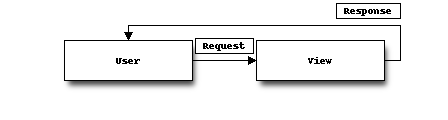
\includegraphics{blockdiag-73065eaf0b801e69ef10fe246919a0006f946ae2.png}\par\end{quote}

Any Python callable can be a view. The only hard and fast requirement
is that it takes the request object (customarily named \code{request}) as
its first argument. This means that a minimalist view is super
simple:

\begin{Verbatim}[commandchars=\\\{\}]
\PYG{k+kn}{from} \PYG{n+nn}{django.http} \PYG{k+kn}{import} \PYG{n}{HttpResponse}

\PYG{k}{def} \PYG{n+nf}{hello\PYGZus{}world}\PYG{p}{(}\PYG{n}{request}\PYG{p}{)}\PYG{p}{:}
    \PYG{k}{return} \PYG{n}{HttpResponse}\PYG{p}{(}\PYG{l+s}{\PYGZdq{}}\PYG{l+s}{Hello, World}\PYG{l+s}{\PYGZdq{}}\PYG{p}{)}
\end{Verbatim}

Of course, like most frameworks, Django also allows you to pass
arguments to the view from the URL. We'll cover this as we build up
our application.


\section{Generic \& Class Based Views}
\label{tutorial/views:http-response}\label{tutorial/views:generic-class-based-views}\begin{itemize}
\item {} 
\href{https://docs.djangoproject.com/en/1.5/topics/class-based-views/generic-display/}{Generic Views} (https://docs.djangoproject.com/en/1.5/topics/class-based-views/generic-display/) have always provided some basic functionality:
render a template, redirect, create or edit a model, etc.

\item {} 
Django 1.3 introduced \href{https://docs.djangoproject.com/en/1.5/topics/class-based-views/}{Class Based Views} (https://docs.djangoproject.com/en/1.5/topics/class-based-views/) (CBV) for the generic views

\item {} 
Provide higher levels of abstraction and composability

\item {} 
Also hide a lot of complexity, which can be confusing for the
newcomer

\item {} 
Luckily the documentation is \textbf{much} better with Django 1.5

\end{itemize}

Django 1.3 introduced class based views, which is what we'll be
focusing on here. Class based views, or CBVs, can eliminate a lot of
boilerplate from your views, especially for things like an edit view
where you want to take different action on a \code{GET} vs \code{POST}. They
give you a lot of power to compose functionality from pieces. The
downside is that this power comes with some added complexity.


\section{Class Based Views}
\label{tutorial/views:class-based-views}
The minimal class based view subclasses \href{https://docs.djangoproject.com/en/1.5/ref/class-based-views/base/\#view}{View} (https://docs.djangoproject.com/en/1.5/ref/class-based-views/base/\#view) and implements methods
for the HTTP methods it supports. Here's the class-based version of
the minimalist ``Hello, World'' view we previously wrote.

\begin{Verbatim}[commandchars=\\\{\}]
\PYG{k+kn}{from} \PYG{n+nn}{django.http} \PYG{k+kn}{import} \PYG{n}{HttpResponse}
\PYG{k+kn}{from} \PYG{n+nn}{django.views.generic} \PYG{k+kn}{import} \PYG{n}{View}

\PYG{k}{class} \PYG{n+nc}{MyView}\PYG{p}{(}\PYG{n}{View}\PYG{p}{)}\PYG{p}{:}

    \PYG{k}{def} \PYG{n+nf}{get}\PYG{p}{(}\PYG{n+nb+bp}{self}\PYG{p}{,} \PYG{n}{request}\PYG{p}{,} \PYG{o}{*}\PYG{n}{args}\PYG{p}{,} \PYG{o}{*}\PYG{o}{*}\PYG{n}{kwargs}\PYG{p}{)}\PYG{p}{:}
        \PYG{k}{return} \PYG{n}{HttpResponse}\PYG{p}{(}\PYG{l+s}{\PYGZdq{}}\PYG{l+s}{Hello, World}\PYG{l+s}{\PYGZdq{}}\PYG{p}{)}
\end{Verbatim}

In a class based view, HTTP methods map to class method names. In this
case, we've defined a handler for \code{GET} requests with the \code{get}
method. Just like the function implementation, it takes \code{request} as
its first argument, and returns an HTTP Response.
\setbox0\vbox{
\begin{minipage}{0.95\linewidth}
\textbf{Permissive Signatures}

\medskip


You may notice that it has a couple of extra arguments in its
signature, compared to the view we saw previously, specifically
\code{*args} and \code{**kwargs}. Class based views were first introduced
as a way to make Django's ``generic'' views more flexible. That meant
they were used in many different contexts, with potentially
different arguments extracted from the URLs. As I've been writing
class based views over the past year, I've continued to write them
with permissive signatures, as I've found they're often useful in
ways I didn't initially expect.
\end{minipage}}
\begin{center}\setlength{\fboxsep}{5pt}\shadowbox{\box0}\end{center}


\section{Listing Contacts}
\label{tutorial/views:listing-contacts}\DUspan{admonition-list-views}{}\DUspan{admonition-edit-views}{}\DUspan{admonition-detail-views}{}
We'll start with a view that presents a list of contacts in the
database.

The basic view implementation is shockingly brief. We can write the
view in just a few lines in the \code{views.py} file in our \code{contacts}
application.

\begin{Verbatim}[commandchars=\\\{\}]
\PYG{k+kn}{from} \PYG{n+nn}{django.views.generic} \PYG{k+kn}{import} \PYG{n}{ListView}

\PYG{k+kn}{from} \PYG{n+nn}{contacts.models} \PYG{k+kn}{import} \PYG{n}{Contact}


\PYG{k}{class} \PYG{n+nc}{ListContactView}\PYG{p}{(}\PYG{n}{ListView}\PYG{p}{)}\PYG{p}{:}

    \PYG{n}{model} \PYG{o}{=} \PYG{n}{Contact}
\end{Verbatim}

The \href{https://docs.djangoproject.com/en/1.5/ref/class-based-views/generic-display/\#listview}{ListView} (https://docs.djangoproject.com/en/1.5/ref/class-based-views/generic-display/\#listview) that we subclass from is itself composed of several
mixins that provide some behavior, and that composition gives us a lot
of power without a lot of code. In this case we set \code{model =
Contact}, which says that this view is going to list \emph{all} the
Contacts in our database.


\section{Defining URLs}
\label{tutorial/views:defining-urls}
The URL configuration tells Django how to match a request's path to
your Python code. Django looks for the URL configuration, defined as
\code{urlpatterns}, in the \code{urls.py} file in your project.

Let's add a URL mapping for our contact list view in
\code{addressbook/urls.py}.

\begin{Verbatim}[commandchars=\\\{\}]
\PYG{k+kn}{from} \PYG{n+nn}{django.conf.urls} \PYG{k+kn}{import} \PYG{n}{patterns}\PYG{p}{,} \PYG{n}{include}\PYG{p}{,} \PYG{n}{url}

\PYG{k+kn}{import} \PYG{n+nn}{contacts.views}


\PYG{n}{urlpatterns} \PYG{o}{=} \PYG{n}{patterns}\PYG{p}{(}\PYG{l+s}{\PYGZsq{}}\PYG{l+s}{\PYGZsq{}}\PYG{p}{,}
    \PYG{n}{url}\PYG{p}{(}\PYG{l+s}{r\PYGZsq{}}\PYG{l+s}{\PYGZca{}\PYGZdl{}}\PYG{l+s}{\PYGZsq{}}\PYG{p}{,} \PYG{n}{contacts}\PYG{o}{.}\PYG{n}{views}\PYG{o}{.}\PYG{n}{ListContactView}\PYG{o}{.}\PYG{n}{as\PYGZus{}view}\PYG{p}{(}\PYG{p}{)}\PYG{p}{,}
        \PYG{n}{name}\PYG{o}{=}\PYG{l+s}{\PYGZsq{}}\PYG{l+s}{contacts\PYGZhy{}list}\PYG{l+s}{\PYGZsq{}}\PYG{p}{,}\PYG{p}{)}\PYG{p}{,}
\PYG{p}{)}
\end{Verbatim}
\begin{itemize}
\item {} 
Use of the \code{url()} function is not strictly required, but I like
it: when you start adding more information to the URL pattern, it
lets you use named parameters, making everything more clear.

\item {} 
The first parameter is a regular expression. Note the trailing
\code{\$}; why might that be important?

\item {} 
The second parameter is the view callable. It can either be the
actual callable (imported manually), or a string describing it. If
it's a string, Django will import the module (up to the final dot),
and then calls the final segment when a request matches.

\item {} 
Note that when we're using a class based view, we \emph{must} use the
real object here, and not the string notation. That's because we
have to call the class method \code{as\_view()}, which returns a wrapper
around our class that Django's URL dispatch can call.

\item {} 
Giving a URL pattern a name allows you to do a reverse lookup

\item {} 
The URL name is useful when linking from one View to another, or
redirecting, as it allows you to manage your URL structure in one
place

\end{itemize}

While the \code{urlpatterns} name \textbf{must} be defined, Django also allows
you to define a few other values in the URL configuration for
exceptional cases. These include \code{handler403}, \code{handler404}, and
\code{handler500}, which tell Django what view to use when an HTTP error
occurs. See the \href{https://docs.djangoproject.com/en/1.5/ref/urls/\#handler403}{Django urlconf documentation} (https://docs.djangoproject.com/en/1.5/ref/urls/\#handler403) for details.

\begin{notice}{note}{URL Configuration Import Errors}

Django loads the URL configuration very early during startup, and
will attempt to import things it finds here. If one of the imports
fails, however, the error message can be somewhat opaque. If your
project stops working with an import-related exception, try to
import the URL configuration in the interactive shell. That usually
makes it clear where the problem lies.
\end{notice}


\section{Creating the Template}
\label{tutorial/views:creating-the-template}\DUspan{admonition-django-templates}{}
Now that we've defined a URL for our list view, we can try it out.
Django includes a server suitable for development purposes that you
can use to easily test your project:

\begin{Verbatim}[commandchars=\\\{\}]
\PYGZdl{} python manage.py runserver
Validating models...

0 errors found
Django version 1.4.3, using settings \PYGZsq{}addressbook.settings\PYGZsq{}
Development server is running at http://127.0.0.1:8000/
Quit the server with CONTROL\PYGZhy{}C.
\end{Verbatim}

If you visit the \code{http://localhost:8000/} in your browser, though,
you'll see an error: \code{TemplateDoesNotExist}.

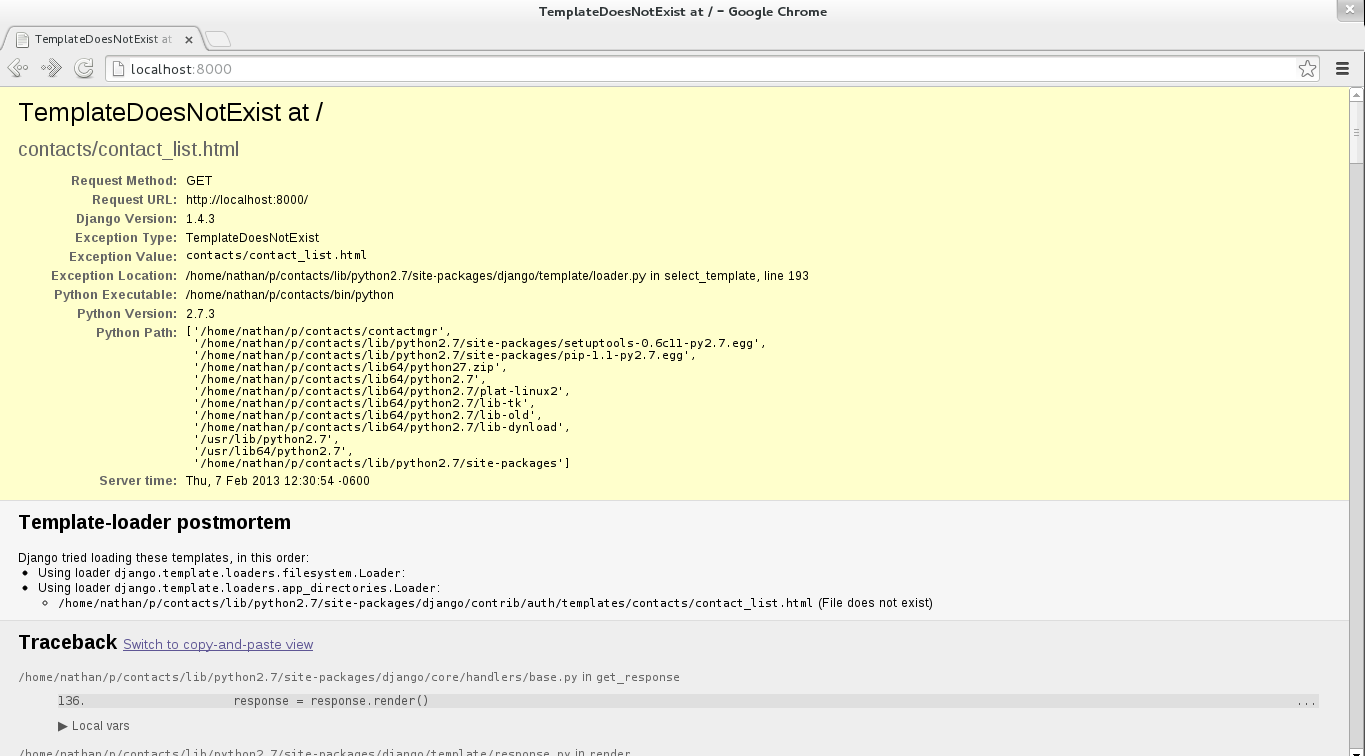
\includegraphics{TemplateDoesNotExist.png}

Most of Django's generic views (such as \code{ListView} which we're
using) have a predefined template name that they expect to find. We
can see in this error message that this view was expecting to find
\code{contact\_list.html}, which is derived from the model name. Let's go
and create that.

By default Django will look for templates in applications, as well as
in directories you specify in \code{settings.TEMPLATE\_DIRS}. The generic
views expect that the templates will be found in a directory named
after the application (in this case \code{contacts}), and the filename
will contain the model name (in this case \code{contact\_list.html}). This
works very well when you're distributing a reusable application: the
consumer can create templates that override the defaults, and they're
clearly stored in a directory associated with the application.

For our purposes, however, we don't need that extra layer of directory
structure, so we'll specify the template to use explicitly, using the
\code{template\_name} property. Let's add that one line to \code{views.py}.

\begin{Verbatim}[commandchars=\\\{\}]
\PYG{k+kn}{from} \PYG{n+nn}{django.views.generic} \PYG{k+kn}{import} \PYG{n}{ListView}

\PYG{k+kn}{from} \PYG{n+nn}{contacts.models} \PYG{k+kn}{import} \PYG{n}{Contact}


\PYG{k}{class} \PYG{n+nc}{ListContactView}\PYG{p}{(}\PYG{n}{ListView}\PYG{p}{)}\PYG{p}{:}

    \PYG{n}{model} \PYG{o}{=} \PYG{n}{Contact}
    \PYG{n}{template\PYGZus{}name} \PYG{o}{=} \PYG{l+s}{\PYGZsq{}}\PYG{l+s}{contact\PYGZus{}list.html}\PYG{l+s}{\PYGZsq{}}
\end{Verbatim}

Create a \code{templates} subdirectory in our \code{contacts} application,
and create \code{contact\_list.html} there.

\begin{Verbatim}[commandchars=\\\{\}]
\PYG{n+nt}{\PYGZlt{}h1}\PYG{n+nt}{\PYGZgt{}}Contacts\PYG{n+nt}{\PYGZlt{}/h1\PYGZgt{}}

\PYG{n+nt}{\PYGZlt{}ul}\PYG{n+nt}{\PYGZgt{}}
  \PYGZob{}\PYGZpc{} for contact in object\PYGZus{}list \PYGZpc{}\PYGZcb{}
    \PYG{n+nt}{\PYGZlt{}li} \PYG{n+na}{class=}\PYG{l+s}{\PYGZdq{}contact\PYGZdq{}}\PYG{n+nt}{\PYGZgt{}}\PYGZob{}\PYGZob{} contact \PYGZcb{}\PYGZcb{}\PYG{n+nt}{\PYGZlt{}/li\PYGZgt{}}
  \PYGZob{}\PYGZpc{} endfor \PYGZpc{}\PYGZcb{}
\PYG{n+nt}{\PYGZlt{}/ul\PYGZgt{}}
\end{Verbatim}

Opening the page in the browser, we should see one contact there, the
one we added earlier through the interactive shell.


\section{Creating Contacts}
\label{tutorial/views:creating-contacts}
Adding information to the database through the interactive shell is
going to get old fast, so let's create a view for adding a new
contact.

Just like the list view, we'll use one of Django's generic views. In
\code{views.py}, we can add the new view:

\begin{Verbatim}[commandchars=\\\{\}]
\PYG{k+kn}{from} \PYG{n+nn}{django.core.urlresolvers} \PYG{k+kn}{import} \PYG{n}{reverse}
\PYG{k+kn}{from} \PYG{n+nn}{django.views.generic} \PYG{k+kn}{import} \PYG{n}{CreateView}
\PYG{o}{.}\PYG{o}{.}\PYG{o}{.}
\PYG{k}{class} \PYG{n+nc}{CreateContactView}\PYG{p}{(}\PYG{n}{CreateView}\PYG{p}{)}\PYG{p}{:}

    \PYG{n}{model} \PYG{o}{=} \PYG{n}{Contact}
    \PYG{n}{template\PYGZus{}name} \PYG{o}{=} \PYG{l+s}{\PYGZsq{}}\PYG{l+s}{edit\PYGZus{}contact.html}\PYG{l+s}{\PYGZsq{}}

    \PYG{k}{def} \PYG{n+nf}{get\PYGZus{}success\PYGZus{}url}\PYG{p}{(}\PYG{n+nb+bp}{self}\PYG{p}{)}\PYG{p}{:}
        \PYG{k}{return} \PYG{n}{reverse}\PYG{p}{(}\PYG{l+s}{\PYGZsq{}}\PYG{l+s}{contacts\PYGZhy{}list}\PYG{l+s}{\PYGZsq{}}\PYG{p}{)}
\end{Verbatim}

Most generic views that do form processing have the concept of the
``success URL'': where to redirect the user when the form is
successfully submitted. The form processing views all adhere to the
practice of POST-redirect-GET for submitting changes, so that
refreshing the final page won't result in form re-submission. You can
either define this as a class property, or override the
\code{get\_success\_url()} method, as we're doing here. In this case we're
using the \code{reverse} function to calculate the URL of the contact
list.
\setbox0\vbox{
\begin{minipage}{0.95\linewidth}
\textbf{Context Variables in Class Based Views}

\medskip


The collection of values available to a template when it's rendered
is referred to as the Context. The Context is a combination of
information supplied by the view and information from \href{https://docs.djangoproject.com/en/1.5/ref/templates/api/\#subclassing-context-requestcontext}{context
processors} (https://docs.djangoproject.com/en/1.5/ref/templates/api/\#subclassing-context-requestcontext).

When you're using built in generic views, it's not obvious what
values are available to the context. With some practice you'll
discover they're pretty consistent -- \code{form}, \code{object}, and
\code{object\_list} are often used -- but that doesn't help when you're
just starting off. Luckily, the documentation for this is much
improved with Django 1.5.

In class based views, the \code{get\_context\_data()} method is used to
add information to the context. If you override this method, you
usually want to accept \code{**kwargs}, and call the super class.
\end{minipage}}
\begin{center}\setlength{\fboxsep}{5pt}\shadowbox{\box0}\end{center}

The template is slightly more involved than the list template, but not
much. Our \code{edit\_contact.html} will look something like this.

\begin{Verbatim}[commandchars=\\\{\}]
\PYGZlt{}h1\PYGZgt{}Add Contact\PYGZlt{}/h1\PYGZgt{}

\PYGZlt{}form action=\PYGZdq{}\PYGZob{}\PYGZpc{} url \PYGZdq{}contacts\PYGZhy{}new\PYGZdq{} \PYGZpc{}\PYGZcb{}\PYGZdq{} method=\PYGZdq{}POST\PYGZdq{}\PYGZgt{}
  \PYGZob{}\PYGZpc{} csrf\PYGZus{}token \PYGZpc{}\PYGZcb{}
  \PYGZlt{}ul\PYGZgt{}
    \PYGZob{}\PYGZob{} form.as\PYGZus{}ul \PYGZcb{}\PYGZcb{}
  \PYGZlt{}/ul\PYGZgt{}
  \PYGZlt{}input id=\PYGZdq{}save\PYGZus{}contact\PYGZdq{} type=\PYGZdq{}submit\PYGZdq{} value=\PYGZdq{}Save\PYGZdq{} /\PYGZgt{}
\PYGZlt{}/form\PYGZgt{}

\PYGZlt{}a href=\PYGZdq{}\PYGZob{}\PYGZpc{} url \PYGZdq{}contacts\PYGZhy{}list\PYGZdq{} \PYGZpc{}\PYGZcb{}\PYGZdq{}\PYGZgt{}back to list\PYGZlt{}/a\PYGZgt{}
\end{Verbatim}

A few things to note:
\begin{itemize}
\item {} 
The \code{form} in the context is the \href{https://docs.djangoproject.com/en/1.5/topics/forms/}{Django Form} (https://docs.djangoproject.com/en/1.5/topics/forms/) for our model.
Since we didn't specify one, Django made one for us. How thoughtful.

\item {} 
If we just write \code{\{\{ form \}\}} we'll get table rows; adding
\code{.as\_ul} formats the inputs for an unordered list. Try \code{.as\_p}
instead to see what you get.

\item {} 
When we output the form, it only includes our fields, not the
surrounding \code{\textless{}form\textgreater{}} tag or the submit button, so we have to add
those.

\item {} 
The \code{\{\% csrf\_token \%\}} tag inserts a hidden input that Django uses
to verify that the request came from your project, and isn't a
forged cross-site request. Try omitting it: you can still access the
page, but when you go to submit the form, you'll get an error.

\item {} 
We're using the \code{url} template tag to generate the link back to
the contact list. Note that \code{contacts-list} is the name of our
view from the URL configuration. By using \code{url} instead of an
explicit path, we don't have to worry about a link breaking. \code{url}
in templates is equivalent to \code{reverse} in Python code.

\end{itemize}

Finally, let's configure the URL by adding the following line to our
\code{urls.py} file:

\begin{Verbatim}[commandchars=\\\{\}]
\PYG{n}{url}\PYG{p}{(}\PYG{l+s}{r\PYGZsq{}}\PYG{l+s}{\PYGZca{}new\PYGZdl{}}\PYG{l+s}{\PYGZsq{}}\PYG{p}{,} \PYG{n}{contacts}\PYG{o}{.}\PYG{n}{views}\PYG{o}{.}\PYG{n}{CreateContactView}\PYG{o}{.}\PYG{n}{as\PYGZus{}view}\PYG{p}{(}\PYG{p}{)}\PYG{p}{,}
    \PYG{n}{name}\PYG{o}{=}\PYG{l+s}{\PYGZsq{}}\PYG{l+s}{contacts\PYGZhy{}new}\PYG{l+s}{\PYGZsq{}}\PYG{p}{,}\PYG{p}{)}\PYG{p}{,}
\end{Verbatim}

You can go to \code{http://localhost:8000/new} to create new contacts


\section{Testing Your Views}
\label{tutorial/views:testing-your-views}\DUspan{admonition-test-client-requestfactory}{}\DUspan{admonition-test-client-vs-requestfactory}{}
So far our views have been pretty minimal: they leverage Django's
generic views, and contain very little of our own code or logic. One
perspective is that this is how it should be: a view takes a request,
and returns a response, delegating the issue of validating input to
forms, and business logic to model methods. This is a perspective that
I subscribe to. The less logic contained in views, the better.

However, there is code in views that should be tested, either by unit
tests or integration tests. The distinction is important: unit tests
are focused on testing a single unit of functionality. When you're
writing a unit test, the assumption is that everything else has its
own tests and is working properly. Integration tests attempt to test
the system from end to end, so you can ensure that the points of
integration are functioning properly. Most systems have both.

Django has two tools that are helpful for writing unit tests for
views: the Test \href{https://docs.djangoproject.com/en/1.5/topics/testing/overview/\#module-django.test.client}{Client} (https://docs.djangoproject.com/en/1.5/topics/testing/overview/\#module-django.test.client) and the \href{https://docs.djangoproject.com/en/1.5/topics/testing/advanced/\#django.test.client.RequestFactory}{RequestFactory} (https://docs.djangoproject.com/en/1.5/topics/testing/advanced/\#django.test.client.RequestFactory). They have similar
APIs, but approach things differently. The \code{TestClient} takes a URL
to retrieve, and resolves it against your project's URL configuration.
It then creates a test request, and passes that request through your
view, returning the Response. The fact that it requires you to specify
the URL ties your test to the URL configuration of your project.

The \code{RequestFactory} has the same API: you specify the URL you want
to retrieve and any parameters or form data. But it doesn't actually
resolve that URL: it just returns the Request object. You can then
manually pass it to your view and test the result.

In practice, RequestFactory tests are usually somewhat faster than the
TestClient. This isn't a big deal when you have five tests, but it is
when you have 500 or 5,000. Let's look at the same test written with
each tool.

\begin{Verbatim}[commandchars=\\\{\}]
\PYG{k+kn}{from} \PYG{n+nn}{django.test.client} \PYG{k+kn}{import} \PYG{n}{Client}
\PYG{k+kn}{from} \PYG{n+nn}{django.test.client} \PYG{k+kn}{import} \PYG{n}{RequestFactory}
\PYG{o}{.}\PYG{o}{.}\PYG{o}{.}
\PYG{k+kn}{from} \PYG{n+nn}{contacts.views} \PYG{k+kn}{import} \PYG{n}{ListContactView}
\PYG{o}{.}\PYG{o}{.}\PYG{o}{.}
\PYG{k}{class} \PYG{n+nc}{ContactListViewTests}\PYG{p}{(}\PYG{n}{TestCase}\PYG{p}{)}\PYG{p}{:}
    \PYG{l+s+sd}{\PYGZdq{}\PYGZdq{}\PYGZdq{}Contact list view tests.\PYGZdq{}\PYGZdq{}\PYGZdq{}}

    \PYG{k}{def} \PYG{n+nf}{test\PYGZus{}contacts\PYGZus{}in\PYGZus{}the\PYGZus{}context}\PYG{p}{(}\PYG{n+nb+bp}{self}\PYG{p}{)}\PYG{p}{:}

        \PYG{n}{client} \PYG{o}{=} \PYG{n}{Client}\PYG{p}{(}\PYG{p}{)}
        \PYG{n}{response} \PYG{o}{=} \PYG{n}{client}\PYG{o}{.}\PYG{n}{get}\PYG{p}{(}\PYG{l+s}{\PYGZsq{}}\PYG{l+s}{/}\PYG{l+s}{\PYGZsq{}}\PYG{p}{)}

        \PYG{n+nb+bp}{self}\PYG{o}{.}\PYG{n}{assertEquals}\PYG{p}{(}\PYG{n+nb}{list}\PYG{p}{(}\PYG{n}{response}\PYG{o}{.}\PYG{n}{context}\PYG{p}{[}\PYG{l+s}{\PYGZsq{}}\PYG{l+s}{object\PYGZus{}list}\PYG{l+s}{\PYGZsq{}}\PYG{p}{]}\PYG{p}{)}\PYG{p}{,} \PYG{p}{[}\PYG{p}{]}\PYG{p}{)}

        \PYG{n}{Contact}\PYG{o}{.}\PYG{n}{objects}\PYG{o}{.}\PYG{n}{create}\PYG{p}{(}\PYG{n}{first\PYGZus{}name}\PYG{o}{=}\PYG{l+s}{\PYGZsq{}}\PYG{l+s}{foo}\PYG{l+s}{\PYGZsq{}}\PYG{p}{,} \PYG{n}{last\PYGZus{}name}\PYG{o}{=}\PYG{l+s}{\PYGZsq{}}\PYG{l+s}{bar}\PYG{l+s}{\PYGZsq{}}\PYG{p}{)}
        \PYG{n}{response} \PYG{o}{=} \PYG{n}{client}\PYG{o}{.}\PYG{n}{get}\PYG{p}{(}\PYG{l+s}{\PYGZsq{}}\PYG{l+s}{/}\PYG{l+s}{\PYGZsq{}}\PYG{p}{)}
        \PYG{n+nb+bp}{self}\PYG{o}{.}\PYG{n}{assertEquals}\PYG{p}{(}\PYG{n}{response}\PYG{o}{.}\PYG{n}{context}\PYG{p}{[}\PYG{l+s}{\PYGZsq{}}\PYG{l+s}{object\PYGZus{}list}\PYG{l+s}{\PYGZsq{}}\PYG{p}{]}\PYG{o}{.}\PYG{n}{count}\PYG{p}{(}\PYG{p}{)}\PYG{p}{,} \PYG{l+m+mi}{1}\PYG{p}{)}

    \PYG{k}{def} \PYG{n+nf}{test\PYGZus{}contacts\PYGZus{}in\PYGZus{}the\PYGZus{}context\PYGZus{}request\PYGZus{}factory}\PYG{p}{(}\PYG{n+nb+bp}{self}\PYG{p}{)}\PYG{p}{:}

        \PYG{n}{factory} \PYG{o}{=} \PYG{n}{RequestFactory}\PYG{p}{(}\PYG{p}{)}
        \PYG{n}{request} \PYG{o}{=} \PYG{n}{factory}\PYG{o}{.}\PYG{n}{get}\PYG{p}{(}\PYG{l+s}{\PYGZsq{}}\PYG{l+s}{/}\PYG{l+s}{\PYGZsq{}}\PYG{p}{)}

        \PYG{n}{response} \PYG{o}{=} \PYG{n}{ListContactView}\PYG{o}{.}\PYG{n}{as\PYGZus{}view}\PYG{p}{(}\PYG{p}{)}\PYG{p}{(}\PYG{n}{request}\PYG{p}{)}

        \PYG{n+nb+bp}{self}\PYG{o}{.}\PYG{n}{assertEquals}\PYG{p}{(}\PYG{n+nb}{list}\PYG{p}{(}\PYG{n}{response}\PYG{o}{.}\PYG{n}{context\PYGZus{}data}\PYG{p}{[}\PYG{l+s}{\PYGZsq{}}\PYG{l+s}{object\PYGZus{}list}\PYG{l+s}{\PYGZsq{}}\PYG{p}{]}\PYG{p}{)}\PYG{p}{,} \PYG{p}{[}\PYG{p}{]}\PYG{p}{)}

        \PYG{n}{Contact}\PYG{o}{.}\PYG{n}{objects}\PYG{o}{.}\PYG{n}{create}\PYG{p}{(}\PYG{n}{first\PYGZus{}name}\PYG{o}{=}\PYG{l+s}{\PYGZsq{}}\PYG{l+s}{foo}\PYG{l+s}{\PYGZsq{}}\PYG{p}{,} \PYG{n}{last\PYGZus{}name}\PYG{o}{=}\PYG{l+s}{\PYGZsq{}}\PYG{l+s}{bar}\PYG{l+s}{\PYGZsq{}}\PYG{p}{)}
        \PYG{n}{response} \PYG{o}{=} \PYG{n}{ListContactView}\PYG{o}{.}\PYG{n}{as\PYGZus{}view}\PYG{p}{(}\PYG{p}{)}\PYG{p}{(}\PYG{n}{request}\PYG{p}{)}
        \PYG{n+nb+bp}{self}\PYG{o}{.}\PYG{n}{assertEquals}\PYG{p}{(}\PYG{n}{response}\PYG{o}{.}\PYG{n}{context\PYGZus{}data}\PYG{p}{[}\PYG{l+s}{\PYGZsq{}}\PYG{l+s}{object\PYGZus{}list}\PYG{l+s}{\PYGZsq{}}\PYG{p}{]}\PYG{o}{.}\PYG{n}{count}\PYG{p}{(}\PYG{p}{)}\PYG{p}{,} \PYG{l+m+mi}{1}\PYG{p}{)}
\end{Verbatim}


\section{Integration Tests}
\label{tutorial/views:integration-tests}\DUspan{admonition-live-server-tests}{}
Django 1.4 adds a new \code{TestCase} base class, the
\href{https://docs.djangoproject.com/en/1.5/topics/testing/overview/\#liveservertestcase}{LiveServerTestCase} (https://docs.djangoproject.com/en/1.5/topics/testing/overview/\#liveservertestcase). This is very much what it sounds like: a test
case that runs against a live server. By default Django will start the
development server for you when it runs these tests, but they can also
be run against another server.

\href{http://seleniumhq.org/}{Selenium} (http://seleniumhq.org/) is a tool for writing tests that drive a web browser, and
that's what we'll use for our integration tests. By using Selenium,
you're able to automate different browers (Chrome, Firefox, etc), and
interact with your full application much as the user would. Before
writing tests to use it, we'll need to install the Python implementation.

\begin{Verbatim}[commandchars=\\\{\}]
(tutorial)\PYGZdl{} pip install selenium
\end{Verbatim}

We're going to write a couple of tests for our views:
\begin{itemize}
\item {} 
one that creates a Contact and makes sure it's listed

\item {} 
one that makes sure our ``add contact'' link is visible and linked on
the list page

\item {} 
and one that actually exercises the add contact form, filling it in
and submitting it.

\end{itemize}

\begin{Verbatim}[commandchars=\\\{\}]
\PYG{k+kn}{from} \PYG{n+nn}{django.test} \PYG{k+kn}{import} \PYG{n}{LiveServerTestCase}
\PYG{k+kn}{from} \PYG{n+nn}{selenium.webdriver.firefox.webdriver} \PYG{k+kn}{import} \PYG{n}{WebDriver}
\PYG{o}{.}\PYG{o}{.}\PYG{o}{.}
\PYG{k}{class} \PYG{n+nc}{ContactListIntegrationTests}\PYG{p}{(}\PYG{n}{LiveServerTestCase}\PYG{p}{)}\PYG{p}{:}

    \PYG{n+nd}{@classmethod}
    \PYG{k}{def} \PYG{n+nf}{setUpClass}\PYG{p}{(}\PYG{n}{cls}\PYG{p}{)}\PYG{p}{:}
        \PYG{n}{cls}\PYG{o}{.}\PYG{n}{selenium} \PYG{o}{=} \PYG{n}{WebDriver}\PYG{p}{(}\PYG{p}{)}
        \PYG{n+nb}{super}\PYG{p}{(}\PYG{n}{ContactListIntegrationTests}\PYG{p}{,} \PYG{n}{cls}\PYG{p}{)}\PYG{o}{.}\PYG{n}{setUpClass}\PYG{p}{(}\PYG{p}{)}

    \PYG{n+nd}{@classmethod}
    \PYG{k}{def} \PYG{n+nf}{tearDownClass}\PYG{p}{(}\PYG{n}{cls}\PYG{p}{)}\PYG{p}{:}
        \PYG{n}{cls}\PYG{o}{.}\PYG{n}{selenium}\PYG{o}{.}\PYG{n}{quit}\PYG{p}{(}\PYG{p}{)}
        \PYG{n+nb}{super}\PYG{p}{(}\PYG{n}{ContactListIntegrationTests}\PYG{p}{,} \PYG{n}{cls}\PYG{p}{)}\PYG{o}{.}\PYG{n}{tearDownClass}\PYG{p}{(}\PYG{p}{)}

    \PYG{k}{def} \PYG{n+nf}{test\PYGZus{}contact\PYGZus{}listed}\PYG{p}{(}\PYG{n+nb+bp}{self}\PYG{p}{)}\PYG{p}{:}

        \PYG{c}{\PYGZsh{} create a test contact}
        \PYG{n}{Contact}\PYG{o}{.}\PYG{n}{objects}\PYG{o}{.}\PYG{n}{create}\PYG{p}{(}\PYG{n}{first\PYGZus{}name}\PYG{o}{=}\PYG{l+s}{\PYGZsq{}}\PYG{l+s}{foo}\PYG{l+s}{\PYGZsq{}}\PYG{p}{,} \PYG{n}{last\PYGZus{}name}\PYG{o}{=}\PYG{l+s}{\PYGZsq{}}\PYG{l+s}{bar}\PYG{l+s}{\PYGZsq{}}\PYG{p}{)}

        \PYG{c}{\PYGZsh{} make sure it\PYGZsq{}s listed as \PYGZlt{}first\PYGZgt{} \PYGZlt{}last\PYGZgt{} on the list}
        \PYG{n+nb+bp}{self}\PYG{o}{.}\PYG{n}{selenium}\PYG{o}{.}\PYG{n}{get}\PYG{p}{(}\PYG{l+s}{\PYGZsq{}}\PYG{l+s+si}{\PYGZpc{}s}\PYG{l+s+si}{\PYGZpc{}s}\PYG{l+s}{\PYGZsq{}} \PYG{o}{\PYGZpc{}} \PYG{p}{(}\PYG{n+nb+bp}{self}\PYG{o}{.}\PYG{n}{live\PYGZus{}server\PYGZus{}url}\PYG{p}{,} \PYG{l+s}{\PYGZsq{}}\PYG{l+s}{/}\PYG{l+s}{\PYGZsq{}}\PYG{p}{)}\PYG{p}{)}
        \PYG{n+nb+bp}{self}\PYG{o}{.}\PYG{n}{assertEqual}\PYG{p}{(}
            \PYG{n+nb+bp}{self}\PYG{o}{.}\PYG{n}{selenium}\PYG{o}{.}\PYG{n}{find\PYGZus{}elements\PYGZus{}by\PYGZus{}css\PYGZus{}selector}\PYG{p}{(}\PYG{l+s}{\PYGZsq{}}\PYG{l+s}{.contact}\PYG{l+s}{\PYGZsq{}}\PYG{p}{)}\PYG{p}{[}\PYG{l+m+mi}{0}\PYG{p}{]}\PYG{o}{.}\PYG{n}{text}\PYG{p}{,}
            \PYG{l+s}{\PYGZsq{}}\PYG{l+s}{foo bar}\PYG{l+s}{\PYGZsq{}}
        \PYG{p}{)}

    \PYG{k}{def} \PYG{n+nf}{test\PYGZus{}add\PYGZus{}contact\PYGZus{}linked}\PYG{p}{(}\PYG{n+nb+bp}{self}\PYG{p}{)}\PYG{p}{:}

        \PYG{n+nb+bp}{self}\PYG{o}{.}\PYG{n}{selenium}\PYG{o}{.}\PYG{n}{get}\PYG{p}{(}\PYG{l+s}{\PYGZsq{}}\PYG{l+s+si}{\PYGZpc{}s}\PYG{l+s+si}{\PYGZpc{}s}\PYG{l+s}{\PYGZsq{}} \PYG{o}{\PYGZpc{}} \PYG{p}{(}\PYG{n+nb+bp}{self}\PYG{o}{.}\PYG{n}{live\PYGZus{}server\PYGZus{}url}\PYG{p}{,} \PYG{l+s}{\PYGZsq{}}\PYG{l+s}{/}\PYG{l+s}{\PYGZsq{}}\PYG{p}{)}\PYG{p}{)}
        \PYG{n+nb+bp}{self}\PYG{o}{.}\PYG{n}{assert\PYGZus{}}\PYG{p}{(}
            \PYG{n+nb+bp}{self}\PYG{o}{.}\PYG{n}{selenium}\PYG{o}{.}\PYG{n}{find\PYGZus{}element\PYGZus{}by\PYGZus{}link\PYGZus{}text}\PYG{p}{(}\PYG{l+s}{\PYGZsq{}}\PYG{l+s}{add contact}\PYG{l+s}{\PYGZsq{}}\PYG{p}{)}
        \PYG{p}{)}

    \PYG{k}{def} \PYG{n+nf}{test\PYGZus{}add\PYGZus{}contact}\PYG{p}{(}\PYG{n+nb+bp}{self}\PYG{p}{)}\PYG{p}{:}

        \PYG{n+nb+bp}{self}\PYG{o}{.}\PYG{n}{selenium}\PYG{o}{.}\PYG{n}{get}\PYG{p}{(}\PYG{l+s}{\PYGZsq{}}\PYG{l+s+si}{\PYGZpc{}s}\PYG{l+s+si}{\PYGZpc{}s}\PYG{l+s}{\PYGZsq{}} \PYG{o}{\PYGZpc{}} \PYG{p}{(}\PYG{n+nb+bp}{self}\PYG{o}{.}\PYG{n}{live\PYGZus{}server\PYGZus{}url}\PYG{p}{,} \PYG{l+s}{\PYGZsq{}}\PYG{l+s}{/}\PYG{l+s}{\PYGZsq{}}\PYG{p}{)}\PYG{p}{)}
        \PYG{n+nb+bp}{self}\PYG{o}{.}\PYG{n}{selenium}\PYG{o}{.}\PYG{n}{find\PYGZus{}element\PYGZus{}by\PYGZus{}link\PYGZus{}text}\PYG{p}{(}\PYG{l+s}{\PYGZsq{}}\PYG{l+s}{add contact}\PYG{l+s}{\PYGZsq{}}\PYG{p}{)}\PYG{o}{.}\PYG{n}{click}\PYG{p}{(}\PYG{p}{)}

        \PYG{n+nb+bp}{self}\PYG{o}{.}\PYG{n}{selenium}\PYG{o}{.}\PYG{n}{find\PYGZus{}element\PYGZus{}by\PYGZus{}id}\PYG{p}{(}\PYG{l+s}{\PYGZsq{}}\PYG{l+s}{id\PYGZus{}first\PYGZus{}name}\PYG{l+s}{\PYGZsq{}}\PYG{p}{)}\PYG{o}{.}\PYG{n}{send\PYGZus{}keys}\PYG{p}{(}\PYG{l+s}{\PYGZsq{}}\PYG{l+s}{test}\PYG{l+s}{\PYGZsq{}}\PYG{p}{)}
        \PYG{n+nb+bp}{self}\PYG{o}{.}\PYG{n}{selenium}\PYG{o}{.}\PYG{n}{find\PYGZus{}element\PYGZus{}by\PYGZus{}id}\PYG{p}{(}\PYG{l+s}{\PYGZsq{}}\PYG{l+s}{id\PYGZus{}last\PYGZus{}name}\PYG{l+s}{\PYGZsq{}}\PYG{p}{)}\PYG{o}{.}\PYG{n}{send\PYGZus{}keys}\PYG{p}{(}\PYG{l+s}{\PYGZsq{}}\PYG{l+s}{contact}\PYG{l+s}{\PYGZsq{}}\PYG{p}{)}
        \PYG{n+nb+bp}{self}\PYG{o}{.}\PYG{n}{selenium}\PYG{o}{.}\PYG{n}{find\PYGZus{}element\PYGZus{}by\PYGZus{}id}\PYG{p}{(}\PYG{l+s}{\PYGZsq{}}\PYG{l+s}{id\PYGZus{}email}\PYG{l+s}{\PYGZsq{}}\PYG{p}{)}\PYG{o}{.}\PYG{n}{send\PYGZus{}keys}\PYG{p}{(}\PYG{l+s}{\PYGZsq{}}\PYG{l+s}{test@example.com}\PYG{l+s}{\PYGZsq{}}\PYG{p}{)}

        \PYG{n+nb+bp}{self}\PYG{o}{.}\PYG{n}{selenium}\PYG{o}{.}\PYG{n}{find\PYGZus{}element\PYGZus{}by\PYGZus{}id}\PYG{p}{(}\PYG{l+s}{\PYGZdq{}}\PYG{l+s}{save\PYGZus{}contact}\PYG{l+s}{\PYGZdq{}}\PYG{p}{)}\PYG{o}{.}\PYG{n}{click}\PYG{p}{(}\PYG{p}{)}
        \PYG{n+nb+bp}{self}\PYG{o}{.}\PYG{n}{assertEqual}\PYG{p}{(}
            \PYG{n+nb+bp}{self}\PYG{o}{.}\PYG{n}{selenium}\PYG{o}{.}\PYG{n}{find\PYGZus{}elements\PYGZus{}by\PYGZus{}css\PYGZus{}selector}\PYG{p}{(}\PYG{l+s}{\PYGZsq{}}\PYG{l+s}{.contact}\PYG{l+s}{\PYGZsq{}}\PYG{p}{)}\PYG{p}{[}\PYG{o}{\PYGZhy{}}\PYG{l+m+mi}{1}\PYG{p}{]}\PYG{o}{.}\PYG{n}{text}\PYG{p}{,}
            \PYG{l+s}{\PYGZsq{}}\PYG{l+s}{test contact}\PYG{l+s}{\PYGZsq{}}
        \PYG{p}{)}
\end{Verbatim}

Note that Selenium allows us to find elements in the page, inspect
their state, click them, and send keystrokes. In short, it's like
we're controlling the browser. In fact, if you run the tests now,
you'll see a browser open when the tests run.

In our example we're using CSS Selectors to locate elements in the
DOM, but you can also use Xpath. For many people it's a matter of
preference, but I've found that using CSS Selectors is often less
brittle: if I change the markup, I'm likely to leave classes on
important elements in place, even if their relative position in the
DOM changes.


\section{Review}
\label{tutorial/views:review}\begin{itemize}
\item {} 
Views take an \href{https://docs.djangoproject.com/en/1.5/ref/request-response/\#httprequest-objects}{HttpRequest} (https://docs.djangoproject.com/en/1.5/ref/request-response/\#httprequest-objects) and turn it into an \href{https://docs.djangoproject.com/en/1.5/ref/request-response/\#httpresponse-objects}{HttpResponse} (https://docs.djangoproject.com/en/1.5/ref/request-response/\#httpresponse-objects)

\item {} 
Generic class-based views introduced with Django 1.3

\item {} 
These let you create reusable, composable views

\item {} 
URLs are defined in \code{urls.py} in your project

\item {} 
Naming URLs lets you calculate the URL to a view

\item {} 
\href{https://docs.djangoproject.com/en/1.5/topics/testing/advanced/\#django.test.client.RequestFactory}{RequestFactory} (https://docs.djangoproject.com/en/1.5/topics/testing/advanced/\#django.test.client.RequestFactory) creates Requests for testing Views
with

\item {} 
\href{https://docs.djangoproject.com/en/1.5/topics/testing/overview/\#liveservertestcase}{LiveServerTestCase} (https://docs.djangoproject.com/en/1.5/topics/testing/overview/\#liveservertestcase) provides basis for writing integration tests

\end{itemize}


\chapter{Using Static Assets}
\label{tutorial/static::doc}\label{tutorial/static:using-static-assets}\label{tutorial/static:selenium}
Now that we have a basic application where we can add contacts and
list them, it's reasonable to think about how we'd make this look more
appealing. Most modern web applications are a combination of server
side code/views, and client side, static assets, such as JavaScript
and CSS. Regardless of whether you choose JavaScript or CoffeeScript,
CSS or SASS, Django provides support for integrating static assets
into your project.


\section{Adding Static Files}
\label{tutorial/static:adding-static-files}
Django distinguishes between ``static'' and ``media'' files. The former
are static assets included with your app or project. The latter are
files uploaded by users using one of the file storage backends. Django
includes a contrib app, \code{django.contrib.staticfiles} for managing
static files and, importantly, generating the URLs to them. You could,
of course, simply hard code the URLs to your static assets, and that'd
probably work for a while. But if you want to move your static assets
to their own server, or to a CDN, using generated URLs let's you make
that change without needing to update your templates.
\code{django.contrib.staticfiles} is enabled by default when you create a
new project, so you can just start using it.

We're going to add \href{http://getbootstrap.com}{Bootstrap} (http://getbootstrap.com) to our project for some basic styling.
You can download the Bootstrap files from its website,
\href{http://getbootstrap.com}{http://getbootstrap.com}.

Django supports adding static files at both the application and
project level. Where you add them sort of depends on how tied to your
specific assembly of apps they are. That is, are they reusable for
anyone using your app, or are they specific to your particular
deployment?

App specific static files are stored in the \code{static} subdirectory
within the app. Django will also look in any directories listed in the
\code{STATICFILES\_DIRS} setting. Let's update our project settings to
specify a static files directory.

\begin{Verbatim}[commandchars=\\\{\}]
\PYG{k+kn}{import} \PYG{n+nn}{os.path}
\PYG{o}{.}\PYG{o}{.}\PYG{o}{.}
\PYG{c}{\PYGZsh{} Additional locations of static files}
\PYG{n}{STATICFILES\PYGZus{}DIRS} \PYG{o}{=} \PYG{p}{(}
    \PYG{c}{\PYGZsh{} Put strings here, like \PYGZdq{}/home/html/static\PYGZdq{} or \PYGZdq{}C:/www/django/static\PYGZdq{}.}
    \PYG{c}{\PYGZsh{} Always use forward slashes, even on Windows.}
    \PYG{c}{\PYGZsh{} Don\PYGZsq{}t forget to use absolute paths, not relative paths.}
    \PYG{n}{os}\PYG{o}{.}\PYG{n}{path}\PYG{o}{.}\PYG{n}{join}\PYG{p}{(}
        \PYG{n}{os}\PYG{o}{.}\PYG{n}{path}\PYG{o}{.}\PYG{n}{dirname}\PYG{p}{(}\PYG{n}{\PYGZus{}\PYGZus{}file\PYGZus{}\PYGZus{}}\PYG{p}{)}\PYG{p}{,}
        \PYG{l+s}{\PYGZsq{}}\PYG{l+s}{static}\PYG{l+s}{\PYGZsq{}}\PYG{p}{,}
    \PYG{p}{)}\PYG{p}{,}
\PYG{p}{)}
\end{Verbatim}

Note that we use \code{os.path} to construct the absolute path. This
ensures Django can locate the files unambiguously.

Let's go ahead and create the static directory in our project and
unpack Bootstrap into it.

\begin{Verbatim}[commandchars=\\\{\}]
(tutorial)\PYGZdl{} mkdir addressbook/static
(tutorial)\PYGZdl{} cd addressbook/static
(tutorial)\PYGZdl{} unzip \PYGZti{}/Downloads/bootstrap.zip
Archive:  /Users/nathan/Downloads/bootstrap.zip
  creating: bootstrap/
  creating: bootstrap/css/
 inflating: bootstrap/css/bootstrap\PYGZhy{}responsive.css
 inflating: bootstrap/css/bootstrap\PYGZhy{}responsive.min.css
 inflating: bootstrap/css/bootstrap.css
 inflating: bootstrap/css/bootstrap.min.css
  creating: bootstrap/img/
 inflating: bootstrap/img/glyphicons\PYGZhy{}halflings\PYGZhy{}white.png
 inflating: bootstrap/img/glyphicons\PYGZhy{}halflings.png
  creating: bootstrap/js/
 inflating: bootstrap/js/bootstrap.js
 inflating: bootstrap/js/bootstrap.min.js
\end{Verbatim}


\section{Referring to Static Files in Templates}
\label{tutorial/static:referring-to-static-files-in-templates}
The Django staticfiles app includes a \href{https://docs.djangoproject.com/en/1.5/ref/templates/builtins/}{template tag} (https://docs.djangoproject.com/en/1.5/ref/templates/builtins/) that make it
easy to refer to static files within your templates. You load template
tag libraries using the \code{load} tag.

\begin{Verbatim}[commandchars=\\\{\}]
\PYGZob{}\PYGZpc{} load staticfiles \PYGZpc{}\PYGZcb{}
\end{Verbatim}

After loading the static files library, you can refer to the file
using the \code{static} tag.

\begin{Verbatim}[commandchars=\\\{\}]
\PYGZlt{}link href=\PYGZdq{}\PYGZob{}\PYGZpc{} static \PYGZsq{}bootstrap/css/bootstrap.min.css\PYGZsq{} \PYGZpc{}\PYGZcb{}\PYGZdq{}
      rel=\PYGZdq{}stylesheet\PYGZdq{} media=\PYGZdq{}screen\PYGZdq{}\PYGZgt{}
\end{Verbatim}

Note that the path we specify is \emph{relative} to the static files
directory. Django is going to join this path with the \code{STATIC\_URL}
setting to generate the actual URL to use.

The \href{https://docs.djangoproject.com/en/1.5/ref/settings/\#std:setting-STATIC\_URL}{STATIC\_URL setting} (https://docs.djangoproject.com/en/1.5/ref/settings/\#std:setting-STATIC\_URL) tells Django what the root URL for your
static files is. By default it's set to \code{/static/}.


\section{Simple Template Inclusion}
\label{tutorial/static:static-url-setting}\label{tutorial/static:simple-template-inclusion}
We want to add the Boostrap CSS to all of our templates, but we'd like
to avoid repeating ourself: if we add it to each template
individually, when we want to make changes (for example, to add
another stylesheet) we have to make them to all the files. To solve
this, we'll create a base template that the others will inherit from.

Let's create \code{base.html} in the \code{templates} directory of our
\code{contacts} app.

\begin{Verbatim}[commandchars=\\\{\}]
\PYGZob{}\PYGZpc{} load staticfiles \PYGZpc{}\PYGZcb{}
\PYGZlt{}html\PYGZgt{}
  \PYGZlt{}head\PYGZgt{}
    \PYGZlt{}link href=\PYGZdq{}\PYGZob{}\PYGZpc{} static \PYGZsq{}bootstrap/css/bootstrap.min.css\PYGZsq{} \PYGZpc{}\PYGZcb{}\PYGZdq{}
          rel=\PYGZdq{}stylesheet\PYGZdq{} media=\PYGZdq{}screen\PYGZdq{}\PYGZgt{}
  \PYGZlt{}/head\PYGZgt{}

  \PYGZlt{}body\PYGZgt{}
    \PYGZob{}\PYGZpc{} block content \PYGZpc{}\PYGZcb{}
    \PYGZob{}\PYGZpc{} endblock \PYGZpc{}\PYGZcb{}

    \PYGZlt{}script src=\PYGZdq{}\PYGZob{}\PYGZpc{} static \PYGZsq{}bootstrap/js/bootstrap.min.js\PYGZsq{} \PYGZpc{}\PYGZcb{}\PYGZdq{}\PYGZgt{}\PYGZlt{}/script\PYGZgt{}
  \PYGZlt{}/body\PYGZgt{}
\PYGZlt{}/html\PYGZgt{}
\end{Verbatim}

\code{base.html} defines the common structure for our pages, and includes
a \code{block} tag, which other templates can fill in.

We'll update \code{contact\_list.html} to extend from \code{base.html} and
fill in the \code{content} block.

\begin{Verbatim}[commandchars=\\\{\}]
\PYGZob{}\PYGZpc{} extends \PYGZdq{}base.html\PYGZdq{} \PYGZpc{}\PYGZcb{}

\PYGZob{}\PYGZpc{} block content \PYGZpc{}\PYGZcb{}
\PYGZlt{}h1\PYGZgt{}Contacts\PYGZlt{}/h1\PYGZgt{}

\PYGZlt{}ul\PYGZgt{}
  \PYGZob{}\PYGZpc{} for contact in object\PYGZus{}list \PYGZpc{}\PYGZcb{}
    \PYGZlt{}li class=\PYGZdq{}contact\PYGZdq{}\PYGZgt{}\PYGZob{}\PYGZob{} contact \PYGZcb{}\PYGZcb{}\PYGZlt{}/li\PYGZgt{}
  \PYGZob{}\PYGZpc{} endfor \PYGZpc{}\PYGZcb{}
\PYGZlt{}/ul\PYGZgt{}

\PYGZlt{}a href=\PYGZdq{}\PYGZob{}\PYGZpc{} url \PYGZdq{}contacts\PYGZhy{}new\PYGZdq{} \PYGZpc{}\PYGZcb{}\PYGZdq{}\PYGZgt{}add contact\PYGZlt{}/a\PYGZgt{}
\PYGZob{}\PYGZpc{} endblock \PYGZpc{}\PYGZcb{}
\end{Verbatim}


\section{Serving Static Files}
\label{tutorial/static:serving-static-files}
We've told Django where we store our static files, and we've told it
what URL structure to use, but we haven't actually connected the two
together. Django doesn't serve static files by default, and for good
reason: using an application server to serve static resources is going
to be ineffecient, at best. The Django documentation on \href{https://docs.djangoproject.com/en/1.5/howto/static-files/deployment/}{deploying
static files} (https://docs.djangoproject.com/en/1.5/howto/static-files/deployment/) does a good job of walking through the options for
getting your static files onto your CDN or static file server.

For development, however, it's convenient to do it all with one
process, so there's a helper. We'll update our \code{addressbook/urls.py}
file to include the \code{staticfiles\_urlpatterns} helper.

\begin{Verbatim}[commandchars=\\\{\}]
\PYG{k+kn}{from} \PYG{n+nn}{django.conf.urls} \PYG{k+kn}{import} \PYG{n}{patterns}\PYG{p}{,} \PYG{n}{include}\PYG{p}{,} \PYG{n}{url}
\PYG{k+kn}{from} \PYG{n+nn}{django.contrib.staticfiles.urls} \PYG{k+kn}{import} \PYG{n}{staticfiles\PYGZus{}urlpatterns}

\PYG{k+kn}{import} \PYG{n+nn}{contacts.views}


\PYG{n}{urlpatterns} \PYG{o}{=} \PYG{n}{patterns}\PYG{p}{(}\PYG{l+s}{\PYGZsq{}}\PYG{l+s}{\PYGZsq{}}\PYG{p}{,}
    \PYG{n}{url}\PYG{p}{(}\PYG{l+s}{r\PYGZsq{}}\PYG{l+s}{\PYGZca{}\PYGZdl{}}\PYG{l+s}{\PYGZsq{}}\PYG{p}{,} \PYG{n}{contacts}\PYG{o}{.}\PYG{n}{views}\PYG{o}{.}\PYG{n}{ListContactView}\PYG{o}{.}\PYG{n}{as\PYGZus{}view}\PYG{p}{(}\PYG{p}{)}\PYG{p}{,}
        \PYG{n}{name}\PYG{o}{=}\PYG{l+s}{\PYGZsq{}}\PYG{l+s}{contacts\PYGZhy{}list}\PYG{l+s}{\PYGZsq{}}\PYG{p}{,}\PYG{p}{)}\PYG{p}{,}
    \PYG{n}{url}\PYG{p}{(}\PYG{l+s}{r\PYGZsq{}}\PYG{l+s}{\PYGZca{}new\PYGZdl{}}\PYG{l+s}{\PYGZsq{}}\PYG{p}{,} \PYG{n}{contacts}\PYG{o}{.}\PYG{n}{views}\PYG{o}{.}\PYG{n}{CreateContactView}\PYG{o}{.}\PYG{n}{as\PYGZus{}view}\PYG{p}{(}\PYG{p}{)}\PYG{p}{,}
        \PYG{n}{name}\PYG{o}{=}\PYG{l+s}{\PYGZsq{}}\PYG{l+s}{contacts\PYGZhy{}new}\PYG{l+s}{\PYGZsq{}}\PYG{p}{,}\PYG{p}{)}\PYG{p}{,}
\PYG{p}{)}

\PYG{n}{urlpatterns} \PYG{o}{+}\PYG{o}{=} \PYG{n}{staticfiles\PYGZus{}urlpatterns}\PYG{p}{(}\PYG{p}{)}
\end{Verbatim}

Now we can run the server and see our newly Boostrapped templates in
action.

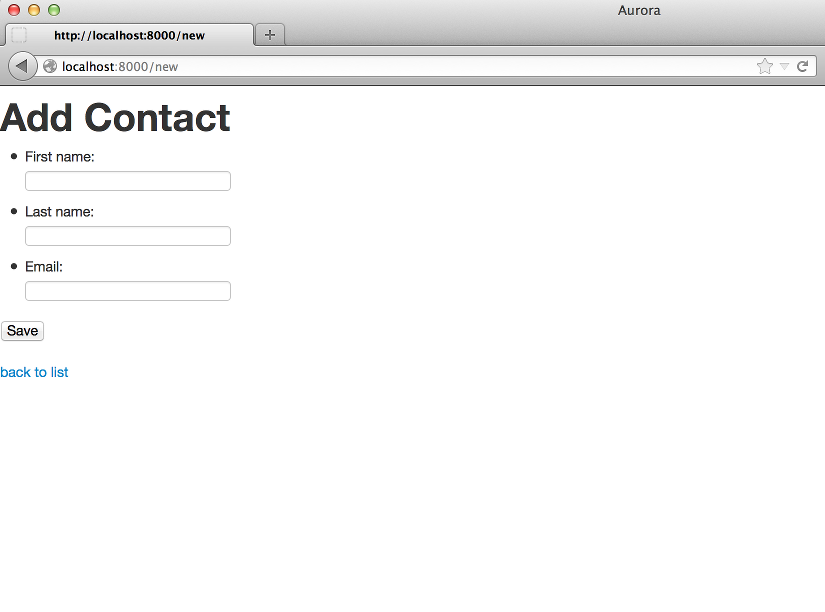
\includegraphics{boostrapped.png}


\section{Review}
\label{tutorial/static:review}\begin{itemize}
\item {} 
Django distinguishes between static site files, and user uploaded
media

\item {} 
The \code{staticfiles} app is included to help manage static files and
serve them during development

\item {} 
Static files can be included with apps, or with the project. Choose
where you put them based on whether you expect all users of your app
to need them.

\item {} 
Templates can extend one another, using \code{block} tags.

\end{itemize}


\chapter{Additional Generic Views}
\label{tutorial/additional-views:deploying-static-files}\label{tutorial/additional-views::doc}\label{tutorial/additional-views:additional-generic-views}

\section{Edit Views}
\label{tutorial/additional-views:edit-views}
In addition to creating Contacts, we'll of course want to edit them.
As with the List and Create views, Django has a generic view we can
use as a starting point.

\begin{Verbatim}[commandchars=\\\{\}]
\PYG{k+kn}{from} \PYG{n+nn}{django.views.generic} \PYG{k+kn}{import} \PYG{n}{UpdateView}
\PYG{o}{.}\PYG{o}{.}\PYG{o}{.}
\PYG{k}{class} \PYG{n+nc}{UpdateContactView}\PYG{p}{(}\PYG{n}{UpdateView}\PYG{p}{)}\PYG{p}{:}

    \PYG{n}{model} \PYG{o}{=} \PYG{n}{Contact}
    \PYG{n}{template\PYGZus{}name} \PYG{o}{=} \PYG{l+s}{\PYGZsq{}}\PYG{l+s}{edit\PYGZus{}contact.html}\PYG{l+s}{\PYGZsq{}}

    \PYG{k}{def} \PYG{n+nf}{get\PYGZus{}success\PYGZus{}url}\PYG{p}{(}\PYG{n+nb+bp}{self}\PYG{p}{)}\PYG{p}{:}
        \PYG{k}{return} \PYG{n}{reverse}\PYG{p}{(}\PYG{l+s}{\PYGZsq{}}\PYG{l+s}{contacts\PYGZhy{}list}\PYG{l+s}{\PYGZsq{}}\PYG{p}{)}
\end{Verbatim}
\begin{itemize}
\item {} 
we can re-use the same template

\item {} 
but how does it know which contact to load?

\item {} 
we need to either: provide a pk/slug, or override get\_object().

\item {} 
we'll provide pk in the URL

\end{itemize}

\begin{Verbatim}[commandchars=\\\{\}]
    \PYG{n}{url}\PYG{p}{(}\PYG{l+s}{r\PYGZsq{}}\PYG{l+s}{\PYGZca{}edit/(?P\PYGZlt{}pk\PYGZgt{}}\PYG{l+s}{\PYGZbs{}}\PYG{l+s}{d+)/\PYGZdl{}}\PYG{l+s}{\PYGZsq{}}\PYG{p}{,} \PYG{n}{contacts}\PYG{o}{.}\PYG{n}{views}\PYG{o}{.}\PYG{n}{UpdateContactView}\PYG{o}{.}\PYG{n}{as\PYGZus{}view}\PYG{p}{(}\PYG{p}{)}\PYG{p}{,}
        \PYG{n}{name}\PYG{o}{=}\PYG{l+s}{\PYGZsq{}}\PYG{l+s}{contacts\PYGZhy{}edit}\PYG{l+s}{\PYGZsq{}}\PYG{p}{,}\PYG{p}{)}\PYG{p}{,}
\end{Verbatim}

We'll update the contact list to include an edit link next to each
contact.

\begin{Verbatim}[commandchars=\\\{\}]
\PYGZob{}\PYGZpc{} extends \PYGZdq{}base.html\PYGZdq{} \PYGZpc{}\PYGZcb{}

\PYGZob{}\PYGZpc{} block content \PYGZpc{}\PYGZcb{}
\PYGZlt{}h1\PYGZgt{}Contacts\PYGZlt{}/h1\PYGZgt{}

\PYGZlt{}ul\PYGZgt{}
  \PYGZob{}\PYGZpc{} for contact in object\PYGZus{}list \PYGZpc{}\PYGZcb{}
    \PYGZlt{}li class=\PYGZdq{}contact\PYGZdq{}\PYGZgt{}\PYGZob{}\PYGZob{} contact \PYGZcb{}\PYGZcb{}
      (\PYGZlt{}a href=\PYGZdq{}\PYGZob{}\PYGZpc{} url \PYGZdq{}contacts\PYGZhy{}edit\PYGZdq{} pk=contact.id \PYGZpc{}\PYGZcb{}\PYGZdq{}\PYGZgt{}edit\PYGZlt{}/a\PYGZgt{})
    \PYGZlt{}/li\PYGZgt{}
  \PYGZob{}\PYGZpc{} endfor \PYGZpc{}\PYGZcb{}
\PYGZlt{}/ul\PYGZgt{}

\PYGZlt{}a href=\PYGZdq{}\PYGZob{}\PYGZpc{} url \PYGZdq{}contacts\PYGZhy{}new\PYGZdq{} \PYGZpc{}\PYGZcb{}\PYGZdq{}\PYGZgt{}add contact\PYGZlt{}/a\PYGZgt{}
\PYGZob{}\PYGZpc{} endblock \PYGZpc{}\PYGZcb{}
\end{Verbatim}

Note the use of \code{pk=contact.id} in the \code{\{\% url \%\}} tag to specify
the arguments to fill into the URL pattern.

If you run the server now, you'll see an edit link. Go ahead and click
it, and try to make a change. You'll notice that instead of editing
the existing record, it creates a new one. Sad face.

If we look at the source of the edit HTML, we can easily see the
reason: the form targets \code{/new}, not our edit URL. To fix this --
and still allow re-using the template -- we're going to add some
information to the template context.

The template context is the information available to a template when
it's rendered. This is a combination of information you provide in
your view -- either directly or indirectly -- and information added by
\href{https://docs.djangoproject.com/en/1.5/ref/templates/api/\#subclassing-context-requestcontext}{context processors} (https://docs.djangoproject.com/en/1.5/ref/templates/api/\#subclassing-context-requestcontext), such as the location for static media and
current locale. In order to use the same template for add and edit,
we'll add information about where the form should redirect to the
context.

\begin{Verbatim}[commandchars=\\\{\}]
\PYG{k}{class} \PYG{n+nc}{CreateContactView}\PYG{p}{(}\PYG{n}{CreateView}\PYG{p}{)}\PYG{p}{:}

    \PYG{n}{model} \PYG{o}{=} \PYG{n}{Contact}
    \PYG{n}{template\PYGZus{}name} \PYG{o}{=} \PYG{l+s}{\PYGZsq{}}\PYG{l+s}{edit\PYGZus{}contact.html}\PYG{l+s}{\PYGZsq{}}

    \PYG{k}{def} \PYG{n+nf}{get\PYGZus{}success\PYGZus{}url}\PYG{p}{(}\PYG{n+nb+bp}{self}\PYG{p}{)}\PYG{p}{:}
        \PYG{k}{return} \PYG{n}{reverse}\PYG{p}{(}\PYG{l+s}{\PYGZsq{}}\PYG{l+s}{contacts\PYGZhy{}list}\PYG{l+s}{\PYGZsq{}}\PYG{p}{)}

    \PYG{k}{def} \PYG{n+nf}{get\PYGZus{}context\PYGZus{}data}\PYG{p}{(}\PYG{n+nb+bp}{self}\PYG{p}{,} \PYG{o}{*}\PYG{o}{*}\PYG{n}{kwargs}\PYG{p}{)}\PYG{p}{:}

        \PYG{n}{context} \PYG{o}{=} \PYG{n+nb}{super}\PYG{p}{(}\PYG{n}{CreateContactView}\PYG{p}{,} \PYG{n+nb+bp}{self}\PYG{p}{)}\PYG{o}{.}\PYG{n}{get\PYGZus{}context\PYGZus{}data}\PYG{p}{(}\PYG{o}{*}\PYG{o}{*}\PYG{n}{kwargs}\PYG{p}{)}
        \PYG{n}{context}\PYG{p}{[}\PYG{l+s}{\PYGZsq{}}\PYG{l+s}{action}\PYG{l+s}{\PYGZsq{}}\PYG{p}{]} \PYG{o}{=} \PYG{n}{reverse}\PYG{p}{(}\PYG{l+s}{\PYGZsq{}}\PYG{l+s}{contacts\PYGZhy{}new}\PYG{l+s}{\PYGZsq{}}\PYG{p}{)}

        \PYG{k}{return} \PYG{n}{context}
\end{Verbatim}

\begin{Verbatim}[commandchars=\\\{\}]
\PYG{k}{class} \PYG{n+nc}{UpdateContactView}\PYG{p}{(}\PYG{n}{UpdateView}\PYG{p}{)}\PYG{p}{:}

    \PYG{n}{model} \PYG{o}{=} \PYG{n}{Contact}
    \PYG{n}{template\PYGZus{}name} \PYG{o}{=} \PYG{l+s}{\PYGZsq{}}\PYG{l+s}{edit\PYGZus{}contact.html}\PYG{l+s}{\PYGZsq{}}

    \PYG{k}{def} \PYG{n+nf}{get\PYGZus{}success\PYGZus{}url}\PYG{p}{(}\PYG{n+nb+bp}{self}\PYG{p}{)}\PYG{p}{:}
        \PYG{k}{return} \PYG{n}{reverse}\PYG{p}{(}\PYG{l+s}{\PYGZsq{}}\PYG{l+s}{contacts\PYGZhy{}list}\PYG{l+s}{\PYGZsq{}}\PYG{p}{)}

    \PYG{k}{def} \PYG{n+nf}{get\PYGZus{}context\PYGZus{}data}\PYG{p}{(}\PYG{n+nb+bp}{self}\PYG{p}{,} \PYG{o}{*}\PYG{o}{*}\PYG{n}{kwargs}\PYG{p}{)}\PYG{p}{:}

        \PYG{n}{context} \PYG{o}{=} \PYG{n+nb}{super}\PYG{p}{(}\PYG{n}{UpdateContactView}\PYG{p}{,} \PYG{n+nb+bp}{self}\PYG{p}{)}\PYG{o}{.}\PYG{n}{get\PYGZus{}context\PYGZus{}data}\PYG{p}{(}\PYG{o}{*}\PYG{o}{*}\PYG{n}{kwargs}\PYG{p}{)}
        \PYG{n}{context}\PYG{p}{[}\PYG{l+s}{\PYGZsq{}}\PYG{l+s}{action}\PYG{l+s}{\PYGZsq{}}\PYG{p}{]} \PYG{o}{=} \PYG{n}{reverse}\PYG{p}{(}\PYG{l+s}{\PYGZsq{}}\PYG{l+s}{contacts\PYGZhy{}edit}\PYG{l+s}{\PYGZsq{}}\PYG{p}{,}
                                    \PYG{n}{kwargs}\PYG{o}{=}\PYG{p}{\PYGZob{}}\PYG{l+s}{\PYGZsq{}}\PYG{l+s}{pk}\PYG{l+s}{\PYGZsq{}}\PYG{p}{:} \PYG{n+nb+bp}{self}\PYG{o}{.}\PYG{n}{get\PYGZus{}object}\PYG{p}{(}\PYG{p}{)}\PYG{o}{.}\PYG{n}{id}\PYG{p}{\PYGZcb{}}\PYG{p}{)}

        \PYG{k}{return} \PYG{n}{context}
\end{Verbatim}

We also update the template to use that value for the action and
change the title based on whether or not we've previously saved.

\begin{Verbatim}[commandchars=\\\{\}]
\PYGZob{}\PYGZpc{} if contact.id \PYGZpc{}\PYGZcb{}
\PYG{n+nt}{\PYGZlt{}h1}\PYG{n+nt}{\PYGZgt{}}Edit Contact\PYG{n+nt}{\PYGZlt{}/h1\PYGZgt{}}
\PYGZob{}\PYGZpc{} else \PYGZpc{}\PYGZcb{}
\PYG{n+nt}{\PYGZlt{}h1}\PYG{n+nt}{\PYGZgt{}}Add Contact\PYG{n+nt}{\PYGZlt{}/h1\PYGZgt{}}
\PYGZob{}\PYGZpc{} endif \PYGZpc{}\PYGZcb{}

\PYG{n+nt}{\PYGZlt{}form} \PYG{n+na}{action=}\PYG{l+s}{\PYGZdq{}\PYGZob{}\PYGZob{} action \PYGZcb{}\PYGZcb{}\PYGZdq{}} \PYG{n+na}{method=}\PYG{l+s}{\PYGZdq{}POST\PYGZdq{}}\PYG{n+nt}{\PYGZgt{}}
\end{Verbatim}

You may wonder where the \code{contact} value in the contact comes from:
the class based views that wrap a single object (those that take
a primary key or slug) expose that to the context in two different
ways: as a variable named \code{object}, and as a variable named after
the model class. The latter often makes your templates easier to read
and understand later. You can customize this name by overriding
\code{get\_context\_object\_name} on your view.
\setbox0\vbox{
\begin{minipage}{0.95\linewidth}
\textbf{Made a Change? Run the Tests.}

\medskip


We've just made a change to our \code{CreateContactView}, which means
this is a perfect time to run the tests we wrote. Do they still pass?
If not, did we introduce a bug, or did the behavior change in a way
that we expected?

(Hint: We changed how the contact list is rendered, so our tests
that just expect the name there are going to fail. This is a case
where you'd need to update the test case, but it also demonstrates
how integration tests can be fragile.)
\end{minipage}}
\begin{center}\setlength{\fboxsep}{5pt}\shadowbox{\box0}\end{center}


\section{Deleting Contacts}
\label{tutorial/additional-views:deleting-contacts}
The final view for our basic set of views is delete. The generic
deletion view is very similar to the edit view: it wraps a single
object and requires that you provide a URL to redirect to on success.
When it processes a HTTP GET request, it displays a confirmation page,
and when it receives an HTTP DELETE or POST, it deletes the object and
redirects to the success URL.

We add the view definition to \code{views.py}:

\begin{Verbatim}[commandchars=\\\{\}]
\PYG{k+kn}{from} \PYG{n+nn}{django.views.generic} \PYG{k+kn}{import} \PYG{n}{DeleteView}
\PYG{o}{.}\PYG{o}{.}\PYG{o}{.}
\PYG{k}{class} \PYG{n+nc}{DeleteContactView}\PYG{p}{(}\PYG{n}{DeleteView}\PYG{p}{)}\PYG{p}{:}

    \PYG{n}{model} \PYG{o}{=} \PYG{n}{Contact}
    \PYG{n}{template\PYGZus{}name} \PYG{o}{=} \PYG{l+s}{\PYGZsq{}}\PYG{l+s}{delete\PYGZus{}contact.html}\PYG{l+s}{\PYGZsq{}}

    \PYG{k}{def} \PYG{n+nf}{get\PYGZus{}success\PYGZus{}url}\PYG{p}{(}\PYG{n+nb+bp}{self}\PYG{p}{)}\PYG{p}{:}
        \PYG{k}{return} \PYG{n}{reverse}\PYG{p}{(}\PYG{l+s}{\PYGZsq{}}\PYG{l+s}{contacts\PYGZhy{}list}\PYG{l+s}{\PYGZsq{}}\PYG{p}{)}
\end{Verbatim}

And create the template, \code{delete\_contact.html}, in our \code{templates}
directory.

\begin{Verbatim}[commandchars=\\\{\}]
\PYGZob{}\PYGZpc{} extends \PYGZdq{}base.html\PYGZdq{} \PYGZpc{}\PYGZcb{}

\PYGZob{}\PYGZpc{} block content \PYGZpc{}\PYGZcb{}

\PYGZlt{}h1\PYGZgt{}Delete Contact\PYGZlt{}/h1\PYGZgt{}

\PYGZlt{}p\PYGZgt{}Are you sure you want to delete the contact \PYGZob{}\PYGZob{} contact \PYGZcb{}\PYGZcb{}?\PYGZlt{}/p\PYGZgt{}

\PYGZlt{}form action=\PYGZdq{}\PYGZob{}\PYGZpc{} url \PYGZdq{}contacts\PYGZhy{}delete\PYGZdq{} pk=contact.id \PYGZpc{}\PYGZcb{}\PYGZdq{} method=\PYGZdq{}POST\PYGZdq{}\PYGZgt{}
  \PYGZob{}\PYGZpc{} csrf\PYGZus{}token \PYGZpc{}\PYGZcb{}

  \PYGZlt{}input type=\PYGZdq{}submit\PYGZdq{} value=\PYGZdq{}Yes, delete.\PYGZdq{} /\PYGZgt{}
  \PYGZlt{}a href=\PYGZdq{}\PYGZob{}\PYGZpc{} url \PYGZdq{}contacts\PYGZhy{}list\PYGZdq{} \PYGZpc{}\PYGZcb{}\PYGZdq{}\PYGZgt{}No, cancel.\PYGZlt{}/a\PYGZgt{}
\PYGZlt{}/form\PYGZgt{}

\PYGZob{}\PYGZpc{} endblock \PYGZpc{}\PYGZcb{}
\end{Verbatim}

Of course we need to add this to the URL definitions:

\begin{Verbatim}[commandchars=\\\{\}]
    \PYG{n}{url}\PYG{p}{(}\PYG{l+s}{r\PYGZsq{}}\PYG{l+s}{\PYGZca{}delete/(?P\PYGZlt{}pk\PYGZgt{}}\PYG{l+s}{\PYGZbs{}}\PYG{l+s}{d+)/\PYGZdl{}}\PYG{l+s}{\PYGZsq{}}\PYG{p}{,} \PYG{n}{contacts}\PYG{o}{.}\PYG{n}{views}\PYG{o}{.}\PYG{n}{DeleteContactView}\PYG{o}{.}\PYG{n}{as\PYGZus{}view}\PYG{p}{(}\PYG{p}{)}\PYG{p}{,}
        \PYG{n}{name}\PYG{o}{=}\PYG{l+s}{\PYGZsq{}}\PYG{l+s}{contacts\PYGZhy{}delete}\PYG{l+s}{\PYGZsq{}}\PYG{p}{,}\PYG{p}{)}\PYG{p}{,}
\end{Verbatim}

And we'll add the link to delete to the edit page.

\begin{Verbatim}[commandchars=\\\{\}]
\PYGZob{}\PYGZpc{} if contact.id \PYGZpc{}\PYGZcb{}
\PYGZlt{}a href=\PYGZdq{}\PYGZob{}\PYGZpc{} url \PYGZdq{}contacts\PYGZhy{}delete\PYGZdq{} pk=contact.id \PYGZpc{}\PYGZcb{}\PYGZdq{}\PYGZgt{}Delete\PYGZlt{}/a\PYGZgt{}
\PYGZob{}\PYGZpc{} endif \PYGZpc{}\PYGZcb{}
\end{Verbatim}


\section{Detail View}
\label{tutorial/additional-views:detail-view}
Finally, let's go ahead and add a detail view for our Contacts. This
will show the details of the Contact: not much right now, but we'll
build on this shortly. Django includes a generic \code{DetailView}: think
of it as the single serving \code{ListView}.

\begin{Verbatim}[commandchars=\\\{\}]
\PYG{k+kn}{from} \PYG{n+nn}{django.views.generic} \PYG{k+kn}{import} \PYG{n}{DetailView}
\PYG{o}{.}\PYG{o}{.}\PYG{o}{.}
\PYG{k}{class} \PYG{n+nc}{ContactView}\PYG{p}{(}\PYG{n}{DetailView}\PYG{p}{)}\PYG{p}{:}

    \PYG{n}{model} \PYG{o}{=} \PYG{n}{Contact}
    \PYG{n}{template\PYGZus{}name} \PYG{o}{=} \PYG{l+s}{\PYGZsq{}}\PYG{l+s}{contact.html}\PYG{l+s}{\PYGZsq{}}
\end{Verbatim}

Again, the template is pretty straight forward; we create
\code{contact.html} in the \code{templates} directory.

\begin{Verbatim}[commandchars=\\\{\}]
\PYGZob{}\PYGZpc{} extends \PYGZdq{}base.html\PYGZdq{} \PYGZpc{}\PYGZcb{}

\PYGZob{}\PYGZpc{} block content \PYGZpc{}\PYGZcb{}

\PYG{n+nt}{\PYGZlt{}h1}\PYG{n+nt}{\PYGZgt{}}\PYGZob{}\PYGZob{} contact \PYGZcb{}\PYGZcb{}\PYG{n+nt}{\PYGZlt{}/h1\PYGZgt{}}

\PYG{n+nt}{\PYGZlt{}p}\PYG{n+nt}{\PYGZgt{}}Email: \PYGZob{}\PYGZob{} contact.email \PYGZcb{}\PYGZcb{}\PYG{n+nt}{\PYGZlt{}/p\PYGZgt{}}

\PYGZob{}\PYGZpc{} endblock \PYGZpc{}\PYGZcb{}
\end{Verbatim}

And add the URL mapping:

\begin{Verbatim}[commandchars=\\\{\}]
    \PYG{n}{url}\PYG{p}{(}\PYG{l+s}{r\PYGZsq{}}\PYG{l+s}{\PYGZca{}(?P\PYGZlt{}pk\PYGZgt{}}\PYG{l+s}{\PYGZbs{}}\PYG{l+s}{d+)/\PYGZdl{}}\PYG{l+s}{\PYGZsq{}}\PYG{p}{,} \PYG{n}{contacts}\PYG{o}{.}\PYG{n}{views}\PYG{o}{.}\PYG{n}{ContactView}\PYG{o}{.}\PYG{n}{as\PYGZus{}view}\PYG{p}{(}\PYG{p}{)}\PYG{p}{,}
        \PYG{n}{name}\PYG{o}{=}\PYG{l+s}{\PYGZsq{}}\PYG{l+s}{contacts\PYGZhy{}view}\PYG{l+s}{\PYGZsq{}}\PYG{p}{,}\PYG{p}{)}\PYG{p}{,}
\end{Verbatim}

We're also going to add a method to our Contact model,
\code{get\_absolute\_url}. \code{get\_absolute\_url} is a Django convention for
obtaining the URL of a single model instance. In this case it's just
going to be a call to \code{reverse}, but by providing this method, our
model will play nicely with other parts of Django.

\begin{Verbatim}[commandchars=\\\{\}]
class Contact(models.Model):
...
    def get\PYGZus{}absolute\PYGZus{}url(self):

        return reverse(\PYGZsq{}contacts\PYGZhy{}view\PYGZsq{}, kwargs=\PYGZob{}\PYGZsq{}pk\PYGZsq{}: self.id\PYGZcb{})
\end{Verbatim}

And we'll add the link to the contact from the contact list.

\begin{Verbatim}[commandchars=\\\{\}]
  \PYGZob{}\PYGZpc{} for contact in object\PYGZus{}list \PYGZpc{}\PYGZcb{}
    \PYGZlt{}li class=\PYGZdq{}contact\PYGZdq{}\PYGZgt{}
      \PYGZlt{}a href=\PYGZdq{}\PYGZob{}\PYGZob{} contact.get\PYGZus{}absolute\PYGZus{}url \PYGZcb{}\PYGZcb{}\PYGZdq{}\PYGZgt{}\PYGZob{}\PYGZob{} contact \PYGZcb{}\PYGZcb{}\PYGZlt{}/a\PYGZgt{}
      (\PYGZlt{}a href=\PYGZdq{}\PYGZob{}\PYGZpc{} url \PYGZdq{}contacts\PYGZhy{}edit\PYGZdq{} pk=contact.id \PYGZpc{}\PYGZcb{}\PYGZdq{}\PYGZgt{}edit\PYGZlt{}/a\PYGZgt{})
    \PYGZlt{}/li\PYGZgt{}
  \PYGZob{}\PYGZpc{} endfor \PYGZpc{}\PYGZcb{}
\end{Verbatim}


\chapter{Form Basics}
\label{tutorial/forms::doc}\label{tutorial/forms:selenium}\label{tutorial/forms:form-basics}\DUspan{admonition-django-forms}{}\DUspan{admonition-defining-forms}{}\DUspan{admonition-instantiating-a-form}{}\DUspan{admonition-accessing-fields}{}\DUspan{admonition-validating-the-form}{}\DUspan{admonition-field-validation}{}\DUspan{admonition-field-cleaning}{}
Up until this point we've been using forms without really needing to
be aware of it. A \href{https://docs.djangoproject.com/en/1.5/topics/forms/}{Django Form} (https://docs.djangoproject.com/en/1.5/topics/forms/) is responsible for taking some user
input, validating it, and turning it into Python objects. They also
have some handy rendering methods, but I consider those sugar: the
real power is in making sure that input from your users is what it
says it is.

The \href{https://docs.djangoproject.com/en/1.5/topics/class-based-views/}{Generic Views} (https://docs.djangoproject.com/en/1.5/topics/class-based-views/), specifically the ones we've been using, all
operate on a particular model. Django is able to take the model
definition that we've created and extrapolate a Form from it. Django
can do this because both Models and Forms are constructed of fields
that have a particular type and particular validation rules. Models
use those fields to map data to types that your database understands;
Forms use them to map input to Python types \footnote{
While I'm referring to them both as fields, they're really
completely different implementations. But the analogy holds.
}. Forms that map to a
particular Model are called \href{https://docs.djangoproject.com/en/1.5/topics/forms/modelforms}{ModelForms} (https://docs.djangoproject.com/en/1.5/topics/forms/modelforms); you can think of them as
taking user input and transforming it into an instance of a Model.


\section{Adding Fields to the Form}
\label{tutorial/forms:adding-fields-to-the-form}
So what if we want to add a field to our form? Say, we want to require
confirmation of the email address. In that case we can create a new
form, and override the default used by our views.

First, in the \code{contacts} app directory, we'll create a new file,
\code{forms.py}.

\begin{Verbatim}[commandchars=\\\{\}]
\PYG{k+kn}{from} \PYG{n+nn}{django} \PYG{k+kn}{import} \PYG{n}{forms}
\PYG{k+kn}{from} \PYG{n+nn}{django.core.exceptions} \PYG{k+kn}{import} \PYG{n}{ValidationError}

\PYG{k+kn}{from} \PYG{n+nn}{contacts.models} \PYG{k+kn}{import} \PYG{n}{Contact}


\PYG{k}{class} \PYG{n+nc}{ContactForm}\PYG{p}{(}\PYG{n}{forms}\PYG{o}{.}\PYG{n}{ModelForm}\PYG{p}{)}\PYG{p}{:}

    \PYG{n}{confirm\PYGZus{}email} \PYG{o}{=} \PYG{n}{forms}\PYG{o}{.}\PYG{n}{EmailField}\PYG{p}{(}
        \PYG{n}{label}\PYG{o}{=}\PYG{l+s}{\PYGZdq{}}\PYG{l+s}{Confirm email}\PYG{l+s}{\PYGZdq{}}\PYG{p}{,}
        \PYG{n}{required}\PYG{o}{=}\PYG{n+nb+bp}{True}\PYG{p}{,}
    \PYG{p}{)}

    \PYG{k}{class} \PYG{n+nc}{Meta}\PYG{p}{:}
        \PYG{n}{model} \PYG{o}{=} \PYG{n}{Contact}

    \PYG{k}{def} \PYG{n+nf}{\PYGZus{}\PYGZus{}init\PYGZus{}\PYGZus{}}\PYG{p}{(}\PYG{n+nb+bp}{self}\PYG{p}{,} \PYG{o}{*}\PYG{n}{args}\PYG{p}{,} \PYG{o}{*}\PYG{o}{*}\PYG{n}{kwargs}\PYG{p}{)}\PYG{p}{:}

        \PYG{k}{if} \PYG{n}{kwargs}\PYG{o}{.}\PYG{n}{get}\PYG{p}{(}\PYG{l+s}{\PYGZsq{}}\PYG{l+s}{instance}\PYG{l+s}{\PYGZsq{}}\PYG{p}{)}\PYG{p}{:}
            \PYG{n}{email} \PYG{o}{=} \PYG{n}{kwargs}\PYG{p}{[}\PYG{l+s}{\PYGZsq{}}\PYG{l+s}{instance}\PYG{l+s}{\PYGZsq{}}\PYG{p}{]}\PYG{o}{.}\PYG{n}{email}
            \PYG{n}{kwargs}\PYG{o}{.}\PYG{n}{setdefault}\PYG{p}{(}\PYG{l+s}{\PYGZsq{}}\PYG{l+s}{initial}\PYG{l+s}{\PYGZsq{}}\PYG{p}{,} \PYG{p}{\PYGZob{}}\PYG{p}{\PYGZcb{}}\PYG{p}{)}\PYG{p}{[}\PYG{l+s}{\PYGZsq{}}\PYG{l+s}{confirm\PYGZus{}email}\PYG{l+s}{\PYGZsq{}}\PYG{p}{]} \PYG{o}{=} \PYG{n}{email}

        \PYG{k}{return} \PYG{n+nb}{super}\PYG{p}{(}\PYG{n}{ContactForm}\PYG{p}{,} \PYG{n+nb+bp}{self}\PYG{p}{)}\PYG{o}{.}\PYG{n}{\PYGZus{}\PYGZus{}init\PYGZus{}\PYGZus{}}\PYG{p}{(}\PYG{o}{*}\PYG{n}{args}\PYG{p}{,} \PYG{o}{*}\PYG{o}{*}\PYG{n}{kwargs}\PYG{p}{)}
\end{Verbatim}

Here we're creating a new \code{ModelForm}; we associate the form with
our model in the \code{Meta} inner class.

We're also adding an additional field, \code{confirm\_email}. This is an
example of a field declaration in a model. The first argument is the
label, and then there are additional keyword arguments; in this case,
we simply mark it required.

Finally, in the constructor we mutate the \code{initial} kwarg.
\code{initial} is a dictionary of values that will be used as the default
values for an \href{https://docs.djangoproject.com/en/1.5/ref/forms/api/\#ref-forms-api-bound-unbound}{unbound form} (https://docs.djangoproject.com/en/1.5/ref/forms/api/\#ref-forms-api-bound-unbound). Model Forms have another kwarg,
\code{instance}, that holds the instance we're editing.


\section{Overriding the Default Form}
\label{tutorial/forms:overriding-the-default-form}
We've defined a form with the extra field, but we still need to tell
our view to use it. You can do this in a couple of ways, but the
simplest is to set the \code{form\_class} property on the View class.
We'll add that property to our \code{CreateContactView} and
\code{UpdateContactView} in \code{views.py}.

\begin{Verbatim}[commandchars=\\\{\}]
\PYG{k+kn}{import} \PYG{n+nn}{forms}
\PYG{o}{.}\PYG{o}{.}\PYG{o}{.}
\PYG{k}{class} \PYG{n+nc}{CreateContactView}\PYG{p}{(}\PYG{n}{CreateView}\PYG{p}{)}\PYG{p}{:}

    \PYG{n}{model} \PYG{o}{=} \PYG{n}{Contact}
    \PYG{n}{template\PYGZus{}name} \PYG{o}{=} \PYG{l+s}{\PYGZsq{}}\PYG{l+s}{edit\PYGZus{}contact.html}\PYG{l+s}{\PYGZsq{}}
    \PYG{n}{form\PYGZus{}class} \PYG{o}{=} \PYG{n}{forms}\PYG{o}{.}\PYG{n}{ContactForm}
\end{Verbatim}

\begin{Verbatim}[commandchars=\\\{\}]
\PYG{k}{class} \PYG{n+nc}{UpdateContactView}\PYG{p}{(}\PYG{n}{UpdateView}\PYG{p}{)}\PYG{p}{:}

    \PYG{n}{model} \PYG{o}{=} \PYG{n}{Contact}
    \PYG{n}{template\PYGZus{}name} \PYG{o}{=} \PYG{l+s}{\PYGZsq{}}\PYG{l+s}{edit\PYGZus{}contact.html}\PYG{l+s}{\PYGZsq{}}
    \PYG{n}{form\PYGZus{}class} \PYG{o}{=} \PYG{n}{forms}\PYG{o}{.}\PYG{n}{ContactForm}
\end{Verbatim}

If we fire up the server and visit the edit or create pages, we'll see
the additional field. We can see that it's required, but there's no
validation that the two fields match. To support that we'll need to
add some custom validation to the Form.


\section{Customizing Validation}
\label{tutorial/forms:customizing-validation}
Forms have two different phases of validation: field and form. All the
fields are validated and converted to Python objects (if possible)
before form validation begins.

Field validation takes place for an individual field: things like
minimum and maximum length, making sure it looks like a URL, and date
range validation are all examples of field validation. Django doesn't
guarantee that field validation happens in any order, so you can't
count on other fields being available for comparison during this
phase.

Form validation, on the other hand, happens after all fields have been
validated and converted to Python objects, and gives you the
opportunity to do things like make sure passwords match, or in this
case, email addresses.

Form validation takes place in a form's \code{clean()} method.

\begin{Verbatim}[commandchars=\\\{\}]
\PYG{k}{class} \PYG{n+nc}{ContactForm}\PYG{p}{(}\PYG{n}{forms}\PYG{o}{.}\PYG{n}{ModelForm}\PYG{p}{)}\PYG{p}{:}
\PYG{o}{.}\PYG{o}{.}\PYG{o}{.}
    \PYG{k}{def} \PYG{n+nf}{clean}\PYG{p}{(}\PYG{n+nb+bp}{self}\PYG{p}{)}\PYG{p}{:}

        \PYG{k}{if} \PYG{p}{(}\PYG{n+nb+bp}{self}\PYG{o}{.}\PYG{n}{cleaned\PYGZus{}data}\PYG{o}{.}\PYG{n}{get}\PYG{p}{(}\PYG{l+s}{\PYGZsq{}}\PYG{l+s}{email}\PYG{l+s}{\PYGZsq{}}\PYG{p}{)} \PYG{o}{!=}
            \PYG{n+nb+bp}{self}\PYG{o}{.}\PYG{n}{cleaned\PYGZus{}data}\PYG{o}{.}\PYG{n}{get}\PYG{p}{(}\PYG{l+s}{\PYGZsq{}}\PYG{l+s}{confirm\PYGZus{}email}\PYG{l+s}{\PYGZsq{}}\PYG{p}{)}\PYG{p}{)}\PYG{p}{:}

            \PYG{k}{raise} \PYG{n}{ValidationError}\PYG{p}{(}
                \PYG{l+s}{\PYGZdq{}}\PYG{l+s}{Email addresses must match.}\PYG{l+s}{\PYGZdq{}}
            \PYG{p}{)}

        \PYG{k}{return} \PYG{n+nb+bp}{self}\PYG{o}{.}\PYG{n}{cleaned\PYGZus{}data}
\end{Verbatim}

When you enter the \code{clean} method, all of the fields that validated
are available in the \code{cleaned\_data} dictionary. The \code{clean} method
may add, remove, or modify values, but \textbf{must} return the dictionary
of cleaned data. \code{clean} may also raise a \code{ValidationError} if it
encounters an error. This will be available as part of the forms'
\code{errors} property, and is shown by default when you render the form.

Note that I said \code{cleaned\_data} contains all the fields \emph{that
validated}. That's because form-level validation \textbf{always} happens,
even if no fields were successfully validated. That's why in the clean
method we use \code{cleaned\_data.get('email')} instead of
\code{cleaned\_data{[}'email'{]}}.

If you visit the create or update views now, we'll see an extra field
there. Try to make a change, or create a contact, without entering the
email address twice.


\section{Controlling Form Rendering}
\label{tutorial/forms:controlling-form-rendering}\DUspan{admonition-rendering-forms}{}
Our templates until now look pretty magical when it comes to forms:
the extent of our HTML tags has been something like:

\begin{Verbatim}[commandchars=\\\{\}]
\PYGZlt{}form action=\PYGZdq{}\PYGZob{}\PYGZob{} action \PYGZcb{}\PYGZcb{}\PYGZdq{} method=\PYGZdq{}POST\PYGZdq{}\PYGZgt{}
  \PYGZob{}\PYGZpc{} csrf\PYGZus{}token \PYGZpc{}\PYGZcb{}
  \PYGZlt{}ul\PYGZgt{}
    \PYGZob{}\PYGZob{} form.as\PYGZus{}ul \PYGZcb{}\PYGZcb{}
  \PYGZlt{}/ul\PYGZgt{}
  \PYGZlt{}input type=\PYGZdq{}submit\PYGZdq{} value=\PYGZdq{}Save\PYGZdq{} /\PYGZgt{}
\PYGZlt{}/form\PYGZgt{}
\end{Verbatim}

We're living at the whim of \code{form.as\_ul}, and it's likely we want
something different.

Forms have three pre-baked output formats: \code{as\_ul}, \code{as\_p}, and
\code{as\_table}. If \code{as\_ul} outputs the form elements as the items in
an unordered list, it's not too mysterious what \code{as\_p} and
\code{as\_table} do.
\DUspan{admonition-controlling-form-output}{}
Often, though, you need more control. For those cases, you can take
full control. First, a form is iterable; try replacing your call to
\code{\{\{form.as\_ul\}\}} with this:

\begin{Verbatim}[commandchars=\\\{\}]
\PYGZob{}\PYGZpc{} for field in form \PYGZpc{}\PYGZcb{}
\PYGZob{}\PYGZob{} field \PYGZcb{}\PYGZcb{}
\PYGZob{}\PYGZpc{} endfor \PYGZpc{}\PYGZcb{}
\end{Verbatim}

As you can see, \code{field} renders as the input for each field in the
form. When you iterate over a Form, you're iterating over a sequence
of \href{https://docs.djangoproject.com/en/1.5/ref/forms/api/\#django.forms.BoundField}{BoundField} (https://docs.djangoproject.com/en/1.5/ref/forms/api/\#django.forms.BoundField) objects. A \code{BoundField} wraps the field definition
from your Form (or derived from the ModelForm) along with any data and
error state it may be bound to. This means it has some properties that
are handy for customizing rendering.

In addition to supporting iteration, you can access an individual
BoundField directly, treating the Form like a dictionary:

\begin{Verbatim}[commandchars=\\\{\}]
\PYG{p}{\PYGZob{}}\PYG{p}{\PYGZob{}} \PYG{n}{form}\PYG{o}{.}\PYG{n}{email} \PYG{p}{\PYGZcb{}}\PYG{p}{\PYGZcb{}}
\end{Verbatim}
\setbox0\vbox{
\begin{minipage}{0.95\linewidth}
\textbf{Dictionary!?!}

\medskip


That may not look like a dictionary access, but remember that Django
templates are quite restrictive in their syntax. Writing \code{foo.bar}
will look for a property \code{bar} on \code{foo}, and if it's callable,
call it. If it doesn't find a property, it'll map that to something
like \code{foo{[}'bar'{]}}. So when it comes to writing Django templates,
dictionary elements act just like properties.
\end{minipage}}
\begin{center}\setlength{\fboxsep}{5pt}\shadowbox{\box0}\end{center}

Consider the following alternative to \code{edit\_contact.html}.

\begin{Verbatim}[commandchars=\\\{\}]
\PYGZob{}\PYGZpc{} extends \PYGZdq{}base.html\PYGZdq{} \PYGZpc{}\PYGZcb{}

\PYGZob{}\PYGZpc{} block content \PYGZpc{}\PYGZcb{}

\PYGZob{}\PYGZpc{} if contact.id \PYGZpc{}\PYGZcb{}
\PYGZlt{}h1\PYGZgt{}Edit Contact\PYGZlt{}/h1\PYGZgt{}
\PYGZob{}\PYGZpc{} else \PYGZpc{}\PYGZcb{}
\PYGZlt{}h1\PYGZgt{}Add Contact\PYGZlt{}/h1\PYGZgt{}
\PYGZob{}\PYGZpc{} endif \PYGZpc{}\PYGZcb{}

\PYGZlt{}form action=\PYGZdq{}\PYGZob{}\PYGZob{} action \PYGZcb{}\PYGZcb{}\PYGZdq{} method=\PYGZdq{}POST\PYGZdq{}\PYGZgt{}
  \PYGZob{}\PYGZpc{} csrf\PYGZus{}token \PYGZpc{}\PYGZcb{}
  \PYGZob{}\PYGZpc{} if form.non\PYGZus{}field\PYGZus{}errors \PYGZpc{}\PYGZcb{}
    \PYGZlt{}ul\PYGZgt{}
      \PYGZob{}\PYGZpc{} for error in form.non\PYGZus{}field\PYGZus{}errors \PYGZpc{}\PYGZcb{}
        \PYGZlt{}li\PYGZgt{}\PYGZob{}\PYGZob{} error \PYGZcb{}\PYGZcb{}\PYGZlt{}/li\PYGZgt{}
      \PYGZob{}\PYGZpc{} endfor \PYGZpc{}\PYGZcb{}
    \PYGZlt{}/ul\PYGZgt{}
  \PYGZob{}\PYGZpc{} endif \PYGZpc{}\PYGZcb{}
  \PYGZob{}\PYGZpc{} for field in form \PYGZpc{}\PYGZcb{}
  \PYGZlt{}div id=\PYGZdq{}\PYGZob{}\PYGZob{} field.auto\PYGZus{}id \PYGZcb{}\PYGZcb{}\PYGZus{}container\PYGZdq{}\PYGZgt{}
    \PYGZob{}\PYGZob{} field.help\PYGZus{}text \PYGZcb{}\PYGZcb{}
    \PYGZlt{}div\PYGZgt{}
      \PYGZob{}\PYGZob{} field.label\PYGZus{}tag \PYGZcb{}\PYGZcb{} \PYGZob{}\PYGZob{} field \PYGZcb{}\PYGZcb{}
    \PYGZlt{}/div\PYGZgt{}
    \PYGZlt{}div id=\PYGZdq{}\PYGZob{}\PYGZob{} field.auto\PYGZus{}id \PYGZcb{}\PYGZcb{}\PYGZus{}errors\PYGZdq{}\PYGZgt{}
      \PYGZob{}\PYGZob{} field.errors \PYGZcb{}\PYGZcb{}
    \PYGZlt{}/div\PYGZgt{}
  \PYGZlt{}/div\PYGZgt{}
  \PYGZob{}\PYGZpc{} endfor \PYGZpc{}\PYGZcb{}

  \PYGZlt{}input id=\PYGZdq{}save\PYGZus{}contact\PYGZdq{} type=\PYGZdq{}submit\PYGZdq{} value=\PYGZdq{}Save\PYGZdq{} /\PYGZgt{}
\PYGZlt{}/form\PYGZgt{}

\PYGZob{}\PYGZpc{} if contact.id \PYGZpc{}\PYGZcb{}
\PYGZlt{}a href=\PYGZdq{}\PYGZob{}\PYGZpc{} url \PYGZdq{}contacts\PYGZhy{}edit\PYGZhy{}addresses\PYGZdq{} pk=contact.id \PYGZpc{}\PYGZcb{}\PYGZdq{}\PYGZgt{}
  Edit Addresses
\PYGZlt{}/a\PYGZgt{}
\PYGZlt{}a href=\PYGZdq{}\PYGZob{}\PYGZpc{} url \PYGZdq{}contacts\PYGZhy{}delete\PYGZdq{} pk=contact.id \PYGZpc{}\PYGZcb{}\PYGZdq{}\PYGZgt{}Delete\PYGZlt{}/a\PYGZgt{}
\PYGZob{}\PYGZpc{} endif \PYGZpc{}\PYGZcb{}

\PYGZlt{}a href=\PYGZdq{}\PYGZob{}\PYGZpc{} url \PYGZdq{}contacts\PYGZhy{}list\PYGZdq{} \PYGZpc{}\PYGZcb{}\PYGZdq{}\PYGZgt{}back to list\PYGZlt{}/a\PYGZgt{}

\PYGZob{}\PYGZpc{} endblock \PYGZpc{}\PYGZcb{}
\end{Verbatim}

In this example we see a few different things at work:
\begin{itemize}
\item {} 
\code{field.auto\_id} to get the automatically generated field ID

\item {} 
Combining that ID with \code{\_container} and \code{\_errors} to give our
related elements names that consistently match

\item {} 
Using \code{field.label\_tag} to generate the label. \code{label\_tag} adds
the appropriate \code{for} property to the tag, too. For the
\code{last\_name} field, this looks like:

\begin{Verbatim}[commandchars=\\\{\}]
\PYGZlt{}label for=\PYGZdq{}id\PYGZus{}last\PYGZus{}name\PYGZdq{}\PYGZgt{}Last name\PYGZlt{}/label\PYGZgt{}
\end{Verbatim}

\item {} 
Using \code{field.errors} to show the errors in a specific place. The
Django Form documentation has details on further customizing \href{https://docs.djangoproject.com/en/1.5/ref/forms/api/\#how-errors-are-displayed}{how
errors are displayed} (https://docs.djangoproject.com/en/1.5/ref/forms/api/\#how-errors-are-displayed).

\item {} 
Finally, \code{field.help\_text}. You can specify a \code{help\_text}
keyword argument to each field when creating your form, which is
accessible here. Defining that text in the Form definition is
desirable because you can easily mark it up for translation.

\end{itemize}


\section{Testing Forms}
\label{tutorial/forms:testing-forms}
It's easy to imagine how you'd use the \code{LiveServerTestCase} to write
an integration test for a Form. But that wouldn't just be testing the
Form, that'd be testing the View, the URL configuration, and probably
the Model (in this case, at least). We've built some custom logic into
our form's validator, and it's important to test that and that alone.
Integration tests are invaluable, but when they fail there's more than
one suspect. I like tests that fail with a single suspect.

Writing unit tests for a Form usually means crafting some dictionary
of form data that meets the starting condition for your test. Some
Forms can be complex or long, so we can use a helper to generate the
starting point from the Form's initial data.

\textbf{Rebar} is a collection of utilities for working with Forms. We'll
install Rebar so we can use the testing utilities.

\begin{Verbatim}[commandchars=\\\{\}]
(tutorial)\PYGZdl{} pip install rebar
\end{Verbatim}

Then we can write a unit test that tests two cases: success (email
addresses match) and failure (they do not).

\begin{Verbatim}[commandchars=\\\{\}]
\PYG{k+kn}{from} \PYG{n+nn}{rebar.testing} \PYG{k+kn}{import} \PYG{n}{flatten\PYGZus{}to\PYGZus{}dict}
\PYG{k+kn}{from} \PYG{n+nn}{contacts} \PYG{k+kn}{import} \PYG{n}{forms}
\PYG{o}{.}\PYG{o}{.}\PYG{o}{.}
\PYG{k}{class} \PYG{n+nc}{EditContactFormTests}\PYG{p}{(}\PYG{n}{TestCase}\PYG{p}{)}\PYG{p}{:}

    \PYG{k}{def} \PYG{n+nf}{test\PYGZus{}mismatch\PYGZus{}email\PYGZus{}is\PYGZus{}invalid}\PYG{p}{(}\PYG{n+nb+bp}{self}\PYG{p}{)}\PYG{p}{:}

        \PYG{n}{form\PYGZus{}data} \PYG{o}{=} \PYG{n}{flatten\PYGZus{}to\PYGZus{}dict}\PYG{p}{(}\PYG{n}{forms}\PYG{o}{.}\PYG{n}{ContactForm}\PYG{p}{(}\PYG{p}{)}\PYG{p}{)}
        \PYG{n}{form\PYGZus{}data}\PYG{p}{[}\PYG{l+s}{\PYGZsq{}}\PYG{l+s}{first\PYGZus{}name}\PYG{l+s}{\PYGZsq{}}\PYG{p}{]} \PYG{o}{=} \PYG{l+s}{\PYGZsq{}}\PYG{l+s}{Foo}\PYG{l+s}{\PYGZsq{}}
        \PYG{n}{form\PYGZus{}data}\PYG{p}{[}\PYG{l+s}{\PYGZsq{}}\PYG{l+s}{last\PYGZus{}name}\PYG{l+s}{\PYGZsq{}}\PYG{p}{]} \PYG{o}{=} \PYG{l+s}{\PYGZsq{}}\PYG{l+s}{Bar}\PYG{l+s}{\PYGZsq{}}
        \PYG{n}{form\PYGZus{}data}\PYG{p}{[}\PYG{l+s}{\PYGZsq{}}\PYG{l+s}{email}\PYG{l+s}{\PYGZsq{}}\PYG{p}{]} \PYG{o}{=} \PYG{l+s}{\PYGZsq{}}\PYG{l+s}{foo@example.com}\PYG{l+s}{\PYGZsq{}}
        \PYG{n}{form\PYGZus{}data}\PYG{p}{[}\PYG{l+s}{\PYGZsq{}}\PYG{l+s}{confirm\PYGZus{}email}\PYG{l+s}{\PYGZsq{}}\PYG{p}{]} \PYG{o}{=} \PYG{l+s}{\PYGZsq{}}\PYG{l+s}{bar@example.com}\PYG{l+s}{\PYGZsq{}}

        \PYG{n}{bound\PYGZus{}form} \PYG{o}{=} \PYG{n}{forms}\PYG{o}{.}\PYG{n}{ContactForm}\PYG{p}{(}\PYG{n}{data}\PYG{o}{=}\PYG{n}{form\PYGZus{}data}\PYG{p}{)}
        \PYG{n+nb+bp}{self}\PYG{o}{.}\PYG{n}{assertFalse}\PYG{p}{(}\PYG{n}{bound\PYGZus{}form}\PYG{o}{.}\PYG{n}{is\PYGZus{}valid}\PYG{p}{(}\PYG{p}{)}\PYG{p}{)}

    \PYG{k}{def} \PYG{n+nf}{test\PYGZus{}same\PYGZus{}email\PYGZus{}is\PYGZus{}valid}\PYG{p}{(}\PYG{n+nb+bp}{self}\PYG{p}{)}\PYG{p}{:}

        \PYG{n}{form\PYGZus{}data} \PYG{o}{=} \PYG{n}{flatten\PYGZus{}to\PYGZus{}dict}\PYG{p}{(}\PYG{n}{forms}\PYG{o}{.}\PYG{n}{ContactForm}\PYG{p}{(}\PYG{p}{)}\PYG{p}{)}
        \PYG{n}{form\PYGZus{}data}\PYG{p}{[}\PYG{l+s}{\PYGZsq{}}\PYG{l+s}{first\PYGZus{}name}\PYG{l+s}{\PYGZsq{}}\PYG{p}{]} \PYG{o}{=} \PYG{l+s}{\PYGZsq{}}\PYG{l+s}{Foo}\PYG{l+s}{\PYGZsq{}}
        \PYG{n}{form\PYGZus{}data}\PYG{p}{[}\PYG{l+s}{\PYGZsq{}}\PYG{l+s}{last\PYGZus{}name}\PYG{l+s}{\PYGZsq{}}\PYG{p}{]} \PYG{o}{=} \PYG{l+s}{\PYGZsq{}}\PYG{l+s}{Bar}\PYG{l+s}{\PYGZsq{}}
        \PYG{n}{form\PYGZus{}data}\PYG{p}{[}\PYG{l+s}{\PYGZsq{}}\PYG{l+s}{email}\PYG{l+s}{\PYGZsq{}}\PYG{p}{]} \PYG{o}{=} \PYG{l+s}{\PYGZsq{}}\PYG{l+s}{foo@example.com}\PYG{l+s}{\PYGZsq{}}
        \PYG{n}{form\PYGZus{}data}\PYG{p}{[}\PYG{l+s}{\PYGZsq{}}\PYG{l+s}{confirm\PYGZus{}email}\PYG{l+s}{\PYGZsq{}}\PYG{p}{]} \PYG{o}{=} \PYG{l+s}{\PYGZsq{}}\PYG{l+s}{foo@example.com}\PYG{l+s}{\PYGZsq{}}

        \PYG{n}{bound\PYGZus{}form} \PYG{o}{=} \PYG{n}{forms}\PYG{o}{.}\PYG{n}{ContactForm}\PYG{p}{(}\PYG{n}{data}\PYG{o}{=}\PYG{n}{form\PYGZus{}data}\PYG{p}{)}
        \PYG{n+nb+bp}{self}\PYG{o}{.}\PYG{n}{assert\PYGZus{}}\PYG{p}{(}\PYG{n}{bound\PYGZus{}form}\PYG{o}{.}\PYG{n}{is\PYGZus{}valid}\PYG{p}{(}\PYG{p}{)}\PYG{p}{)}
\end{Verbatim}

An interesting thing to note here is the use of the \code{is\_valid()}
method. We could just as easily introspect the \code{errors} property
that we used in our template above, but in this case we just need a
Boolean answer: is the form valid, or not? Note that we do need to
provide a first and last name, as well, since those are required
fields.


\section{Review}
\label{tutorial/forms:review}\begin{itemize}
\item {} 
Forms take user input, validate it, and convert it to Python objects

\item {} 
Forms are composed of Fields, just like Models

\item {} 
Fields have validation built in

\item {} 
You can customize per-field validation, as well as form validation

\item {} 
If you need to compare fields to one another, you need to implement
the \code{clean} method

\item {} 
Forms are iterable over, and support dictionary-like access to, the
bound fields

\item {} 
A Bound Field has properties and methods for performing fine-grained
customization of rendering.

\item {} 
Forms are unit testable; Rebar has some utilities to help with
testing large forms.

\end{itemize}


\chapter{Related Models}
\label{tutorial/related:related-models}\label{tutorial/related::doc}\label{tutorial/related:how-errors-are-displayed}

\section{Adding Relationships}
\label{tutorial/related:adding-relationships}
We have a basic email address book at this point, but there's other
information we might want to track for our contacts. Mailing
addresses, for example. A single Contact may have multiple addresses
associated with them, so we'll store this in a separate table,
allowing us to have multiple addresses for each Contact.

\begin{Verbatim}[commandchars=\\\{\}]
\PYG{k}{class} \PYG{n+nc}{Address}\PYG{p}{(}\PYG{n}{models}\PYG{o}{.}\PYG{n}{Model}\PYG{p}{)}\PYG{p}{:}

    \PYG{n}{contact} \PYG{o}{=} \PYG{n}{models}\PYG{o}{.}\PYG{n}{ForeignKey}\PYG{p}{(}\PYG{n}{Contact}\PYG{p}{)}
    \PYG{n}{address\PYGZus{}type} \PYG{o}{=} \PYG{n}{models}\PYG{o}{.}\PYG{n}{CharField}\PYG{p}{(}
        \PYG{n}{max\PYGZus{}length}\PYG{o}{=}\PYG{l+m+mi}{10}\PYG{p}{,}
    \PYG{p}{)}

    \PYG{n}{address} \PYG{o}{=} \PYG{n}{models}\PYG{o}{.}\PYG{n}{CharField}\PYG{p}{(}
        \PYG{n}{max\PYGZus{}length}\PYG{o}{=}\PYG{l+m+mi}{255}\PYG{p}{,}
    \PYG{p}{)}
    \PYG{n}{city} \PYG{o}{=} \PYG{n}{models}\PYG{o}{.}\PYG{n}{CharField}\PYG{p}{(}
        \PYG{n}{max\PYGZus{}length}\PYG{o}{=}\PYG{l+m+mi}{255}\PYG{p}{,}
    \PYG{p}{)}
    \PYG{n}{state} \PYG{o}{=} \PYG{n}{models}\PYG{o}{.}\PYG{n}{CharField}\PYG{p}{(}
        \PYG{n}{max\PYGZus{}length}\PYG{o}{=}\PYG{l+m+mi}{2}\PYG{p}{,}
    \PYG{p}{)}
    \PYG{n}{postal\PYGZus{}code} \PYG{o}{=} \PYG{n}{models}\PYG{o}{.}\PYG{n}{CharField}\PYG{p}{(}
        \PYG{n}{max\PYGZus{}length}\PYG{o}{=}\PYG{l+m+mi}{20}\PYG{p}{,}
    \PYG{p}{)}

    \PYG{k}{class} \PYG{n+nc}{Meta}\PYG{p}{:}
        \PYG{n}{unique\PYGZus{}together} \PYG{o}{=} \PYG{p}{(}\PYG{l+s}{\PYGZsq{}}\PYG{l+s}{contact}\PYG{l+s}{\PYGZsq{}}\PYG{p}{,} \PYG{l+s}{\PYGZsq{}}\PYG{l+s}{address\PYGZus{}type}\PYG{l+s}{\PYGZsq{}}\PYG{p}{,}\PYG{p}{)}
\end{Verbatim}

Django provides three types of fields for relating objects to each
other: \code{ForeignKey} for creating one to many relationships,
\code{ManyToManyField} for relating many to many, and \code{OneToOneField}
for creating a one to one relationship. You define the relationship in
one model, but it's accessible from the other side, as well.

Sync up the database to create the table, and then start the shell so
we can explore this.

\begin{Verbatim}[commandchars=\\\{\}]
(tutorial)\PYGZdl{} python manage.py syncdb
Creating tables ...
Creating table contacts\PYGZus{}address
Installing custom SQL ...
Installing indexes ...
Installed 0 object(s) from 0 fixture(s)
\end{Verbatim}

Now that we have the model created, we can again play with it using
the interactive shell.

\begin{Verbatim}[commandchars=\\\{\}]
(tutorial)\PYGZdl{} python manage.py shell
Python 2.7.3 (default, Aug  9 2012, 17:23:57)
[GCC 4.7.1 20120720 (Red Hat 4.7.1\PYGZhy{}5)] on linux2
Type \PYGZdq{}help\PYGZdq{}, \PYGZdq{}copyright\PYGZdq{}, \PYGZdq{}credits\PYGZdq{} or \PYGZdq{}license\PYGZdq{} for more information.
(InteractiveConsole)
\PYGZgt{}\PYGZgt{}\PYGZgt{} from contacts.models import Contact, Address
\PYGZgt{}\PYGZgt{}\PYGZgt{} nathan = Contact.objects.create(first\PYGZus{}name=\PYGZsq{}Nathan\PYGZsq{}, email=\PYGZsq{}nathan@yergler.net\PYGZsq{})
\PYGZgt{}\PYGZgt{}\PYGZgt{} nathan.address\PYGZus{}set.all()
[]
\PYGZgt{}\PYGZgt{}\PYGZgt{} nathan.address\PYGZus{}set.create(address\PYGZus{}type=\PYGZsq{}home\PYGZsq{},
... city=\PYGZsq{}San Francisco\PYGZsq{}, state=\PYGZsq{}CA\PYGZsq{}, postal\PYGZus{}code=\PYGZsq{}94107\PYGZsq{})
\PYGZlt{}Address: Address object\PYGZgt{}
\PYGZgt{}\PYGZgt{}\PYGZgt{} nathan.address\PYGZus{}set.create(address\PYGZus{}type=\PYGZsq{}college\PYGZsq{},
... address=\PYGZsq{}354 S. Grant St.\PYGZsq{}, city=\PYGZsq{}West Lafayette\PYGZsq{}, state=\PYGZsq{}IN\PYGZsq{},
... postal\PYGZus{}code=\PYGZsq{}47906\PYGZsq{})
\PYGZlt{}Address: Address object\PYGZgt{}
\PYGZgt{}\PYGZgt{}\PYGZgt{} nathan.address\PYGZus{}set.all()
[\PYGZlt{}Address: Address object\PYGZgt{}, \PYGZlt{}Address: Address object\PYGZgt{}]
\PYGZgt{}\PYGZgt{}\PYGZgt{} nathan.address\PYGZus{}set.filter(address\PYGZus{}type=\PYGZsq{}college\PYGZsq{})
\PYGZlt{}Address: Address object\PYGZgt{}
\PYGZgt{}\PYGZgt{}\PYGZgt{} Address.objects.filter(contact\PYGZus{}\PYGZus{}first\PYGZus{}name=\PYGZsq{}Nathan\PYGZsq{})
[\PYGZlt{}Address: Address object\PYGZgt{}, \PYGZlt{}Address: Address object\PYGZgt{}]
\end{Verbatim}

As you can see, even though we defined the relationship between
Contacts and Addresses on the Address model, Django gives us a way to
access things in the reverse direction. We can also use the double
underscore notation to filter Addresses or Contacts based on the
related objects.

Let's go ahead and add address display to our contacts. We'll add the
list of all Addresses to the Contact detail view in \code{contact.html}.

\begin{Verbatim}[commandchars=\\\{\}]
\PYGZob{}\PYGZpc{} extends \PYGZdq{}base.html\PYGZdq{} \PYGZpc{}\PYGZcb{}

\PYGZob{}\PYGZpc{} block content \PYGZpc{}\PYGZcb{}

\PYGZlt{}h1\PYGZgt{}\PYGZob{}\PYGZob{} contact \PYGZcb{}\PYGZcb{}\PYGZlt{}/h1\PYGZgt{}

\PYGZlt{}p\PYGZgt{}Email: \PYGZob{}\PYGZob{} contact.email \PYGZcb{}\PYGZcb{}\PYGZlt{}/p\PYGZgt{}

\PYGZlt{}ul\PYGZgt{}
\PYGZob{}\PYGZpc{} for address in contact.address\PYGZus{}set.all \PYGZpc{}\PYGZcb{}
   \PYGZlt{}li\PYGZgt{}\PYGZob{}\PYGZob{} address.address \PYGZcb{}\PYGZcb{}\PYGZlt{}br/\PYGZgt{}
       \PYGZob{}\PYGZob{} address.city \PYGZcb{}\PYGZcb{} \PYGZob{}\PYGZob{} address.state \PYGZcb{}\PYGZcb{}\PYGZlt{}br/\PYGZgt{}
       \PYGZob{}\PYGZob{} address.postal\PYGZus{}code \PYGZcb{}\PYGZcb{}
   \PYGZlt{}/li\PYGZgt{}
\PYGZob{}\PYGZpc{} endfor \PYGZpc{}\PYGZcb{}
\PYGZlt{}/ul\PYGZgt{}

\PYGZob{}\PYGZpc{} endblock \PYGZpc{}\PYGZcb{}
\end{Verbatim}


\section{Editing Related Objects}
\label{tutorial/related:editing-related-objects}
So how do we go about editing addresses for our contacts? You can
imagine creating another CreateView like we did for Contacts, but the
question remains: how do we wire the new Address to our Contact? We
could conceivably just pass the Contact's ID through the the HTML, but
we'd still need to validate that it hadn't been tampered with when we
go to create the Address.

To deal with this, we'll create a form that understands the
relationship between Contacts and Addresses.

The editing interface we're going to build for Addresses is one that
allows you to edit all the addresses for a Contact at once. To do
this, we'll need to create a \href{https://docs.djangoproject.com/en/1.5/topics/forms/formsets/}{FormSet} (https://docs.djangoproject.com/en/1.5/topics/forms/formsets/) that handles all the Addresses
for a single Contact. A FormSet is an object that manages multiple
copies of the same Form (or ModelForm) in a single page. The \href{https://docs.djangoproject.com/en/1.5/topics/forms/modelforms/\#inline-formsets}{Inline
FormSet} (https://docs.djangoproject.com/en/1.5/topics/forms/modelforms/\#inline-formsets) does this for a set of objects (in this case Addresses) that
share a common related object (in this case the Contact).

Because formsets are somewhat complex objects, Django provides factory
functions that create the class for you. We'll add a call to the
factory to our \code{forms.py} file.

\begin{Verbatim}[commandchars=\\\{\}]
\PYG{k+kn}{from} \PYG{n+nn}{django.forms.models} \PYG{k+kn}{import} \PYG{n}{inlineformset\PYGZus{}factory}

\PYG{k+kn}{from} \PYG{n+nn}{contacts.models} \PYG{k+kn}{import} \PYG{p}{(}
    \PYG{n}{Contact}\PYG{p}{,}
    \PYG{n}{Address}\PYG{p}{,}
\PYG{p}{)}

\PYG{c}{\PYGZsh{} inlineformset\PYGZus{}factory creates a Class from a parent model (Contact)}
\PYG{c}{\PYGZsh{} to a child model (Address)}
\PYG{n}{ContactAddressFormSet} \PYG{o}{=} \PYG{n}{inlineformset\PYGZus{}factory}\PYG{p}{(}
    \PYG{n}{Contact}\PYG{p}{,}
    \PYG{n}{Address}\PYG{p}{,}
\PYG{p}{)}
\end{Verbatim}

When we create the view, we'll need to specify that this is the form
we want to use, instead of having Django create one for us.

\begin{Verbatim}[commandchars=\\\{\}]
\PYG{k}{class} \PYG{n+nc}{EditContactAddressView}\PYG{p}{(}\PYG{n}{UpdateView}\PYG{p}{)}\PYG{p}{:}

    \PYG{n}{model} \PYG{o}{=} \PYG{n}{Contact}
    \PYG{n}{template\PYGZus{}name} \PYG{o}{=} \PYG{l+s}{\PYGZsq{}}\PYG{l+s}{edit\PYGZus{}addresses.html}\PYG{l+s}{\PYGZsq{}}
    \PYG{n}{form\PYGZus{}class} \PYG{o}{=} \PYG{n}{forms}\PYG{o}{.}\PYG{n}{ContactAddressFormSet}

    \PYG{k}{def} \PYG{n+nf}{get\PYGZus{}success\PYGZus{}url}\PYG{p}{(}\PYG{n+nb+bp}{self}\PYG{p}{)}\PYG{p}{:}

        \PYG{c}{\PYGZsh{} redirect to the Contact view.}
        \PYG{k}{return} \PYG{n+nb+bp}{self}\PYG{o}{.}\PYG{n}{get\PYGZus{}object}\PYG{p}{(}\PYG{p}{)}\PYG{o}{.}\PYG{n}{get\PYGZus{}absolute\PYGZus{}url}\PYG{p}{(}\PYG{p}{)}
\end{Verbatim}

Note that even though we're editing Addresses with this view, we still
have \code{model} set to \code{Contact}. This is because an inline formset
takes the parent object as its starting point.

Once again, this needs to be wired up into the URL configuration.

\begin{Verbatim}[commandchars=\\\{\}]
    \PYG{n}{url}\PYG{p}{(}\PYG{l+s}{r\PYGZsq{}}\PYG{l+s}{\PYGZca{}edit/(?P\PYGZlt{}pk\PYGZgt{}}\PYG{l+s}{\PYGZbs{}}\PYG{l+s}{d+)/addresses\PYGZdl{}}\PYG{l+s}{\PYGZsq{}}\PYG{p}{,} \PYG{n}{contacts}\PYG{o}{.}\PYG{n}{views}\PYG{o}{.}\PYG{n}{EditContactAddressView}\PYG{o}{.}\PYG{n}{as\PYGZus{}view}\PYG{p}{(}\PYG{p}{)}\PYG{p}{,}
        \PYG{n}{name}\PYG{o}{=}\PYG{l+s}{\PYGZsq{}}\PYG{l+s}{contacts\PYGZhy{}edit\PYGZhy{}addresses}\PYG{l+s}{\PYGZsq{}}\PYG{p}{,}\PYG{p}{)}\PYG{p}{,}
\end{Verbatim}

And we have a simple template.

\begin{Verbatim}[commandchars=\\\{\}]
\PYGZob{}\PYGZpc{} extends \PYGZdq{}base.html\PYGZdq{} \PYGZpc{}\PYGZcb{}

\PYGZob{}\PYGZpc{} block content \PYGZpc{}\PYGZcb{}

\PYGZlt{}h1\PYGZgt{}Edit Addresses\PYGZlt{}/h1\PYGZgt{}

\PYGZlt{}p\PYGZgt{}Editing addresses for \PYGZob{}\PYGZob{} contact \PYGZcb{}\PYGZcb{}\PYGZlt{}/p\PYGZgt{}

\PYGZlt{}form action=\PYGZdq{}\PYGZob{}\PYGZpc{} url \PYGZdq{}contacts\PYGZhy{}edit\PYGZhy{}addresses\PYGZdq{} pk=contact.id \PYGZpc{}\PYGZcb{}\PYGZdq{}
      method=\PYGZdq{}POST\PYGZdq{}\PYGZgt{}
    \PYGZob{}\PYGZpc{} csrf\PYGZus{}token \PYGZpc{}\PYGZcb{}
    \PYGZob{}\PYGZob{} form.management\PYGZus{}form \PYGZcb{}\PYGZcb{}
    \PYGZob{}\PYGZpc{} for address\PYGZus{}form in form \PYGZpc{}\PYGZcb{}

        \PYGZlt{}ul\PYGZgt{}
        \PYGZob{}\PYGZob{} address\PYGZus{}form.as\PYGZus{}ul \PYGZcb{}\PYGZcb{}
        \PYGZlt{}/ul\PYGZgt{}

    \PYGZob{}\PYGZpc{} endfor \PYGZpc{}\PYGZcb{}

    \PYGZlt{}input type=\PYGZdq{}submit\PYGZdq{} value=\PYGZdq{}Save\PYGZdq{} /\PYGZgt{}
\PYGZlt{}/form\PYGZgt{}

\PYGZob{}\PYGZpc{} endblock \PYGZpc{}\PYGZcb{}
\end{Verbatim}

There are two new things in this template, both related to the fact
we're using a formset instead of a form. First, there's a reference to
\code{form.management\_form}. This is a set of hidden fields that provide
some accounting information to Django: how many forms did we start
with, how many empty ones are there, etc. If Django can't find this
information when you POST the form, it will raise an exception.

Second, we're iterating over form instead of just outputting it (\code{for
address\_form in form}). Again, this is because \code{form} here is a
formset instead of a single form. When you iterate over a formset,
you're iterating over the individual forms in it. These individual
forms are just ``normal'' \code{ModelForm} instances for each Address, so
you can apply the same output techniques you would normally use.


\chapter{Handling Authentication \& Authorization}
\label{tutorial/authzn::doc}\label{tutorial/authzn:inline-formset}\label{tutorial/authzn:handling-authentication-authorization}
\begin{notice}{warning}{Warning:}
This page is a work in progress; errors may exist, and additional
content is forthcoming.
\end{notice}

So far we've built a simple contact manager, and added support for a
related model (Addresses). This has shown how to use many of the
basics, but there are a few more things you'd want before exposing
this to the outside world. One of those is authentication and
authorization. Django includes support that works for many projects,
which is what we'll use.


\section{Authentication}
\label{tutorial/authzn:authentication}
In order to use the included authentication support, the
\code{django.contrib.auth} and \code{django.contrib.sessions} applications
needs to be included in your project.

Django enables thes by default when you create a project, as you can
see in \code{addressbook/settings.py}.

\begin{Verbatim}[commandchars=\\\{\}]
\PYG{n}{INSTALLED\PYGZus{}APPS} \PYG{o}{=} \PYG{p}{(}
    \PYG{l+s}{\PYGZsq{}}\PYG{l+s}{django.contrib.auth}\PYG{l+s}{\PYGZsq{}}\PYG{p}{,}
    \PYG{l+s}{\PYGZsq{}}\PYG{l+s}{django.contrib.contenttypes}\PYG{l+s}{\PYGZsq{}}\PYG{p}{,}
    \PYG{l+s}{\PYGZsq{}}\PYG{l+s}{django.contrib.sessions}\PYG{l+s}{\PYGZsq{}}\PYG{p}{,}
    \PYG{l+s}{\PYGZsq{}}\PYG{l+s}{django.contrib.sites}\PYG{l+s}{\PYGZsq{}}\PYG{p}{,}
    \PYG{l+s}{\PYGZsq{}}\PYG{l+s}{django.contrib.messages}\PYG{l+s}{\PYGZsq{}}\PYG{p}{,}
    \PYG{l+s}{\PYGZsq{}}\PYG{l+s}{django.contrib.staticfiles}\PYG{l+s}{\PYGZsq{}}\PYG{p}{,}
    \PYG{c}{\PYGZsh{} Uncomment the next line to enable the admin:}
    \PYG{c}{\PYGZsh{} \PYGZsq{}django.contrib.admin\PYGZsq{},}
    \PYG{c}{\PYGZsh{} Uncomment the next line to enable admin documentation:}
    \PYG{c}{\PYGZsh{} \PYGZsq{}django.contrib.admindocs\PYGZsq{},}
    \PYG{l+s}{\PYGZsq{}}\PYG{l+s}{contacts}\PYG{l+s}{\PYGZsq{}}\PYG{p}{,}
\PYG{p}{)}
\end{Verbatim}

In addition to installing the application, the middleware needs to be
installed, as well.

\begin{Verbatim}[commandchars=\\\{\}]
\PYG{n}{MIDDLEWARE\PYGZus{}CLASSES} \PYG{o}{=} \PYG{p}{(}
    \PYG{l+s}{\PYGZsq{}}\PYG{l+s}{django.middleware.common.CommonMiddleware}\PYG{l+s}{\PYGZsq{}}\PYG{p}{,}
    \PYG{l+s}{\PYGZsq{}}\PYG{l+s}{django.contrib.sessions.middleware.SessionMiddleware}\PYG{l+s}{\PYGZsq{}}\PYG{p}{,}
    \PYG{l+s}{\PYGZsq{}}\PYG{l+s}{django.middleware.csrf.CsrfViewMiddleware}\PYG{l+s}{\PYGZsq{}}\PYG{p}{,}
    \PYG{l+s}{\PYGZsq{}}\PYG{l+s}{django.contrib.auth.middleware.AuthenticationMiddleware}\PYG{l+s}{\PYGZsq{}}\PYG{p}{,}
    \PYG{l+s}{\PYGZsq{}}\PYG{l+s}{django.contrib.messages.middleware.MessageMiddleware}\PYG{l+s}{\PYGZsq{}}\PYG{p}{,}
    \PYG{c}{\PYGZsh{} Uncomment the next line for simple clickjacking protection:}
    \PYG{c}{\PYGZsh{} \PYGZsq{}django.middleware.clickjacking.XFrameOptionsMiddleware\PYGZsq{},}
\PYG{p}{)}
\end{Verbatim}

If you'll recall, during the first run of \code{syncdb}, Django asked if
we wanted to create a superuser account. It did so because we had the
application installed already.

The stock Django auth model supports \href{https://docs.djangoproject.com/en/1.6/topics/auth/default/\#user-objects}{Users} (https://docs.djangoproject.com/en/1.6/topics/auth/default/\#user-objects), \href{https://docs.djangoproject.com/en/1.6/topics/auth/default/\#groups}{Groups} (https://docs.djangoproject.com/en/1.6/topics/auth/default/\#groups), and
\href{https://docs.djangoproject.com/en/1.6/topics/auth/default/\#permissions-and-authorization}{Permissions} (https://docs.djangoproject.com/en/1.6/topics/auth/default/\#permissions-and-authorization). This is usually sufficient unless you're integrating
with an existing authentication backend.

\code{django.contrib.auth} provides a set of views to support the basic
authentication actions such as login, logout, password reset, etc.
Note that it includes \emph{views}, but not \emph{templates}. We'll need to
provide those for our project.

For this example we'll just add support for login and logout views in
our project. First, add the views to \code{addressbook/urls.py}.

\begin{Verbatim}[commandchars=\\\{\}]
urlpatterns = patterns(\PYGZsq{}\PYGZsq{},
    url(r\PYGZsq{}\PYGZca{}login/\PYGZdl{}\PYGZsq{}, \PYGZsq{}django.contrib.auth.views.login\PYGZsq{}),
    url(r\PYGZsq{}\PYGZca{}logout/\PYGZdl{}\PYGZsq{}, \PYGZsq{}django.contrib.auth.views.logout\PYGZsq{}),
\end{Verbatim}

Both the \href{https://docs.djangoproject.com/en/1.6/topics/auth/default/\#django.contrib.auth.views.login}{login} (https://docs.djangoproject.com/en/1.6/topics/auth/default/\#django.contrib.auth.views.login) and \href{https://docs.djangoproject.com/en/1.6/topics/auth/default/\#django.contrib.auth.views.login}{logout} (https://docs.djangoproject.com/en/1.6/topics/auth/default/\#django.contrib.auth.views.login) view have default template names
(\code{registration/login.html} and \code{registration/logged\_out.html},
respectively). Because these views are specific to our project and not
our re-usable Contacts application, we'll create a new
\code{templates/registration} directory inside of \code{addressbook}:

\begin{Verbatim}[commandchars=\\\{\}]
\PYGZdl{} mkdir \PYGZhy{}p addressbook/templates/registration
\end{Verbatim}

And tell Django to look in that directory for templates by setting
\code{TEMPLATE\_DIRS} in \code{addressbook/settings.py}.

\begin{Verbatim}[commandchars=\\\{\}]
\PYG{n}{TEMPLATE\PYGZus{}DIRS} \PYG{o}{=} \PYG{p}{(}
    \PYG{c}{\PYGZsh{} Put strings here, like \PYGZdq{}/home/html/django\PYGZus{}templates\PYGZdq{} or \PYGZdq{}C:/www/django/templates\PYGZdq{}.}
    \PYG{c}{\PYGZsh{} Always use forward slashes, even on Windows.}
    \PYG{c}{\PYGZsh{} Don\PYGZsq{}t forget to use absolute paths, not relative paths.}
    \PYG{l+s}{\PYGZsq{}}\PYG{l+s}{addressbook/templates}\PYG{l+s}{\PYGZsq{}}\PYG{p}{,}
\PYG{p}{)}
\end{Verbatim}

Within that directory, first create \code{login.html}.

\begin{Verbatim}[commandchars=\\\{\}]
\PYGZob{}\PYGZpc{} extends \PYGZdq{}base.html\PYGZdq{} \PYGZpc{}\PYGZcb{}

\PYGZob{}\PYGZpc{} block content \PYGZpc{}\PYGZcb{}

\PYGZob{}\PYGZpc{} if form.errors \PYGZpc{}\PYGZcb{}
\PYG{n+nt}{\PYGZlt{}p}\PYG{n+nt}{\PYGZgt{}}Your username and password didn\PYGZsq{}t match. Please try again.\PYG{n+nt}{\PYGZlt{}/p\PYGZgt{}}
\PYGZob{}\PYGZpc{} endif \PYGZpc{}\PYGZcb{}

\PYG{n+nt}{\PYGZlt{}form} \PYG{n+na}{method=}\PYG{l+s}{\PYGZdq{}post\PYGZdq{}} \PYG{n+na}{action=}\PYG{l+s}{\PYGZdq{}\PYGZob{}\PYGZpc{} url \PYGZsq{}django.contrib.auth.views.login\PYGZsq{} \PYGZpc{}\PYGZcb{}\PYGZdq{}}\PYG{n+nt}{\PYGZgt{}}
\PYGZob{}\PYGZpc{} csrf\PYGZus{}token \PYGZpc{}\PYGZcb{}
\PYG{n+nt}{\PYGZlt{}table}\PYG{n+nt}{\PYGZgt{}}
\PYG{n+nt}{\PYGZlt{}tr}\PYG{n+nt}{\PYGZgt{}}
    \PYG{n+nt}{\PYGZlt{}td}\PYG{n+nt}{\PYGZgt{}}\PYGZob{}\PYGZob{} form.username.label\PYGZus{}tag \PYGZcb{}\PYGZcb{}\PYG{n+nt}{\PYGZlt{}/td\PYGZgt{}}
    \PYG{n+nt}{\PYGZlt{}td}\PYG{n+nt}{\PYGZgt{}}\PYGZob{}\PYGZob{} form.username \PYGZcb{}\PYGZcb{}\PYG{n+nt}{\PYGZlt{}/td\PYGZgt{}}
\PYG{n+nt}{\PYGZlt{}/tr\PYGZgt{}}
\PYG{n+nt}{\PYGZlt{}tr}\PYG{n+nt}{\PYGZgt{}}
    \PYG{n+nt}{\PYGZlt{}td}\PYG{n+nt}{\PYGZgt{}}\PYGZob{}\PYGZob{} form.password.label\PYGZus{}tag \PYGZcb{}\PYGZcb{}\PYG{n+nt}{\PYGZlt{}/td\PYGZgt{}}
    \PYG{n+nt}{\PYGZlt{}td}\PYG{n+nt}{\PYGZgt{}}\PYGZob{}\PYGZob{} form.password \PYGZcb{}\PYGZcb{}\PYG{n+nt}{\PYGZlt{}/td\PYGZgt{}}
\PYG{n+nt}{\PYGZlt{}/tr\PYGZgt{}}
\PYG{n+nt}{\PYGZlt{}/table\PYGZgt{}}

\PYG{n+nt}{\PYGZlt{}input} \PYG{n+na}{type=}\PYG{l+s}{\PYGZdq{}submit\PYGZdq{}} \PYG{n+na}{value=}\PYG{l+s}{\PYGZdq{}login\PYGZdq{}} \PYG{n+nt}{/\PYGZgt{}}
\PYG{n+nt}{\PYGZlt{}input} \PYG{n+na}{type=}\PYG{l+s}{\PYGZdq{}hidden\PYGZdq{}} \PYG{n+na}{name=}\PYG{l+s}{\PYGZdq{}next\PYGZdq{}} \PYG{n+na}{value=}\PYG{l+s}{\PYGZdq{}\PYGZob{}\PYGZob{} next \PYGZcb{}\PYGZcb{}\PYGZdq{}} \PYG{n+nt}{/\PYGZgt{}}
\PYG{n+nt}{\PYGZlt{}/form\PYGZgt{}}

\PYGZob{}\PYGZpc{} endblock \PYGZpc{}\PYGZcb{}
\end{Verbatim}

The login template inherits from our \code{base.html} template, and shows
the login form provided by the view. The hidden \code{next} field allows
the view to redirect the user to the page requested, if the login
request was triggered by a permission failure.
\setbox0\vbox{
\begin{minipage}{0.95\linewidth}
\textbf{Why no name for the URL patterns?}

\medskip


XXX
\end{minipage}}
\begin{center}\setlength{\fboxsep}{5pt}\shadowbox{\box0}\end{center}

The logout template, \code{logged\_out.html}, is simpler.

\begin{Verbatim}[commandchars=\\\{\}]
\PYGZob{}\PYGZpc{} extends \PYGZdq{}base.html\PYGZdq{} \PYGZpc{}\PYGZcb{}

\PYGZob{}\PYGZpc{} block content \PYGZpc{}\PYGZcb{}

Logged out!

\PYGZob{}\PYGZpc{} endblock \PYGZpc{}\PYGZcb{}
\end{Verbatim}

All it needs to do is provide a message to let the user know the
logout was successful.
\setbox0\vbox{
\begin{minipage}{0.95\linewidth}
\textbf{Creating an Admin User}

\medskip


XXX
\end{minipage}}
\begin{center}\setlength{\fboxsep}{5pt}\shadowbox{\box0}\end{center}

If you run your development server now using \code{runserver} and visit
\code{http://localhost:8000/login}, you'll see the login page. If you
login with bogus credentials, you should see an error message. So
let's try logging in with the super user credential you created earlier.

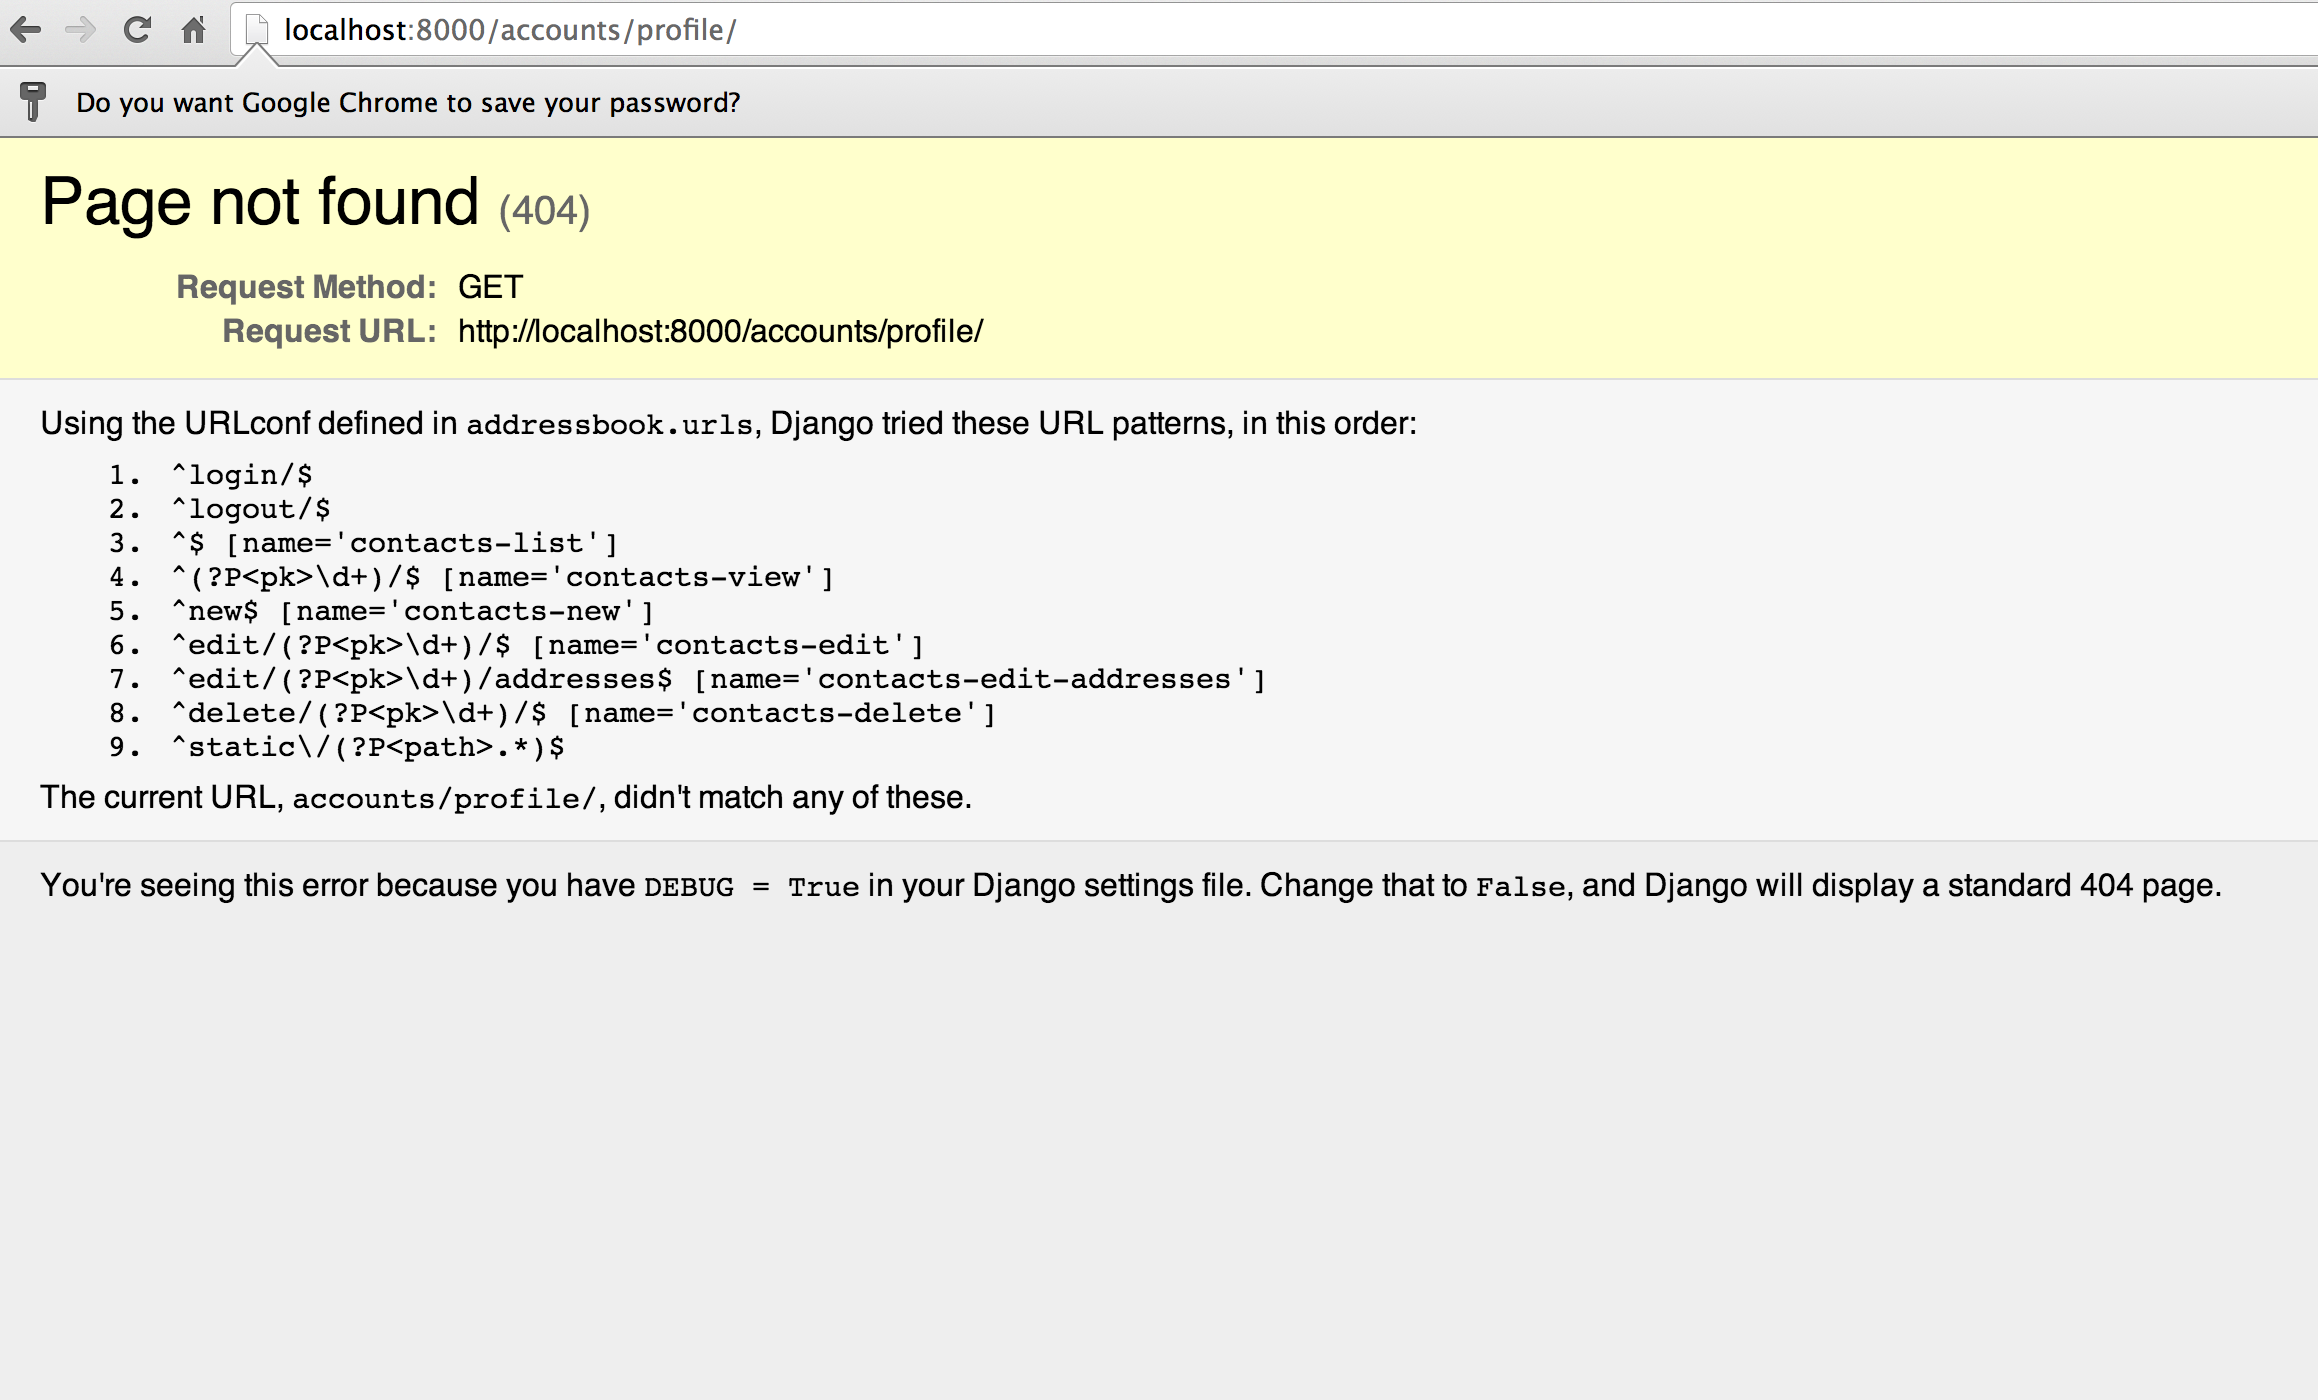
\includegraphics{authz-login-pagenotfound.png}

Wait, what? Why is it visiitng \code{/accounts/profile}? We never typed
that. The login view wants to redirect the user to a fixed URL after a
successful login, and the default is \code{/accounts/profile}. To
override that, we'll set the \code{LOGIN\_REDIRECT\_URL} value in
\code{addressbook/settings.py} so that once a user logs in they'll be
redirected to the list of contacts.

\begin{Verbatim}[commandchars=\\\{\}]
\PYG{n}{LOGIN\PYGZus{}REDIRECT\PYGZus{}URL} \PYG{o}{=} \PYG{l+s}{\PYGZsq{}}\PYG{l+s}{/}\PYG{l+s}{\PYGZsq{}}
\end{Verbatim}

Now that we can log in and log out, it'd be nice to show the logged in
user in the header and links to login/logout in the header. We'll add
that to our \code{base.html} template, since we want that to show up
everywhere.

\begin{Verbatim}[commandchars=\\\{\}]
  \PYG{n+nt}{\PYGZlt{}body}\PYG{n+nt}{\PYGZgt{}}
    \PYG{n+nt}{\PYGZlt{}div}\PYG{n+nt}{\PYGZgt{}}
      \PYGZob{}\PYGZob{} user \PYGZcb{}\PYGZcb{}
      \PYGZob{}\PYGZpc{} if user.is\PYGZus{}anonymous \PYGZpc{}\PYGZcb{}
      \PYG{n+nt}{\PYGZlt{}a} \PYG{n+na}{href=}\PYG{l+s}{\PYGZdq{}\PYGZob{}\PYGZpc{} url \PYGZsq{}django.contrib.auth.views.login\PYGZsq{} \PYGZpc{}\PYGZcb{}\PYGZdq{}}\PYG{n+nt}{\PYGZgt{}}login\PYG{n+nt}{\PYGZlt{}/a\PYGZgt{}}
      \PYGZob{}\PYGZpc{} else \PYGZpc{}\PYGZcb{}
      \PYG{n+nt}{\PYGZlt{}a} \PYG{n+na}{href=}\PYG{l+s}{\PYGZdq{}\PYGZob{}\PYGZpc{} url \PYGZsq{}django.contrib.auth.views.logout\PYGZsq{} \PYGZpc{}\PYGZcb{}\PYGZdq{}}\PYG{n+nt}{\PYGZgt{}}logout\PYG{n+nt}{\PYGZlt{}/a\PYGZgt{}}
      \PYGZob{}\PYGZpc{} endif \PYGZpc{}\PYGZcb{}
    \PYG{n+nt}{\PYGZlt{}/div\PYGZgt{}}
\end{Verbatim}


\section{Authorization}
\label{tutorial/authzn:authorization}
Having support for login and logout is nice, but we're not actually
using it right now. So we want to first make our Contact views only
available to authenticated users, and then we'll go on to associated
contacts with specific Users, so the application could be used for
multiple users.

Django includes a suite a functions and decorators that help you guard
a view based on authentication/authorization. One of the most commonly
used is \href{https://docs.djangoproject.com/en/1.5/topics/auth/default/\#django.contrib.auth.decorators.login\_required}{login\_required} (https://docs.djangoproject.com/en/1.5/topics/auth/default/\#django.contrib.auth.decorators.login\_required). Unfortunately, applying view decorators to
class based views remains \href{https://docs.djangoproject.com/en/1.5/topics/class-based-views/intro/\#decorating-class-based-views}{a little cumbersome} (https://docs.djangoproject.com/en/1.5/topics/class-based-views/intro/\#decorating-class-based-views). There are
essentially two methods: decorating the URL configuration, and
decorating the class. I'll show how to decorate the class.

Class based views have a \code{dispatch()} method that's called when an
URL pattern matches. The \code{dispatch()} method looks up the
appropriate method on the class based on the HTTP method and then
calls it. Because we want to protect the views for all HTTP methods,
we'll override and decorate that.

In \code{contacts/views.py} we'll create a class mixin that ensures the
user is logged in.

\begin{Verbatim}[commandchars=\\\{\}]
\PYG{k+kn}{from} \PYG{n+nn}{django.contrib.auth.decorators} \PYG{k+kn}{import} \PYG{n}{login\PYGZus{}required}
\PYG{k+kn}{from} \PYG{n+nn}{django.utils.decorators} \PYG{k+kn}{import} \PYG{n}{method\PYGZus{}decorator}

\PYG{k}{class} \PYG{n+nc}{LoggedInMixin}\PYG{p}{(}\PYG{n+nb}{object}\PYG{p}{)}\PYG{p}{:}

    \PYG{n+nd}{@method\PYGZus{}decorator}\PYG{p}{(}\PYG{n}{login\PYGZus{}required}\PYG{p}{)}
    \PYG{k}{def} \PYG{n+nf}{dispatch}\PYG{p}{(}\PYG{n+nb+bp}{self}\PYG{p}{,} \PYG{o}{*}\PYG{n}{args}\PYG{p}{,} \PYG{o}{*}\PYG{o}{*}\PYG{n}{kwargs}\PYG{p}{)}\PYG{p}{:}
        \PYG{k}{return} \PYG{n+nb}{super}\PYG{p}{(}\PYG{n}{LoggedInMixin}\PYG{p}{,} \PYG{n+nb+bp}{self}\PYG{p}{)}\PYG{o}{.}\PYG{n}{dispatch}\PYG{p}{(}\PYG{o}{*}\PYG{n}{args}\PYG{p}{,} \PYG{o}{*}\PYG{o}{*}\PYG{n}{kwargs}\PYG{p}{)}
\end{Verbatim}

This is a \emph{mixin} because it doesn't provide a full implementation of
a view on its own; it needs to be \emph{mixed} with another view to have an
effect.

Once we have it, we can add it to the class declarations in
\code{contacts/views.py}. Each view will have our new \code{LoggedInMixin}
added as the first superclass. For example, \code{ListContactView} will
look as follows.

\begin{Verbatim}[commandchars=\\\{\}]
\PYG{k}{class} \PYG{n+nc}{ListContactView}\PYG{p}{(}\PYG{n}{LoggedInMixin}\PYG{p}{,} \PYG{n}{ListView}\PYG{p}{)}\PYG{p}{:}

    \PYG{n}{model} \PYG{o}{=} \PYG{n}{Contact}
    \PYG{n}{template\PYGZus{}name} \PYG{o}{=} \PYG{l+s}{\PYGZsq{}}\PYG{l+s}{contact\PYGZus{}list.html}\PYG{l+s}{\PYGZsq{}}

    \PYG{k}{def} \PYG{n+nf}{get\PYGZus{}queryset}\PYG{p}{(}\PYG{n+nb+bp}{self}\PYG{p}{)}\PYG{p}{:}

        \PYG{k}{return} \PYG{n}{Contact}\PYG{o}{.}\PYG{n}{objects}\PYG{o}{.}\PYG{n}{filter}\PYG{p}{(}\PYG{n}{owner}\PYG{o}{=}\PYG{n+nb+bp}{self}\PYG{o}{.}\PYG{n}{request}\PYG{o}{.}\PYG{n}{user}\PYG{p}{)}
\end{Verbatim}

Just as \code{LOGIN\_REDIRECT\_URL} tells Django where to send people
\emph{after} they log in, there's a setting to control where to send them
when they \emph{need} to login. However, this can also be a view name, so
we don't have to bake an explicit URL into the settings.

\begin{Verbatim}[commandchars=\\\{\}]
\PYG{n}{LOGIN\PYGZus{}URL} \PYG{o}{=} \PYG{l+s}{\PYGZsq{}}\PYG{l+s}{django.contrib.auth.views.login}\PYG{l+s}{\PYGZsq{}}
\end{Verbatim}


\subsection{Checking Ownership}
\label{tutorial/authzn:checking-ownership}
Checking that you're logged in is well and good, but to make this
suitable for multiple users we need to add the concept of ownership.
There are three steps for
\begin{enumerate}
\item {} 
Record the Owner of each Contact

\item {} 
Only show Contacts the logged in user owns in the list

\item {} 
Set the Owner when creating a new one

\end{enumerate}

First, we'll go ahead and add the concept of an Owner to the Contact
model.

In \code{contacts/models.py}, we add an import and another field to our
model.

\begin{Verbatim}[commandchars=\\\{\}]
\PYG{k+kn}{from} \PYG{n+nn}{django.contrib.auth.models} \PYG{k+kn}{import} \PYG{n}{User}
\PYG{o}{.}\PYG{o}{.}\PYG{o}{.}
\PYG{k}{class} \PYG{n+nc}{Contact}\PYG{p}{(}\PYG{n}{models}\PYG{o}{.}\PYG{n}{Model}\PYG{p}{)}\PYG{p}{:}

    \PYG{n}{first\PYGZus{}name} \PYG{o}{=} \PYG{n}{models}\PYG{o}{.}\PYG{n}{CharField}\PYG{p}{(}
        \PYG{n}{max\PYGZus{}length}\PYG{o}{=}\PYG{l+m+mi}{255}\PYG{p}{,}
    \PYG{p}{)}
    \PYG{n}{last\PYGZus{}name} \PYG{o}{=} \PYG{n}{models}\PYG{o}{.}\PYG{n}{CharField}\PYG{p}{(}
        \PYG{n}{max\PYGZus{}length}\PYG{o}{=}\PYG{l+m+mi}{255}\PYG{p}{,}

    \PYG{p}{)}

    \PYG{n}{email} \PYG{o}{=} \PYG{n}{models}\PYG{o}{.}\PYG{n}{EmailField}\PYG{p}{(}\PYG{p}{)}

    \PYG{n}{owner} \PYG{o}{=} \PYG{n}{models}\PYG{o}{.}\PYG{n}{ForeignKey}\PYG{p}{(}\PYG{n}{User}\PYG{p}{)}

    \PYG{k}{def} \PYG{n+nf}{\PYGZus{}\PYGZus{}str\PYGZus{}\PYGZus{}}\PYG{p}{(}\PYG{n+nb+bp}{self}\PYG{p}{)}\PYG{p}{:}

        \PYG{k}{return} \PYG{l+s}{\PYGZsq{}}\PYG{l+s}{ }\PYG{l+s}{\PYGZsq{}}\PYG{o}{.}\PYG{n}{join}\PYG{p}{(}\PYG{p}{[}
            \PYG{n+nb+bp}{self}\PYG{o}{.}\PYG{n}{first\PYGZus{}name}\PYG{p}{,}
            \PYG{n+nb+bp}{self}\PYG{o}{.}\PYG{n}{last\PYGZus{}name}\PYG{p}{,}
        \PYG{p}{]}\PYG{p}{)}

    \PYG{k}{def} \PYG{n+nf}{get\PYGZus{}absolute\PYGZus{}url}\PYG{p}{(}\PYG{n+nb+bp}{self}\PYG{p}{)}\PYG{p}{:}

        \PYG{k}{return} \PYG{n}{reverse}\PYG{p}{(}\PYG{l+s}{\PYGZsq{}}\PYG{l+s}{contacts\PYGZhy{}view}\PYG{l+s}{\PYGZsq{}}\PYG{p}{,} \PYG{n}{kwargs}\PYG{o}{=}\PYG{p}{\PYGZob{}}\PYG{l+s}{\PYGZsq{}}\PYG{l+s}{pk}\PYG{l+s}{\PYGZsq{}}\PYG{p}{:} \PYG{n+nb+bp}{self}\PYG{o}{.}\PYG{n}{id}\PYG{p}{\PYGZcb{}}\PYG{p}{)}
\end{Verbatim}

Because Django doesn't support migrations out of the box, we'll need
to blow away the database and re-run syncdb.

XXX Perfect segue for talking about South

Now we need to limit the contact list to only the contacts the logged
in User owns. This gets us into overriding methods that the base view
classes have been handling for us.

For the list of Contacts, we'll want to override the \code{get\_queryset}
method, which returns the \href{https://docs.djangoproject.com/en/1.6/ref/class-based-views/mixins-multiple-object/\#django.views.generic.list.MultipleObjectMixin.get\_queryset}{Django QuerySet} (https://docs.djangoproject.com/en/1.6/ref/class-based-views/mixins-multiple-object/\#django.views.generic.list.MultipleObjectMixin.get\_queryset) of objects to be
displayed.

\begin{Verbatim}[commandchars=\\\{\}]
\PYG{k}{class} \PYG{n+nc}{ListContactView}\PYG{p}{(}\PYG{n}{LoggedInMixin}\PYG{p}{,} \PYG{n}{ListView}\PYG{p}{)}\PYG{p}{:}

    \PYG{n}{model} \PYG{o}{=} \PYG{n}{Contact}
    \PYG{n}{template\PYGZus{}name} \PYG{o}{=} \PYG{l+s}{\PYGZsq{}}\PYG{l+s}{contact\PYGZus{}list.html}\PYG{l+s}{\PYGZsq{}}

    \PYG{k}{def} \PYG{n+nf}{get\PYGZus{}queryset}\PYG{p}{(}\PYG{n+nb+bp}{self}\PYG{p}{)}\PYG{p}{:}

        \PYG{k}{return} \PYG{n}{Contact}\PYG{o}{.}\PYG{n}{objects}\PYG{o}{.}\PYG{n}{filter}\PYG{p}{(}\PYG{n}{owner}\PYG{o}{=}\PYG{n+nb+bp}{self}\PYG{o}{.}\PYG{n}{request}\PYG{o}{.}\PYG{n}{user}\PYG{p}{)}
\end{Verbatim}

The remaining views are responsible for showing only a single object
-- the Contact (or its addresses). For those we'll create another
mixin that enforces authorization.

\begin{Verbatim}[commandchars=\\\{\}]
\PYG{k+kn}{from} \PYG{n+nn}{django.core.exceptions} \PYG{k+kn}{import} \PYG{n}{PermissionDenied}
\PYG{o}{.}\PYG{o}{.}\PYG{o}{.}
\PYG{k}{class} \PYG{n+nc}{ContactOwnerMixin}\PYG{p}{(}\PYG{n+nb}{object}\PYG{p}{)}\PYG{p}{:}

    \PYG{k}{def} \PYG{n+nf}{get\PYGZus{}object}\PYG{p}{(}\PYG{n+nb+bp}{self}\PYG{p}{,} \PYG{n}{queryset}\PYG{o}{=}\PYG{n+nb+bp}{None}\PYG{p}{)}\PYG{p}{:}
        \PYG{l+s+sd}{\PYGZdq{}\PYGZdq{}\PYGZdq{}Returns the object the view is displaying.}

\PYG{l+s+sd}{        \PYGZdq{}\PYGZdq{}\PYGZdq{}}

        \PYG{k}{if} \PYG{n}{queryset} \PYG{o+ow}{is} \PYG{n+nb+bp}{None}\PYG{p}{:}
            \PYG{n}{queryset} \PYG{o}{=} \PYG{n+nb+bp}{self}\PYG{o}{.}\PYG{n}{get\PYGZus{}queryset}\PYG{p}{(}\PYG{p}{)}

        \PYG{n}{pk} \PYG{o}{=} \PYG{n+nb+bp}{self}\PYG{o}{.}\PYG{n}{kwargs}\PYG{o}{.}\PYG{n}{get}\PYG{p}{(}\PYG{n+nb+bp}{self}\PYG{o}{.}\PYG{n}{pk\PYGZus{}url\PYGZus{}kwarg}\PYG{p}{,} \PYG{n+nb+bp}{None}\PYG{p}{)}
        \PYG{n}{queryset} \PYG{o}{=} \PYG{n}{queryset}\PYG{o}{.}\PYG{n}{filter}\PYG{p}{(}
            \PYG{n}{pk}\PYG{o}{=}\PYG{n}{pk}\PYG{p}{,}
            \PYG{n}{owner}\PYG{o}{=}\PYG{n+nb+bp}{self}\PYG{o}{.}\PYG{n}{request}\PYG{o}{.}\PYG{n}{user}\PYG{p}{,}
        \PYG{p}{)}

        \PYG{k}{try}\PYG{p}{:}
            \PYG{n}{obj} \PYG{o}{=} \PYG{n}{queryset}\PYG{o}{.}\PYG{n}{get}\PYG{p}{(}\PYG{p}{)}
        \PYG{k}{except} \PYG{n}{ObjectDoesNotExist}\PYG{p}{:}
            \PYG{k}{raise} \PYG{n}{PermissionDenied}

        \PYG{k}{return} \PYG{n}{obj}
\end{Verbatim}

\code{ContactOwnerMixin} overrides the \code{get\_object()} method, which is
responsible for getting the object for a view to operate on. If it
can't find one with the specified primary key and owner, it raises the
\code{PermissionDenied} exception.

\begin{notice}{note}{Note:}
This implementation will return HTTP 403 (Forbidden) whenever it
cannot find the a Contact with the requested ID and owner. This
will mask legitimate 404 (Not Found) errors.
\end{notice}

We'll use the \code{ContactOwnerMixin} in all of our views. For example,
\code{ContactView} will look as follows:

\begin{Verbatim}[commandchars=\\\{\}]
\PYG{k}{class} \PYG{n+nc}{ContactView}\PYG{p}{(}\PYG{n}{LoggedInMixin}\PYG{p}{,} \PYG{n}{ContactOwnerMixin}\PYG{p}{,} \PYG{n}{DetailView}\PYG{p}{)}\PYG{p}{:}

    \PYG{n}{model} \PYG{o}{=} \PYG{n}{Contact}
    \PYG{n}{template\PYGZus{}name} \PYG{o}{=} \PYG{l+s}{\PYGZsq{}}\PYG{l+s}{contact.html}\PYG{l+s}{\PYGZsq{}}
\end{Verbatim}

Note that the order of inheritance is important: the superclasses
(\code{LoggedInMixin}, \code{ContactOwnerMixin}, \code{DetailView}) will be
checked in the order listed for methods. By placing \code{LoggedInMixin}
first, you're guaranteed that by the time execution reaches
\code{ContactOwnerMixin} and \code{DetailView}, you have a logged in,
authenticated user.


\section{Review}
\label{tutorial/authzn:review}\begin{itemize}
\item {} 
XXX

\end{itemize}

``Effective Django'' is licensed under the Creative Commons
\href{http://creativecommons.org/licenses/by-sa/4.0/}{Attribution-ShareAlike 4.0 International License} (http://creativecommons.org/licenses/by-sa/4.0/).



\renewcommand{\indexname}{Index}
\printindex
\end{document}
